\section*{Learning Objectives}
By the end of this chapter, the student should be able to:
\begin{itemize}
    \item Understand the significance of mathematical proofs and articulate their importance in Calculus and its applications.
    \item Master the technique of proof by induction and apply it to demonstrate the validity of mathematical statements.
    \item Comprehend the concept of limits and see some of their initial uses in Calculus.
\end{itemize}


\section*{Outcomes}
Upon successful completion of this chapter, students will be able to:
\begin{itemize}
    \item Apply logical rules to construct (simple) mathematical arguments.
    \item  Learn there are at least two kinds of infinity.
    \item Analyze sums of powers of integers to build a foundational understanding of integration.
    \item Calculate limits at infinity for functions that are significant in Calculus.
    \item Acquire additional knowledge about Euler's number and its unique properties.
\end{itemize}

\newpage

\section{Setting Expectations}

While this section could have been placed in the introduction to Chapter~\ref{chap:Intro}, there's a good chance that many of you would have skipped it. 

\subsection{How to Use the Textbook}

To make the most of this textbook and your learning experience, start by scanning the relevant parts of the textbook before attending (or watching) the lecture. This quick scan, which should take 15 minutes or less, will help you anticipate the main topics and identify potentially challenging points. During the lecture, focus on taking essential notes rather than copying everything verbatim—trust that the textbook has detailed explanations for most material (and besides, the instructor's live notes are posted that day). After the lecture, but before the next one, take time to rewrite and condense your notes onto one side of a single page. The act of summarizing forces you to engage with the material thoughtfully, creating a third encounter with the content after scanning and attending (watching) the lecture. By this point, you should have a solid grasp of the material. If not, this process will help you pinpoint specific questions to ask during Office Hours or study sessions. Remember, understanding comes from active engagement, not just passively reading or watching.

To further enhance your learning, review your condensed notes briefly every few days to reinforce key ideas—spaced practice improves retention. Collaborating with peers can also help you refine your understanding and tackle challenging problems together. Finally, focus on solving problems rather than memorizing formulas; calculus is best learned by doing.

If a topic in lecture went by too fast, leaving you feeling unprepared—such as understanding how to write a proof—additional help is available quickly and easily. You can use UMGPT, our version of ChatGPT, or Maizey, an AI tool indexed on the course textbook and lecture audio transcripts. To make the most of these tools, practice writing specific prompts. A broad request like ``Tell me about proofs'' may not yield useful guidance, but a focused prompt such as, ``I am struggling with writing a proof by induction and I'd like examples with clearly delineated steps and the overall thought process to help me learn,'' will provide much more relevant and actionable assistance.

When working on the homework problems, you may discover gaps in your understanding. Sometimes this happens because you zoned out during that part of the lecture—don’t worry, it happens! Other times, it’s intentional: we deliberately leave certain topics for you to learn on your own. By now, most of you have been in school for over a dozen years, so you’ve learned how to learn, right? If not, it’s never too late to take ownership of your education. Embrace these moments as opportunities to build your skills and independence—they’re as valuable as mastering the content itself.

\subsection{The Role of Lectures}

In this course, lectures are designed to be to the textbook what \textit{CliffsNotes} are to \textsc{War and Peace} or \textsc{Shakespeare}: a condensed, high-level summary that captures the key ideas while providing a framework for deeper understanding. Lectures offer a concise presentation of the most important topics, allowing you to grasp the core concepts quickly and focus on how they connect to broader ideas. 

Much like \textit{CliffsNotes}, lectures aim to be:
\begin{itemize}
    \item \textbf{Quick Summaries:} They provide a streamlined overview of complex topics, which can be especially useful for orienting yourself to the material and preparing for deeper study.
    \item \textbf{Accessible:} The straightforward structure and focused content make lectures approachable, particularly for students who may initially struggle with the density of the textbook.
    \item \textbf{Provide Supplemental Learning:} Lectures are not a replacement for reading the textbook. Instead, they complement it by helping you identify key sections and giving you the context needed to fully engage with the more detailed explanations in the book.
\end{itemize}

After attending a lecture, you are expected to read the corresponding sections of the textbook to gain a fuller understanding of the ideas introduced. The textbook provides the depth, nuance, and detailed examples necessary for mastering the material, which cannot be fully conveyed in a lecture's condensed format. 

To make the most of this approach, treat lectures as an orientation tool: focus on understanding the main points and taking essential notes. Use these notes as a guide for your textbook reading, allowing you to delve into the details with clarity and purpose. By combining the broad overview provided in lectures with the depth of the textbook, you will build a well-rounded understanding of the material and be better prepared to tackle challenging problems in homework, projects, and your engineering courses.
 

\subsection{Is this a Programming Course?}

Absolutely not! The textbook integrates programming with mathematics so that realistic problems can be solved with relative ease. Part of Calculus dread comes from the length of the algebraic manipulations that come with the application of Calculus principles, where, with each new line of calculation, comes a new opportunity for a sign error. Coding in Julia allows us to circumvent much of the drudgery and error sources. 

The coding assignments are designed to strike a balance between showcasing the power of Calculus and allowing students to complete the HW assignments within the expected 4- to 6-hour time period for a 200-level course. To achieve this, the textbook provides well-structured code templates that focus on the concepts and methods central to the problem. These templates serve as scaffolding to guide students through the logic of the computation while removing unnecessary coding overhead that could detract from the mathematical insights.

Critically, these assignments aim to marry the elegance of Calculus with the efficiency of Julia. For example, problems might involve using symbolic differentiation to derive gradients, solving systems of nonlinear equations, or numerically integrating trajectories of dynamic systems. With the provided templates, students focus on interpreting and implementing the mathematical models rather than wrestling with syntax or boilerplate code.

Some students may feel that the templates make the coding assignments too easy. However, these assignments are deliberately designed to ensure that time spent on coding enhances understanding of the mathematical principles, not debugging unrelated programming errors. The integration of written assignments alongside coding tasks ensures a well-rounded experience that highlights the theoretical underpinnings of Calculus while demonstrating its application to solving exciting and complex engineering problems.

The goal is not to transform students into programmers but to empower them with tools that extend the reach of their mathematical abilities. By reducing the cognitive load associated with low-level programming, students can engage with real-world problems that would otherwise be inaccessible within the scope of a 200-level course. Julia serves as the bridge between theoretical understanding and practical application, allowing students to see the beauty and utility of Calculus in action.

\subsection{Why Have Written Homework at All?}

The inclusion of written homework ensures that students develop the fluency needed to solve problems by hand, a skill essential for their follow-on engineering courses where manual computations will often be expected. While coding assignments demonstrate the power of computational tools like Julia, written problems serve a complementary role by emphasizing the fundamental principles of Calculus.

These written exercises provide a space for students to reflect on core concepts, strengthen their problem-solving techniques, and gain a deeper understanding of the mathematical structures that underpin their computational solutions. Together, the written and coding tasks create a balanced learning experience, showcasing the elegance and utility of Calculus while equipping students with the practical and conceptual tools necessary for their future studies.

\subsection{What if You Don't Like Julia?}

You have access to the code files on Vocareum. You can paste them into your favorite LLM and ask for them to be translated into Python, MATLAB, C++, etc., or even cleaner Julia! Coding languages come and go. Ultimately, they all provide for the manipulation of arrays, the definition of new functions, the creation of loops, and branching via if-then-else. We chose Julia over MATLAB because Julia is open-source. Moreover, it can be implemented on robots for real-time control as shown in \href{https://github.com/adubredu/KinodynamicFabrics.jl}{adubredu/KinodynamicFabrics.jl} and \href{https://arxiv.org/abs/2303.04279}{Exploring Kinodynamic Fabrics for Reactive Whole-Body Control of Underactuated Humanoid Robots}, Alphonsus Adu-Bredu, Grant Gibson, and JG.

\section{What is a Mathematical Proof? And Why are Mathematical Proofs Important?}

We ask an expert, \chatgpt :

A \textit{mathematical proof} is a logical argument that establishes the truth of a mathematical statement. It is a demonstration that, if certain fundamental statements (called axioms or premises) are assumed to be true, then another statement necessarily follows from these assumptions.

Proofs use the rules of logic combined with the axioms of the mathematical system in question to make their arguments. There are different types of proofs, such as direct proof, proof by contradiction, and proof by induction.

A \textit{direct proof} begins with the assumptions and applies the rules of logic and other mathematical truths that have already been established to arrive at the conclusion.


\textit{Proof by induction} is a method often used to prove statements about all natural numbers. It involves proving a base case (usually for the number 1 or 0) and then proving that if the statement is true for an arbitrary natural number $k>0$, it's also true for the number $k+1$.

\textit{Proof by contradiction} (also known as reductio ad absurdum) assumes that the statement to be proved is actually false, and then shows that this assumption leads to an absurdity. This then means that the statement cannot be false, and hence must actually be true because we are using ``binary logic'' (any statement is either \textbf{T} or \textbf{F}; there is nothing in between).


Mathematical proofs are crucial for a number of reasons:
\begin{enumerate}
\renewcommand{\labelenumi}{(\alph{enumi})}
\setlength{\itemsep}{.2cm}
    \item \textit{Certainty:} Unlike in many other fields, in mathematics, knowledge can be established beyond a shadow of a doubt. A proof guarantees that, given the acceptance of the axioms, the conclusion must be true.
    \item \textit{Building Blocks:} Each proven statement becomes a tool that mathematicians can use in further proofs. Mathematics is built up from layers upon layers of proven statements.
    \item \textit{Understanding:} The process of creating a proof often leads to a deeper understanding of the mathematical structure being studied.
    \item \textit{Discovery:} Sometimes, the process of proving a statement can lead to the discovery of new mathematical facts or even whole areas of mathematics.
    \item \textit{Rigor:} Proofs provide a standard of rigor that helps prevent errors in mathematical reasoning. This rigor is crucial in areas such as computer programming and algorithm design, where a small error in reasoning can lead to significant problems. 
\end{enumerate}

\begin{tcolorbox}[title = {Mathematical Proofs Promote Understanding}, sharp corners, colback=lightgold, colframe=black, coltitle=white, breakable, fonttitle=\bfseries]
In short, mathematical proofs are the cornerstone of mathematical knowledge, providing certainty, depth of understanding, and a rigorous basis for further discovery. We'll add one more reason they are important: some things that seem ``obviously false'', even to the larger Mathematical Community, can turn out to be true, and vice versa! In the next Section, we'll use a famous example to accomplish two things: (1) learn about countable and uncountable sets and (2) underline that you can be right even when everyone tells you that you are wrong. A sad example of the latter is  \href{https://en.wikipedia.org/wiki/Georg_Cantor}{Georg Cantor}, whose surprising discovery about the nature of infinity led to public opposition and personal attacks. Mathematics being as controversial as \href{https://en.wikipedia.org/wiki/Scopes_trial}{evolution}? You cannot make this stuff up! Please read on.
\end{tcolorbox}

\textbf{Related Videos:}
\begin{itemize}
    \item \href{https://www.youtube.com/shorts/VFbyGEZLMZw?feature=share}{Don't let it fool you} by \threebb ~(moral of the story: patterns often break).
    \item \href{https://youtu.be/TvQt372BLT8}{Proofs Are Awesome! Here's Why!} 
Math Time With Professor Prime (a short low-key pep talk).
\item \href{https://youtu.be/X_xR5Kes4Rs}{Is math discovered or invented?} a TED-ED talk by Jeff Dekofsky (asks the question, ``does math exist independent of humans'').
\end{itemize}



\section{Vocabulary and Helpful Notation} 
The following definitions borrow liberally from \href{https://users.math.msu.edu/users/duncan42/AxiomNotes.pdf}{Math 299}, Michigan State University. In this course, you will rarely be asked to write proofs yourself. You will be asked to read them from time to time. In lectures and \textbf{quizzes}, we will use the terminology, vocabulary, and shorthand notation called out below.


\textbf{Terminology:}
\begin{itemize}
\item \textit{Definition:} A precise explanation of the mathematical meaning of a term or concept.
\item \textit{Axiom:} A fundamental principle or assumption that is accepted as true without proof in a mathematical system.
\item \textit{Theorem:} A mathematical statement that has been proven to be true.
\item \textit{Lemma:} A mathematical statement that is proven true and used as a stepping stone in the proof of other statements.
\item \textit{Claim:} A mathematical statement that is made as a step towards proving a theorem or to highlight an important property of a mathematical object. When used as a stepping stone to prove something else, Claims are essentially equivalent to Lemmas. When a Claim is used to highlight an important property, it is a ``baby'' Proposition.  
\item \textit{Proposition:} A mathematical statement that is less central but nonetheless true and interesting.
\item \textit{Corollary:} A mathematical statement that is a straightforward deduction from a theorem or proposition.
\item \textit{Proof:} The logical reasoning that demonstrates why a statement is true.
\item \textit{Conjecture:} A mathematical statement that is believed to be true, but for which no proof has been established. Or, a communication of a potentially true statement that the author hopes to prove or that the mathematical community seeks to prove. \href{https://en.wikipedia.org/wiki/Fermat%27s_Last_Theorem}{Fermat's Last Theorem} was a Conjecture until it was proven by \href{https://en.wikipedia.org/wiki/Wiles%27s_proof_of_Fermat%27s_Last_Theorem}{Wiles} in 1995.
\end{itemize}

We will mostly use just definitions and propositions so that we do not get tied up in the hierarchy of theorems, lemmas, etc. We will not take this to extremes, by calling the very well-known ``Pythagorean Theorem'' the ``Pythagorean Proposition'', or awkwardly referring to the ``Binomial Proposition''.

\bigskip

\emstat{
\textbf{Crib Notes for Proofs:} where $P$ and $Q$ are logical statements. They can be either true (denoted \textbf{T}) or false (denoted \textbf{F}). Because we use binary logic, there is no in-between value, such as ``maybe''. Statement are either  \textbf{T} or \textbf{F}.\\

In the following, you might have in mind, $P:~\det(A) \neq 0$ and $Q: A$ is a square invertible matrix, or, $P: \text{ the rows of } A$ are linearly independent and $Q: Ax = b$ has a minimum norm solution.
\begin{itemize}
        \item  $\neg$ or $\sim$  denotes the logical operation ``NOT'', where $\neg \textbf{T}=\textbf{F}$ and $\neg \textbf{F}=\textbf{T}$. Both symbols will be used interchangeably in these notes. 
        \item  $P \implies Q$ represents ``if statement $P$ is true, then statement $Q$ is also true''.
        \item  $P \iff Q$ indicates that ``$P$ is true if and only if $Q$ is true". Although $P \textrm{ iff } Q$ is a valid expression, it will be seldom used in these notes.
        \item  $P \iff Q$ is logically equivalent to:
        \begin{itemize}
            \item[]  (a) $P \implies Q$ and
            \item[]  (b) $Q \implies P$.
        \end{itemize}
        \item  The \emph{contrapositive} of $P \implies Q$ is denoted as $\neg Q \implies \neg P$.
        \item  The \emph{converse} of $P \implies Q$ is expressed as $Q \implies P$. It is crucial to note that $P \implies Q$ does not generally imply $Q\implies P$ and vice versa. If they were equivalent, there would be no need for $P \iff Q$.
        \item  The relation $(P \implies Q) \Longleftrightarrow (\neg Q \implies \neg P)$ indicates that these two statements are logically equivalent. Although they are equivalent, one may be easier to use in a proof than the other.
        \item  \emph{Logical AND}: $P_1 \land P_2$ is read as ``$P_1$ AND $P_2$''. It holds true when both $P_1$ and $P_2$ are true.
        \item  \emph{Logical OR}: $P_1 \lor P_2$ is interpreted as ``$P_1$ OR $P_2$". It is true when at least one of $P_1$ or $P_2$ is true. In this course, we use the ``inclusive OR'', which means $\textbf{T} \lor \textbf{T} = \textbf{T} \lor \textbf{F} = \textbf{F} \lor \textbf{T} = \textbf{T}$, where \textbf{T} stands for true and \textbf{F} stands for false.
        \item  Q.E.D. is an abbreviation of the Latin phrase ``quod erat demonstrandum'', which translates to ``what was to be demonstrated''. It is used to indicate the completion of a proof. Nowadays, you more frequently see $\square$ or $\blacksquare$ instead of Q.E.D. 
\end{itemize}
}
 
    
    \textbf{Warning:} In the beginning, it is quite frequent that students confuse the meanings of \emph{contrapositive} and \emph{converse}. Just be careful. With practice, it becomes second nature. The fact that they both start with ``con-'' is not helpful!

\bigskip


 
\begin{tcolorbox}[colback = mylightblue, title=\textbf{(Optional Read:) Symbology of Mathematics:}, breakable]


\begin{definition} Mathematical Shorthand:
   
\begin{enumerate}
\renewcommand{\labelenumi}{(\alph{enumi})}
\setlength{\itemsep}{.2cm}
                      
        \item  $\forall$ means ``\textbf{for every}'', `\textbf{`for all}'', or ``\textbf{for each}'' as in $\forall~x\in \real$, $x^0:= 1$, which means that for all real numbers $x$, we define $x^0$ to stand for the number one. Continuing in this vein, the notation $\forall~k \in \nat$ and $\forall~x\in \real$, $x^k:= x\cdot x^{k-1}$, which means that for all counting numbers, and for all real numbers $x$, we define $x^k$ to stand for the product of $x$ times $x^{k-1}$. We note that $x^1$ makes sense because $x^1:= x \cdot x^0 = x \cdot 1$, and we know how to form the product $x \cdot 1$ within the set of real numbers.

        \item  $\exists$ means ``\textbf{there exist(s)}'', ``\textbf{there is/are}'', ``\textbf{for some}", ``\textbf{for at least one}'' as in $\exists ~x\in [0, \pi/2]$ such that $\sin(x) = \frac{\sqrt{2}}{2}$, which reads, there exits at least one point $x$ in the interval from zero to $\pi/2$ such that $\sin(x) = \frac{\sqrt{2}}{2}$. Or let $A$ and $B$ be sets. Then $f:A \to B$ is a function if, $\forall ~a \in A, \exists~b \in B$, such that $f(a) = b$, that is, $f$ is a function from $A$ to $B$ if for all elements $a$ in the set $A$ there is some element $b$ in the set $ B$ such that $f(a) = b$. Or a final example, $\forall~x \in \real$ and $\forall~\epsilon > 0$, $\exists~ r \in \rat$ such that $|x-r| < \epsilon$, which means: for every real number $x$ and every positive number $\epsilon$ no matter how small, there exists a rational number $r$ that approximates $x$ with an error that is less than or equal to $\epsilon$ (or you could say, approximates $x$ within a tolerance of $\epsilon$). When we do numerical computations on a computer, we use rational approximations of real numbers. In that case, the smallest positive number that, when added to 1, yields a result different from 1 in the machine's arithmetic is called \textit{machine epsilon}. For single-precision IEEE 754 standard floating-point format (often used in the float data type in programming languages), the machine epsilon is $ 2^{-23}$, or approximately $1.19 \times 10^{-7}$, and for double-precision IEEE 754 standard floating-point format (often used in the double data type in programming languages), the machine epsilon is $ 2^{-52}$, or approximately $2.22 \times 10^{-16}$.

        \item $\nexists$ means ``\textbf{there do/does not exist}'', ``\textbf{there is no element}'', or ``\textbf{there are no elements}'', as in $\nexists ~x\in \real$ such that $x \cdot 0 = 1$, which is how you would write that the number zero does not have a multiplicative inverse.  Or another example, $\tan(x)$ is not a function from $\real$ to $\real$ because $\pi/2$ is in the domain $\real$, but $\nexists y \in \real$ (used here as the codomain) such that $\tan(\pi/2) = y$. Recall that a function $f:A \to B$ \textbf{must assign} to each element of the domain, $A$, an element in the codomain, $B$. 
    
\end{enumerate}
\end{definition}

Initially, these symbols might appear as unnecessary complexities. \textcolor{red}{\bf Yet, they aim to serve as a concise language}, enabling precise and efficient communication of concepts that we encounter regularly. With practice, you will come to appreciate them just as much as you appreciate Descartes' notation for unknowns. 

\end{tcolorbox}

\section{Proofs by Induction, Some Finite Sums, and Their Applications}

The only way to learn proofs is by doing them. 


\subsection{Two Finite Sums via Induction}

\begin{logicColor}{First Principle of Induction (Standard Induction)}{PrincipleInduction}
      Let $P(n)$ denote a statement about the counting numbers with the following properties:
        \begin{itemize}
            \item[] (a) \textbf{Base case:} $P(1)$ is true
            \item[] (b) \textbf{Induction hypothesis:} For all $k\ge 1$, if $P(k)$ is true, then $P(k+1)$ is true.
        \end{itemize}
Then $P(n)$ is true for all $n \geq 1$.
    
\end{logicColor}

\begin{rem}
Suppose the base case involves an integer $k_0 \neq 1$. Then you can re-index things and reduce it to the base case having $k_0=1$. Alternatively, you assume that $P(k)$ true for $k \ge k_0$ implies  $P(k+1)$ is true, and then you get $P(n)$ is true for all $n \geq k_0$. A common mistake is not to use the correct base case. For example, you can read about ``how to prove by induction'' that all  \href{https://en.wikipedia.org/wiki/All_horses_are_the_same_color}{horses are the same color}. 
\end{rem} 

    \bigskip
\begin{example} 
\label{ex:SumFirstIntegersPower1}
Let's prove the \textbf{Claim:}  For all $n \geq 1$, 
\begin{equation}
\label{eqn:SumFirstIntegers}
    1+2 + 3 + \cdots + n = \frac{n(n+1)}{2}.
\end{equation}
\end{example}

\textbf{Proof:} 

   \begin{itemize}
    \item  \textbf{Step 0:} Write down $P(n)$: $1+2 + 3 + \cdots + n = n(n+1)/2$, the statement that is to be proved. 
        \item \textbf{Step 1:} Check the base case, $P(1)$: For  $n=1$, we have that  is $ 1 = 1$ for the left side (the sum of the first one integer), and for the right side, $ n(n+1)/2 = 1\cdot (1+1)/2 = 2/2 = 1 $. Because $1=1$, the base case is true. 
        \item \textbf{Step 2:} Show the induction hypothesis is true. That is, assuming that $P(k)$ is true, show that $P(k+1)$ is true. For us,  
 $$P(k+1): (1+2+\dots +k)+(k+1) = (k+1)\cdot(k+2)/2.$$
 Often, showing that $P(k) = \textbf{T} \implies P(k+1) = \textbf{T}$ involves re-writing the terms in $P(k+1)$ as a sum of terms that show up in $P(k)$, plus another term.\\
  
    \end{itemize}
 
 
For the induction step, we assume that
$$
        P(k): 1+2 + 3 + \cdots + k = k\cdot(k+1)/2
$$
is true. Next, we note there are terms in $P(k+1)$ that are common to $P(k)$, namely 
$$ 
(1+2+\dotsb+k ) + (k+1) = \underbrace{(1+2+\dotsb+k)}_{k\cdot (k+1)/2} +(k+1) = k\cdot (k+1)/2 + (k+1),
$$
because we assumed that $P(k)$ holds. 
Then, by the accepted rules of arithmetic, 
$$       
k(k+1)/2 + (k+1) =(k+1)\cdot ( k/2 + 1 ) =(k+1)\cdot (k+2)/2,
$$
and we deduce that 
$$  (1+2+\dots +k)+(k+1) = (k+1)\cdot(k+2)/2,$$
and therefore, $P(k+1)$ is true. Because we have shown that $P(1)$ is true and for all $k\ge 1$, $P(k) \implies P(k+1)$, by the Principle of Induction, we conclude that for all $n\ge 1$,
$$1+2 + 3 + \cdots + n = n(n+1)/2,$$
that is, \eqref{eqn:SumFirstIntegers} holds.
\Qed
\bigskip


\begin{rem}
If you run into a case where base case $P(1)$ seems so totally trivial that you are unsure whether there is anything to show, it's OK to check $P(2)$, just to convince yourself that it is true too. In our case, you would have checked $P(2): 1 + 2 = 2 \cdot3/2 $; since this is easily established to be true, you may now be more confident of your proof. If you do one more, $P(3): 1 + 2 + 3 = 3\cdot 4/2$, you are now on a roll and ready to attack the general case by induction. Bottom line: Initially, it's natural to be tentative when you write a proof. \textcolor{red}{\bf It takes practice to learn the art of proving things.} \textbf{In this course, writing proofs is not a core skill we are trying to develop.} \textcolor{blue}{\bf Instead, we want you to respect that proofs are important because they explain why something is true}. They turn a mathematical result from  ``black box'' (opaque, unclear, huh?, pure manipulation of symbols) to ``white box'' (clear, transparent, understandable, Oh, that's why!, feeling like you know what you are doing)\footnote{The terms ``black box'' and ``white box'' are commonly used in various fields, including systems engineering, computing, and business, with their exact meaning depending on the context. 

\begin{itemize} 

\item \textbf{Black Box Testing/Modeling:} In black box testing or modeling, the internal workings of the system or model are not known or considered. It's called a ``black box'' because the system is opaque; we can't see what's happening inside. Instead, we focus on the input and output. We provide certain inputs, and then test to see if the output is as expected. In the context of AI, a black box model is a system where we can observe the input and output, but not the internal decision-making process. For example, deep learning models are often considered black boxes because, although they can make highly accurate predictions, it's difficult to understand how they arrived at a particular decision.

\item \textbf{White Box Testing/Modeling:} In white box testing or modeling, we do have access to the internal workings of the system or model. This type of testing is sometimes called ``clear box" or ``glass box" testing. We not only examine input and output but also the processes that lead from one to the other. For example, a decision tree can be considered a white box model because it's possible to follow the path from beginning to end to understand exactly how a decision is made.
\end{itemize}
In a similar sense, a mathematical proof provides the steps that show us how to go from the hypotheses (i.e., input) to the claimed result (i.e., output). Without proofs, we are taking results on faith.
}. 
\end{rem} 


\begin{example} 
\label{ex:SumIntegersSquared}
Let's prove the \textbf{Claim:}  For all $n \geq 1$, 
\begin{equation}
    \label{eqn:SumFirstIntegersSquared}
    1^2+2^2 +  \cdots + n^2 = \frac{n(n + 1)(2n + 1)}{6}
\end{equation}
\end{example}

\textbf{Proof:} 


Proofs can be written in many different ways. Let's approach this proof a bit differently by defining 
\begin{equation}
    \begin{aligned}
    L(n)&:= 1^2+2^2  + \cdots + n^2, \text{ the left side of the Claim}, \\
    R(n) &: =n(n+ 1)(2n + 1)/6, \text{the right side of the Claim.}
    \end{aligned}    
\end{equation} 
We want to show for all counting numbers $n\ge 1$,
$$ P(n) \text{ is true, that is, } L(n)=R(n).$$


    \begin{itemize}
    \item \textbf{Step 0:} Write down $P(k)$: $L(k)=R(k)$. 
        \item \textbf{Step 1:} Check the base case, $P(1)$: For  $k=1$, we have that $L(1) = 1$ and $R(1) =  1 \cdot (1 + 1) \cdot (2 + 1)/6 = 1$ and hence the base case is true. 
         \item \textbf{Step 2:} Let's check one more just so we get the hang of it, $P(2)$: we have that $ L(2)= 1^2 + 2^2= 5$ and $R(2)= 2 \cdot (2 + 1)(2\cdot 2 + 1)/6 =2 \cdot  (15)/6 = 5$, and hence $L(2)=R(2)$, showing that $P(2)$ holds. Our confidence is higher! 
        \item \textbf{Step 3:} Show the induction hypothesis is true. That is, using the fact that $P(k)$ is true for some $k \ge 1$, show that $P(k+1)$ is true.\\
  
    \end{itemize}

When we assume that $P(k)$ is true, we are assuming that
$$
        L(k) = R(k). 
$$
To see if this implies $L(k+1) = R(k+1)$, we first evaluate  
 $$L(k+1)= \underbrace{1 ^2 +2^2 \cdots +k^2}_{L(k)} + (k+1)^2 = L(k) + (k+1)^2.$$
Using the induction hypothesis, namely, $L(k)=R(k)=k(k+1)(2 k + 1)/6$, we compute 
\begin{equation}
    \label{eq:SumIntegersSqauredLeft}
    \begin{aligned}
        L(k+1)&= L(k) + (k+1)^2 \\
        &= \underbrace{k(k+1)(2 k + 1)/6}_{L(k)} +  (k+1)^2  \\
        &= \underbrace{(2k^3+3k^2+k)/6}_{k(k+1)(2 k + 1)/6} +  \underbrace{(k^2+2k+1)}_{(k+1)^2} \\
        &= (k^3/3 + k^2/2 + k/6)+ (k^2+2k+1) \\
        \\
        &= k^3/3 + 3  k^2/2 + 13 k/6  + 1.
    \end{aligned}
\end{equation}
There was some ``messy'' algebra, but nothing too taxing.\\

Next, we plug $(k+1)$ into the definition of $R(k)$ to evaluate
\begin{equation}
    \label{eq:SumIntegersSqauredRight}
    \begin{aligned}
        R(k+1)&= (k+1)\cdot((k+1) + 1) \cdot (2(k+1) +1)/6  \\
        & = (k+1)\cdot(k+2) \cdot (2k+3)/6  \\
        &= (k+1) \cdot (2k^2 + 7k + 6)/6 \\
        &=  k^3/3 + 3k^2/2 + 13k/6 + 1.
    \end{aligned}
\end{equation}
Once again, there was some ``messy'' algebra, but nothing too taxing.\\

Comparing \eqref{eq:SumIntegersSqauredLeft} and \eqref{eq:SumIntegersSqauredRight}, we see that indeed, $L(k+1) = R(k+1)$, and therefore $P(k+1)$ is true. Because we have shown that $P(1)$ is true, and for all $k\ge 1$, $P(k) \implies P(k+1)$, by the Principle of Induction, we conclude that for all $n\ge 1$,
$$ 1^2+2^2 +  \cdots + n^2 = n(n + 1)(2n + 1) / 6.$$
\Qed
\bigskip

This example, from \href{https://youtu.be/kLET3c9qRgo}{Prove that $n^3 +11n$ is divisible by 6} by PrimeNewtons, is included to show a different style of proof by induction, always with the goal of enhancing your understanding. A counting number (positive integer) $i \in \nat$ is divisible by 6 if there exists another integer $m \in \nat$ such that $i = 6 \cdot m$; in other words, $\frac{i}{6}$ is also a counting number.

\begin{exercise} 
Use induction to show that for all $n\in \nat$,  $n^3 +11n$ is divisible by 6.
    
\end{exercise}

\solution We want to show for all counting numbers $n\ge 1$,
 $P(n): n^3 + 11n = 6 \cdot m$, for some counting number $m$. \\

 \textbf{Base Case: $\bm{n=1}$:} $1^3 + 11\cdot 1 = 12 = 2 \cdot 6$, and hence the base case is true.\\

 \textbf{Induction Step:} We show that if $P(k)$ is true for some $k\ge 1$, then $P(k+1)$ is true. \\

 We first use basic algebra to arrive at 
 \begin{equation}
 \label{eq:ncubedplus11n}
     \begin{aligned}
         (k+1)^3 + 11 \cdot (k+1) & = \left(  k^3 + 3 k^2 + 3 k + 1\right) + \left( 11 k + 11 \right) \\
         & = \left( k^3 + 11 k\right) + 3 \cdot \left( k^2 + k + 4\right) .
     \end{aligned}
 \end{equation}
 Because $P(k)$ holds, there exists $m_1 \in \nat$ such that 
 $ \left( k^3 + 11 k\right) = 6 m_1$. We prove below that $\left( k^2 + k + 4\right)$ is even for all counting numbers $k$, and hence there exists $m_2$ such that $\left( k^2 + k + 4\right) = 2 m_2$. Substituting these facts into \eqref{eq:ncubedplus11n} gives
\begin{align*}
         (k+1)^3 + 11 \cdot (k+1) &  = \left( k^3 + 11 k\right) + 3 \cdot \left( k^2 + k + 4\right) \\
         & = 6 m_1 + 3 \cdot 2 m_2 \\
         & = 6 \cdot \left( m_1 + m_2\right).
 \end{align*}
 This completes the proof because, $m_1 + m_2$, the sum of two counting numbers, is another counting number.\\

 \textbf{Claim:} $k^2 + k + 4$ is even for all counting numbers $k$.

 \textbf{Proof:}  Uses basic properties of counting numbers, whose proofs you can either provide or seek online. If $k$ is odd, then so is $k^2$. Because the sum of two odd numbers is even, we have that $k^2+k$ is even. Finally, adding the even number $4$ to the even number $k^2+k$ gives an even number.  Next, if $k$ is even, so is $k^2$. Because the sum of two even numbers is even, we have that $k^2+k$ is even. Finally, adding the even number $4$ to the even number $k^2+k$ gives an even number.\\

 \textbf{Note:} The information we learned from $P(k)$, namely that $k^3 + 11 k$ is divisible by $6$, needed to be augmented with an additional fact about counting numbers, namely that $ k^2 + k + 4$ is always even.

 \Qed
 
 \bigskip

   
    \begin{figure}[htb]%
\centering
\subfloat[]{%
    %
	\centering
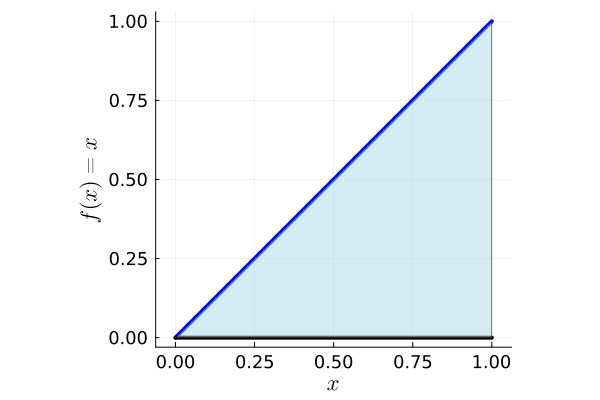
\includegraphics[width=0.45\columnwidth]{graphics/Chap02/AreaTriangleExact.png}}%
\hspace{5pt}%
\subfloat[]{%
    %\label{fig:MonotonicB}%
	\centering
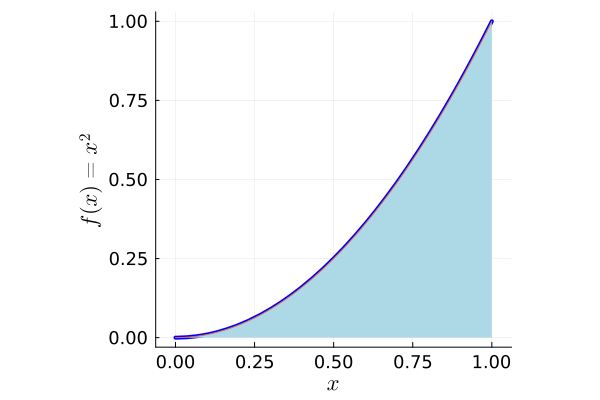
\includegraphics[width=0.45\columnwidth]{graphics/Chap02/AreaParabolaExact.png}}%
    \caption[]{Areas under curves. In blue, the areas under two curves between $x=0$ and $x=1$ are shown. (a) For a triangle, we know the formula for its area, $\frac{1}{2}b \cdot h$, one-half base times height! (b) For the parabola $y=x^2$, we do not have a simple formula for its area. We'll develop a method to estimate lower and upper bounds for the computation of areas. We'll first show how our estimate works for the triangle, and then apply it to the parabola. Sounds like a plan?}
    \label{fig:InitialAreasTriangleParapbola}
\end{figure}

\bigskip
\textbf{Related Videos:}
\begin{itemize}
    \item Basic: \href{https://www.youtube.com/watch?v=wblW_M_HVQ8}{Proof by induction | Sequences, series and induction | Precalculus} by Khan Academy.
    \item Basic: \href{https://www.youtube.com/watch?v=tHNVX3e9zd0}{Mathematical Induction Practice Problems} by the Organic Chemistry Tutor.
    \item More Advanced: \href{https://www.youtube.com/watch?v=w362XRZy5as}{Prove by induction, Sum of the first n cubes, $1^3+2^3+3^3+...+n^3$} by \bprp.
    \item Quite Advanced: \href{https://www.youtube.com/watch?v=OI-nSvpZTpE}{Introduction to Proof by Induction [Discrete Math Class]} by Mathematical Visual Proofs.
\end{itemize}




\subsection{The Amazing Power of the Rectangle: Finding Area under a Curve}
\label{sec:ApproximatingAreaFiniteSumRectangles}

In this section, we will use what we have learned so far to lay the foundations for computing areas under the simple ``curves'' shown in Fig.~\ref{fig:InitialAreasTriangleParapbola}, namely a line and a parabola, \textbf{assuming only knowledge of the area of a rectangle!} How can we do this? . We will follow Archimedes' basic plan: create both a lower bound and an upper bound for our desired quantity (for Archimedes, it was the circumference of the circle, here, it is area under the curve), and then show that we can make the lower and upper bounds approach one another. You may wish to refer to Fig.~\ref{fig:ArchimedesAndPi} and the text around it to refresh your memory. 

The curves in Fig.~\ref{fig:InitialAreasTriangleParapbola} are monotonically increasing, making it particularly easy to formulate upper and lower bounds for their areas by summing the areas of carefully chosen rectangles. We already know a formula for the area of a triangle, namely, one-half base times height, $\frac{1}{2}b \cdot h$, giving us 0.5 for the area in Fig.~\ref{fig:InitialAreasTriangleParapbola}-(a). What is the area for the parabola in Fig.~\ref{fig:InitialAreasTriangleParapbola}-(b)?

    \begin{figure}[htb]%
\centering
\subfloat[]{%
    %
	\centering
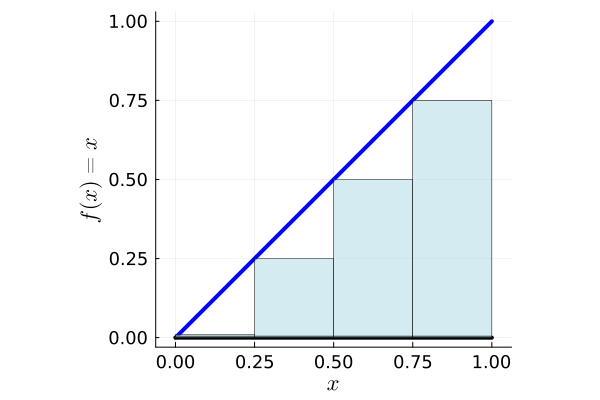
\includegraphics[width=0.45\columnwidth]{graphics/Chap02/AreaTriangleUnderApprox.png}}%
\hspace{5pt}%
\subfloat[]{%
    %\label{fig:MonotonicB}%
	\centering
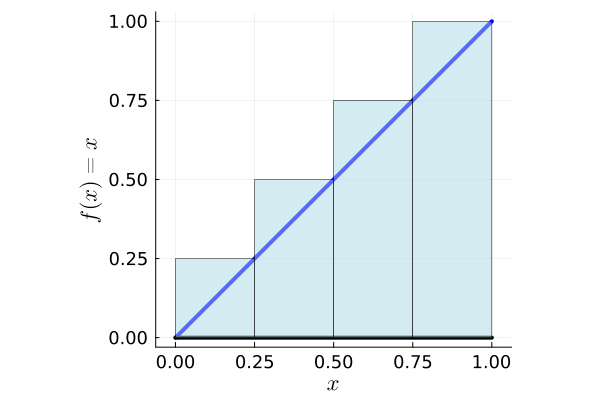
\includegraphics[width=0.45\columnwidth]{graphics/Chap02/AreaTriangleOverApprox.png}}%
\hspace{5pt}%
\subfloat[]{%
    %\label{fig:MonotonicB}%
	\centering
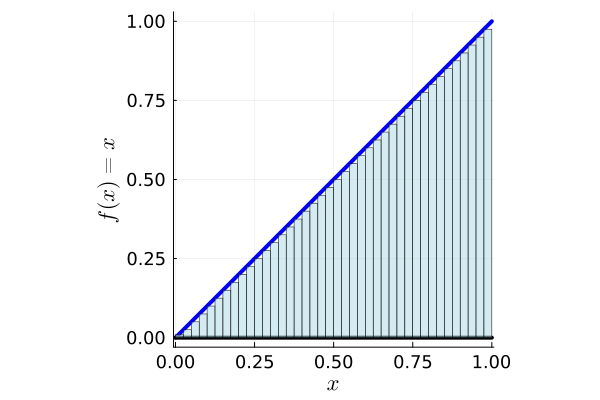
\includegraphics[width=0.45\columnwidth]{graphics/Chap02/AreaTriangleUnderApprox40.png}}%
\hspace{5pt}%
\subfloat[]{%
    %\label{fig:MonotonicB}%
	\centering
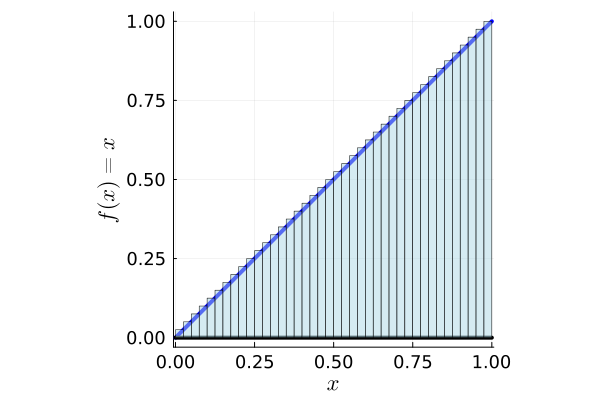
\includegraphics[width=0.45\columnwidth]{graphics/Chap02/AreaTriangleOverApprox40.png}}%
    \caption[]{Under- and overapproximations for the area of a triangle defined by a line of slope one through the origin. (a) An underapproximation for the triangle defined by $f(x)=x,~ 0 \le x \le 1$. (b) An overapproximation for the triangle defined by $f(x)=0,~ 0 \le x \le 1$. For (a) and (b), $n=4$ and thus $\Delta x = 0.25$, while for (c) and (d), $n=40$ and $\Delta x = 0.025$.}
    \label{fig:ApproxAreaTriangle}
\end{figure}

\begin{methodColor}{Lower and Upper Bounds for Area Under an Increasing Function}{FirstTakeAreaLowerUpperBounds}

\textbf{Approximating Area:} We seek to estimate the area under an increasing function $f:[a, b] \to \real$, where $a < b$. We first divide the interval $[a, b]$ into $n >1$ evenly spaced subintervals, $[x_i, x_{i+1}]$, where
\begin{equation}
    \begin{aligned}
        \Delta x :=& \frac{b-a}{n} \\
           x_i :=& a + (i-1) \cdot \Delta x,
    \end{aligned}
\end{equation}
so that 
    \begin{gather}
        a = x_1 < x_2 < \cdots < x_{n} < x_{n+1} = b\\
        x_{i+1} = x_i + \Delta x, ~1 \le i \le n \\
          f(x_1) \le f(x_2)  \le \cdots \le f(x_{n}) \le  f(x_{n+1}). 
    \end{gather}
    \begin{itemize}
        \item We underestimate the area between $[x_i, x_{i+1}]$ by a rectangle of height $h_i^{\rm Low}:=f(x_i)$ and base $b_i:= \Delta x$. This is an \textbf{underapproximation} because $h_i^{\rm Low}:=f(x_i) \le f(x)$ for all $x \in [x_i, x_{i+1}]$. We underestimate the  total area between $[a, b]$ by summing up the underapproximations,
        \begin{equation}
            {\rm Area}^{\rm Low}_n : = \sum_{i=1}^n h_i^{\rm Low} \cdot b_i =  \sum_{i=1}^n f(x_i)\cdot \Delta x.
        \end{equation}
        \item We overestimate the area between $[x_i, x_{i+1}]$ by a rectangle of height $h_i^{\rm Up}:=f(x_{i+1})$ and base $b_i:= \Delta x$. This is an \textbf{overapproximation} because $ h_i^{\rm Up}:=f(x_{i+1}) \ge f(x)$ for all $x \in [x_i, x_{i+1}]$.  We overestimate the  total area between $[a, b]$ by summing up the overapproximations,
        \begin{equation}
            {\rm Area}^{\rm Up}_n : = \sum_{i=1}^n h_i^{\rm Up} \cdot b_i =  \sum_{i=1}^n f(x_{i+1})\cdot \Delta x.
        \end{equation}
        \item See Fig.~\ref{fig:ApproxAreaTriangle} and Fig.~\ref{fig:ApproxAreaParabola}.
    \end{itemize} 

  Then, just like with Archimedes, we have that for all $n > 1$, 
    $${\rm Area}^{\rm Low}_n \le {\rm Area} \le  {\rm Area}^{\rm Up}_n,   $$
    where ${\rm Area}$ is the true area under the curve between the values $x=a$ and $x=b$. Moreover, as we take $n$ larger and larger, the lower and upper bounds will approach one another, giving us the ability to approximate the area with arbitrary accuracy.
\end{methodColor}

Let's carry out this method for $f(x)=x$, $a=0$ and $b=1$. Then with $n>0$, we have $\Delta x =\frac{1}{n}$, $x_i = (i-1) \Delta x$, $f(x_i)= (i-1) \Delta x$, and 
\begin{equation}
\begin{aligned}
    {\rm Area}^{\rm Low}_n :&=   \sum_{i=1}^n f(x_i)\cdot \Delta x \\
    &=   \sum_{i=1}^n \left((i-1) \Delta x\right) \cdot \Delta x  \\
    &=  \sum_{i=1}^n\left((i-1) \frac{1}{n}\right) \cdot \frac{1}{n} \\
    &= \frac{1}{n^2} \cdot  \sum_{i=1}^n (i-1) ~~~~(\text{because } n \text{ is a constant, we take it out of the sum}) \\
     &= \frac{1}{n^2} \cdot  \sum_{i=1}^{n-1} i ~~~~(\text{change of index}) \\
    &= \frac{1}{n^2} \cdot \frac{(n-1) (n)}{2} ~~~~(\text{by Example }\ref{ex:SumFirstIntegersPower1})\\
    &= \frac{1}{2} - \frac{1}{2n},
\end{aligned}
\end{equation}
Similarly, 
\begin{equation}
\begin{aligned}
    {\rm Area}^{\rm Up}_n :&=   \sum_{i=1}^{n} f(x_{i+1})\cdot \Delta x \\
    &=   \sum_{i=1}^n \left(i \Delta x\right) \cdot \Delta x  \\
    &=  \sum_{i=1}^n\left(i \frac{1}{n}\right) \cdot \frac{1}{n} \\
    &= \frac{1}{n^2} \cdot  \sum_{i=1}^n i ~~~~(\text{because } n \text{ is a constant, we take it out of the sum}) \\
    &= \frac{1}{n^2} \cdot \frac{n(n+1)}{2}  ~~~~(\text{by Example }\ref{ex:SumFirstIntegersPower1})\\
    &= \frac{1}{2} + \frac{1}{2n}.
\end{aligned}
\end{equation}

Hence, for all $n > 1$, 
\begin{equation}
    \label{eqn:AreaTriangleBounds}
    {\rm Area}^{\rm Low}_n =  \frac{1}{2} - \frac{1}{2n} \le {\rm Area} \le \frac{1}{2} + \frac{1}{2n} = {\rm Area}^{\rm Up}_n.
\end{equation}
This is pretty nice, because we know that the true area of the triangle is $\frac{1}{2}$, and we easily understand that we can make $\frac{1}{2n}$ as small as we like by taking $n$ sufficiently large. Because $\dfrac{{\rm Area}^{\rm Up}_n + {\rm Area}^{\rm Low}_n }{2} = \dfrac{1}{2}$ and $\dfrac{{\rm Area}^{\rm Up}_n - {\rm Area}^{\rm Low}_n }{2} = \dfrac{1}{n}$, we have
\begin{equation}
    \label{eqn:AreaTriangleApprox}
   \boxed{ {\rm Area}^{\rm est}_n = \frac{1}{2} \pm \frac{1}{n}.}
\end{equation}
 



    \begin{figure}[htb]%
\centering
\subfloat[]{%
    %
	\centering
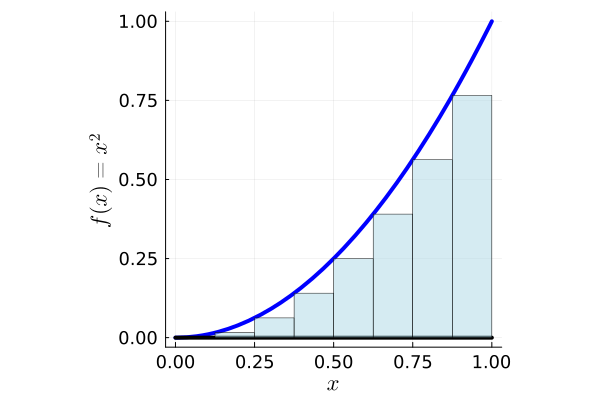
\includegraphics[width=0.45\columnwidth]{graphics/Chap02/AreaParabolaUnderApprox.png}}%
\hspace{5pt}%
\subfloat[]{%
    %\label{fig:MonotonicB}%
	\centering
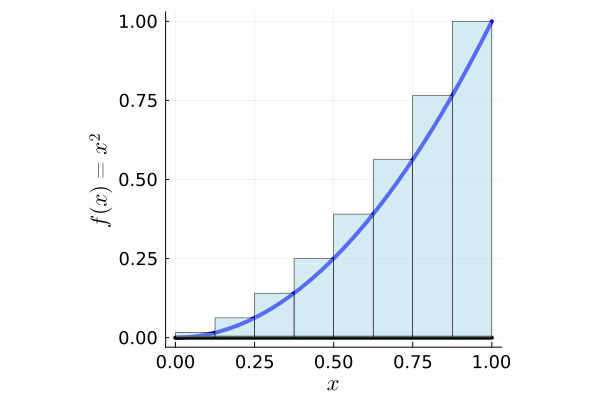
\includegraphics[width=0.45\columnwidth]{graphics/Chap02/AreaParabolaOverApprox.png}}%
    \caption[]{Under- and overapproximations for the area under a parabola. (a) An underapproximation for a parabola defined by $f(x)=x^2,~ 0 \le x \le 1$. (b) An overapproximation for a parabola defined by $f(x)=x^2,~ 0 \le x \le 1$. For (a) and (b), $n=8$ and thus $\Delta x = 0.125$.}
    \label{fig:ApproxAreaParabola}
\end{figure}

\textbf{Area Under a Parabola:} Next, let's carry out our Archimedes-inspired approximation method for $f(x)=x^2$, $a=0$, and $b=1$. Again, with $n>0$, we have $\Delta x =\frac{1}{n}$, $x_i = (i-1) \Delta x$, $f(x_i)= \left((i-1) \Delta x \right)^2$, and 
\begin{equation}
\begin{aligned}
    {\rm Area}^{\rm Low}_n :&=   \sum_{i=1}^n f(x_i)\cdot \Delta x \\
    &=   \sum_{i=1}^n \left((i-1) \Delta x \right)^2 \cdot \Delta x  \\
    &=  \sum_{i=1}^n \left((i-1) \frac{1}{n}\right)^2 \cdot \frac{1}{n} \\
    &= \frac{1}{n^3} \cdot  \sum_{i=1}^n (i-1)^2 ~~~~(\text{because } n \text{ is a constant, we take it out of the sum}) \\
     &= \frac{1}{n^3} \cdot  \sum_{i=1}^{n-1} i^2 ~~~~(\text{change of index}) \\
    &= \frac{1}{n^3} \cdot \frac{(n-1)(n -1 + 1)(2(n-1) + 1) }{6} ~~~~(\text{by Example }\ref{ex:SumIntegersSquared})\\
    & = \frac{1}{n^3} \cdot \frac{2n^3 - 3n^2 + n}{6} \\
    &= \frac{1}{3} - \frac{1}{2n} + \frac{1}{6n^2}.
\end{aligned}
\end{equation}
Similarly, 
\begin{equation}
\begin{aligned}
    {\rm Area}^{\rm Up}_n :&=   \sum_{i=1}^{n} f(x_{i+1})\cdot \Delta x \\
    &=   \sum_{i=1}^n \left(i \Delta x\right)^2 \cdot \Delta x  \\
    &=  \sum_{i=1}^n\left(i \frac{1}{n}\right)^2 \cdot \frac{1}{n} \\
    &= \frac{1}{n^3} \cdot  \sum_{i=1}^n i^2 ~~~~(\text{because } n \text{ is a constant, we take it out of the sum}) \\
    &= \frac{1}{n^3} \cdot \frac{n(n + 1)(2n + 1)}{6}  ~~~~(\text{by Example }\ref{ex:SumIntegersSquared})\\
    &= \frac{1}{n^3} \cdot \frac{2n^3 + 3n^2 + n}{6} \\
    &= \frac{1}{3} + \frac{1}{2n} + \frac{1}{6n^2}.
\end{aligned}
\end{equation}
%n(n + 1)(2n + 1) / 6   .
Hence, for all $n > 1$, 
\begin{equation}
    \label{eqn:AreaparabolaBounds}
    {\rm Area}^{\rm Low}_n =   \frac{1}{3} - \frac{1}{2n} + \frac{1}{6n^2} \le {\rm Area} \le \frac{1}{3} + \frac{1}{2n} + \frac{1}{6n^2} = {\rm Area}^{\rm Up}_n.
\end{equation}
Because $\dfrac{{\rm Area}^{\rm Up}_n + {\rm Area}^{\rm Low}_n }{2} = \dfrac{1}{3} + \dfrac{1}{6n^2} $ and $\dfrac{{\rm Area}^{\rm Up}_n - {\rm Area}^{\rm Low}_n }{2} = \dfrac{1}{n}$, we have
\begin{equation}
    \label{eqn:AreaParabolaApprox}
   \boxed{ {\rm Area}^{\rm est}_n = \left( \frac{1}{3} + \frac{1}{6n^2} \right) \pm \frac{1}{n}.}
\end{equation}
Moreover, as $n$ gets larger and larger, both $\frac{1}{6n^2}$ and $\frac{1}{n}$ become smaller and smaller, leading us to the conclusion that the area under the parabola is $\frac{1}{3}$.

\emstat{
 \textbf{Summary:} To estimate the areas, all we did was add up the areas of a carefully selected set of rectangles. If we were doing the entire thing in Julia, we would not have needed any analytical results at all. We'd have naturally taken $n$ large and obtained lower and upper bounds on our desired quantity. In order to obtain analytical results, all we needed were Examples~\ref{ex:SumFirstIntegersPower1} and \ref{ex:SumIntegersSquared}, which address the sum of the first $n$ integers raised to power ``1'' and power ``2'', respectively. That's a pretty low bar, you have to admit. 

}

\textbf{Area Under under a Triangle and a Parabola, Generalized just a Smidgen}

Instead of computing the areas under the curves over the interval $[0, 1]$, let's consider $[0, x]$, for $x>0$. We won't repeat the steps for the triangle, because the formula $\frac{1}{2} b \cdot h$ still applies, giving us $x^2/2$ for the area. What about the parabola? For the lower bound, with $n>1$ rectangles, we have $\Delta x =\frac{x}{n}$, $x_i = (i-1) \Delta x$, $f(x_i)= \left((i-1) \Delta x \right)^2$, and 
\begin{equation}
\begin{aligned}
    {\rm Area}^{\rm Low}_n :&=   \sum_{i=1}^n f(x_i)\cdot \Delta x \\
    &=   \sum_{i=1}^n \left((i-1) \Delta x \right)^2 \cdot \Delta x  \\
    &=  \sum_{i=1}^n \left((i-1) \frac{x}{n}\right)^2 \cdot \frac{x}{n} \\
    &= \frac{x^3}{n^3} \cdot  \sum_{i=1}^n (i-1)^2 ~~~~(\text{because both } n, x \text{ are independent of } i,\text{ we take them out of the sum}) \\
     &= \frac{x^3}{n^3} \cdot  \sum_{i=1}^{n-1} i^2 ~~~~(\text{change of index}) \\
    &= \frac{x^3}{n^3} \cdot \frac{(n-1)(n -1 + 1)(2(n-1) + 1) }{6} ~~~~(\text{by Example }\ref{ex:SumIntegersSquared})\\
    & = \frac{x^3}{n^3} \cdot \frac{2n^3 - 3n^2 + n}{6} \\
    &= \frac{x^3}{3} - \frac{x^3}{2n} + \frac{x^3}{6n^2}.
\end{aligned}
\end{equation}
When the learner repeats the calculation for the upper bound, they will obtain ${\rm Area}^{\rm Up}_n = \frac{x^3}{3} + \frac{x^3}{2n} + \frac{x^3}{6n^2}$. Combining the lower and upper bounds gives,
\begin{empheq}[box=\bluebox]{equation}
    \label{eqn:AreaParabolaApproxV02}
 {\rm Area}^{\rm est}_n = \left( \frac{x^3}{3} + \frac{x^3}{6n^2} \right) \pm \frac{x^3}{2n}.
\end{empheq}
Moreover, for $x$ fixed (i.e., held constant), as $n$ gets larger and larger, the learner can verify numerically, or via  Fig.~\ref{fig:OneOverNandNsquaredConvergingToZero}, that both $\frac{x^3}{6n^2}$ and $\frac{x^3}{2n}$ become smaller and smaller, leading us to the conclusion that the area under the parabola is $\frac{x^3}{3}$. For $x>0$, the area under the parabola $f(x) = x^2$ for the interval $[0, x]$ is equal to $\frac{x^3}{3}$. In other words, we have a closed-form solution for the area for a general interval $[0, x]$, with very little effort. That's remarkable.

\begin{table}
\centering 
\begin{tabular}{|l|c|c|}
\hline   
Function & Interval & Area \\ \hline 
\hline
$f(x) = x$ & $[0, 1]$ & $1/2$ \\ \hline
$f(x) = x$ & $[0, x]$ & $x^2/2$ \\ \hline 
$f(x) = x^2$ & $[0, 1]$ & $1/3$ \\ \hline 
$f(x) = x^2$ & $[0, x]$ & $x^3/3$ \\ 
\hline
\end{tabular}
\caption{Areas under two simple curves, following a method inspired by Archimedes. The only ``leap of faith'' required so far is that terms of the form $\frac{\text{constant}}{n}$ and $\frac{\text{constant}}{n^2}$ become arbitrarily small (i.e., negligible) as $n$ becomes very large, as illustrated in Fig.~\ref{fig:OneOverNandNsquaredConvergingToZero}.}
\label{tab:FirstIntegrals}
\end{table}

\begin{figure}[htb]%
\centering
\subfloat[]{%
    %
	\centering
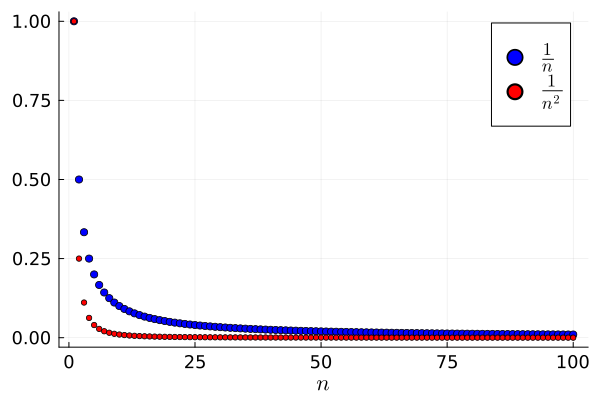
\includegraphics[width=0.75\columnwidth]{graphics/Chap02/OneOverNandNsquaredConvergingToZero.png}}%
    \caption[]{Graphs of $1/n$ and $1/n^2$ versus $n$, for $1 \le n \le 100$.}
    \label{fig:OneOverNandNsquaredConvergingToZero}
\end{figure}

\clearpage

\begin{observationColor}{Ratios of Polynomials of $n$ as $n$ tends to Infinity}{LimitMotivation}

When approximating our areas with a sum of $n$ rectangles, we were faced with terms of the form
\begin{itemize}
    \item Triangle ($f(x) = x$): $\frac{1 + 2 + \cdots + n}{n^2} = \frac{a n^2 + bn}{n^2} $
    \item Parabola ($f(x) = x^2$): $\frac{1^2 + 2^2 + \cdots + n^2}{n^3} = \frac{an^3 + bn^2 + cn}{n^3} $
\end{itemize}
and we can imagine that for the area under $x^k$, $k>2$, we'd be faced with a term of the form  
$$\frac{1^k + 2^k + \cdots + n^k}{n^{k+1}} = \frac{an^{k+1} + bn^k + \cdots + \text{ lower powers of } n }{n^{k+1}}.$$
In each case, we want to let $n$ become large so that our scheme of under- and over-approximations through adding up rectangles becomes more accurate. In the limit, we'd like to take an ``unbounded'' number of ``infinitely thin'' rectangles, which brings us to the notion of ``limits at infinity'', the topic of Chapters~\ref{sec:LimitInfinityHard} and \ref{sec:LimitInfinityEasy}. Before we do that, let's address sums of powers of integers for arbitrary $k \ge 1$.    
\end{observationColor}
% \begin{equation}\label{eqn:SumPowerk}
% \begin{aligned}
%  \sum_{i=1}^{N}i~~ &= \frac{1}{2}(N^2+N)\\
% \sum_{i=1}^{N}i^2 &= \frac{1}{6}(2N^3+3N^2+N)\\
%   \sum_{i=1}^{N}i^3 &= \frac{1}{4}(N^4+2N^3+N^2)\\
%   \sum_{i=1}^{N}i^4 &= \frac{1}{30}(6N^5+15N^4+10N^3-N)\\
%   \sum_{i=1}^{N}i^5 &= \frac{1}{12}(2N^6+6N^5+5N^4-N^2)\\
%   \sum_{i=1}^{N}i^6 &= \frac{1}{42}(6N^7+21N^6+21N^5-7N^3+N)\\
%   \sum_{i=1}^{N}i^7 &= \frac{1}{24}(3N^8+12N^7+14N^6-7N^4+2N^2)\\
%   \sum_{i=1}^{N}i^8 &= \frac{1}{90}(10N^9+45N^8+60N^7-42N^5+20N^3-3N)\\ 
%   \sum_{i=1}^{N}i^9 &= \frac{1}{20}(2N^{10}+10N^9+15N^8-14N^6+10N^4-3N^2)\\ 
%   \sum_{i=1}^{N}i^{10} &= \frac{1}{66}(6N^{11}+33N^{10}+55N^9-66N^7+66N^5-33N^3+5N)  
%   \end{aligned}
%   \end{equation}



\begin{propColor}{Power Sums}{GeneralPowerSums}
For all $n\ge 1$ and $k\ge 1$, the following holds,
% $$ 1^k + 2^k + 3^k + \cdots + n^k =: \sum_{i=1}^{n}i^k =  \frac{n^{k+1}}{k+1} + \frac{n^k}{2} + \bigO(n,k-1),$$
\begin{equation}
    \begin{aligned}
      \sum_{i=1}^{n}i^k :=& 1^k + 2^k + 3^k + \cdots + n^k \\
      =& \frac{n^{k+1}}{k+1} + \frac{n^k}{2} + \bigO(n,k-1),
    \end{aligned}
\end{equation}
where $\bigO(n,k-1)$ stands for a polynomial in the variable $n$ with degree less than or equal to $k-1$ (i.e., all of the lower-order terms after $n^k$).    
\end{propColor}

\begin{rem} 
\label{rem:SamplePowerSums}
If you want to see the explicit values of the sums, here are the first few:
\begin{equation}\label{eqn:SumPowerk}
\begin{aligned}
 \sum_{i=1}^{n}i~~ &= \frac{1}{2}(n^2+n) = \frac{n^2}{2} + \frac{n}{2}\\
\sum_{i=1}^{n}i^2 &= \frac{1}{6}(2n^3+3n^2+n) = \frac{n^3}{3} + \frac{n^2}{2} + \bigO(n,1)\\
  \sum_{i=1}^{n}i^3 &= \frac{1}{4}(n^4+2n^3+n^2) = \frac{n^4}{4} + \frac{n^3}{2} + \bigO(n,2)\\
  \sum_{i=1}^{n}i^4 &= \frac{1}{30}(6n^5+15n^4+10n^3-n) = \frac{n^5}{5} + \frac{n^4}{2} + \bigO(n,3)\\
  \sum_{i=1}^{n}i^5 &= \frac{1}{12}(2n^6+6n^5+5n^4-n^2) = \frac{n^6}{6} + \frac{n^5}{2} + \bigO(n,4).
  \end{aligned}
  \end{equation}   
  You can find longer lists online. A general formula was given by \href{https://en.wikipedia.org/wiki/Faulhaber%27s_formula}{Faulhaber}.
\end{rem}





% \section{Binomial Theorem and its Specializations}

% The binomial theorem states that for any real numbers $x$ and $y$, and any non-negative integer $n$, the expansion of the power $(x + y)^n$ is given by,
% $$(x + y)^n = \sum_{k=0}^{n} \binom{n}{k} x^{n-k}y^k,$$
% where $\binom{n}{k}$, pronounced ``n choose k", denotes the binomial coefficient and is given by.
% $$\binom{n}{k} = \frac{n!}{k!(n-k)!}.$$
% The binomial coefficient $\binom{n}{k}$ gives the number of ways to choose $k$ elements from a set of $n$ elements without regard for the order of selection. Here, $n!$ denotes the factorial of $n$, which is the product of all positive integers up to $n$.

% In the expansion $(x + y)^n$, the $k^{th}$ term is the product of $\binom{n}{k}$, $x^{n-k}$ and $y^k$. Note that the sum of the exponents in each term, $n-k + k$, is always equal to $n$. This reflects the fact that each term corresponds to some way of picking $n-k$ $x$'s and $k$ $y$'s from the $n$ factors in $(x + y)^n$.


% If we specialize the binomial theorem to $(1 + x)^n$, where $x$ is a real number and $n$ is a non-negative integer, we obtain,
% $$(1 + x)^n = \sum_{k=0}^{n} \binom{n}{k} x^k.$$
% In the expansion $(1 + x)^n$, the $k^{th}$ term is the product of $\binom{n}{k}$ and $x^k$. Because we are adding $1$ to $x$, the power of $1$ is $n-k$ in each term, but since $1^{n-k}$ is always $1$, we don't write it out. This results in a simpler expression for the expansion of $(1 + x)^n$.

% A simple upper bound for the binomial coefficient $\binom{n}{k}$ can be given as $n^k/k!$. 
% Indeed, $n!$ is the product of $n$ terms, and for $n \geq k$, there are exactly $k$ terms in the product $n \cdot (n-1) \cdot \ldots \cdot (n-k+1)$ that are greater than or equal to $k$, and thus we have $n! \geq k^k \cdot (n-k)!$. 
% This gives an upper bound for the binomial coefficient $\binom{n}{k}$ as follows,
% $$\binom{n}{k} = \frac{n!}{k!(n-k)!} \leq \frac{k^k (n-k)!}{k!(n-k)!} = \frac{k^k}{k!} \le \frac{n^k}{k!}$$
% for $n \geq k \geq 0$. So, a simple bound for $\binom{n}{k}$ would be $n^k/k!$. This bound, while not always tight, gives a reasonable approximation for the order of magnitude of $\binom{n}{k}$ and is particularly useful for large $n$ and small $k$.

% This is a more straightforward and easy-to-understand bound. More accurate and complicated bounds involve other mathematical concepts and methods, such as Stirling's approximation for the factorial function.

% \section{Euler's Constant Revisited}


% We know from the Binomial Theorem that for any $n \geq 0$,

% \begin{equation}
% (1 + \frac{1}{n})^n = \sum_{k=0}^{n} \binom{n}{k} (\frac{1}{n})^k.
% \end{equation}

% Each term of this sum is non-negative, so the sum is at least as large as each of its terms. This means that for all $n \geq 1$,

% \begin{equation}
% (1 + \frac{1}{n})^n \geq 1,
% \end{equation}

% showing that the sequence is bounded below by 1.

% For the upper bound, we can use the fact that the binomial coefficient $\binom{n}{k}$ is at most $\frac{n^k}{k!}$. This gives us

% \begin{equation}
% (1 + \frac{1}{n})^n = \sum_{k=0}^{n} \binom{n}{k} (\frac{1}{n})^k \leq \sum_{k=0}^{n} \frac{n^k}{k!n^k} = \sum_{k=0}^{n} \frac{1}{k!}.
% \end{equation}

% For all $n \geq 1$, this sum is at most $1 + 1 + \frac{1}{2} + \frac{1}{6} + \frac{1}{24} + \frac{1}{120} + \frac{1}{720} < 3$,

% so the sequence is bounded above by 3.

% Thus, the sequence $(1 + \frac{1}{n})^n$ is bounded as $n$ tends to infinity. This is a rougher bound than using the definition of $e$, but it avoids the need to introduce that concept.


% The series expansion for the exponential function $e^x$ can be obtained from the Taylor series centered at $0$, given by 

% \begin{equation}
% e^x = \sum_{n=0}^{\infty} \frac{x^n}{n!},
% \end{equation}

% which converges for all real numbers $x$.

% In particular, for $x=1$ we obtain the series expansion for the number $e$, which is

% \begin{equation}
% e = \sum_{n=0}^{\infty} \frac{1}{n!}.
% \end{equation}

% It's well-known and can be proved that the number $e$ is approximately $2.71828$ and is indeed less than $3$. 

% But to help students understand why this infinite sum doesn't exceed $3$, let's provide a simpler and more visual argument:

% The sum starts off as $1 + 1 + \frac{1}{2} + \frac{1}{6} + \frac{1}{24} + \frac{1}{120} + \frac{1}{720} + \ldots$, and if we continue this pattern indefinitely, we can see that each subsequent term gets smaller and smaller. 

% Now, let's make an upper bound for each of these terms:

% \begin{equation}
% 1, 1, \frac{1}{2}, \frac{1}{4}, \frac{1}{8}, \frac{1}{16}, \frac{1}{32}, \ldots.
% \end{equation}

% This is the sum of the geometric series with the first term being $1$ and the common ratio being $\frac{1}{2}$. The sum of this series is given by $\frac{a}{1-r} = \frac{1}{1 - 1/2} = 2$, where $a$ is the first term and $r$ is the common ratio.

% Therefore, we can say that the original sum is certainly less than $3$, providing an upper bound without having to resort to calculus or more advanced mathematics. This reasoning can be a good way to help students grasp the idea that the sum of the series is indeed a finite number.

% When we specialize the binomial theorem to $(1 + \frac{1}{n})^n$ with $n$ being a positive integer, we get the following expression:

% $$(1 + \frac{1}{n})^n = \sum_{k=0}^{n} \binom{n}{k} (\frac{1}{n})^k$$

% This becomes:

% $$(1 + \frac{1}{n})^n = \sum_{k=0}^{n} \binom{n}{k} \frac{1}{n^k}$$

% which simplifies to:

% $$(1 + \frac{1}{n})^n = \sum_{k=0}^{n} \frac{n!}{k!(n-k)!n^k}$$

% As $n$ goes to infinity, this series tends towards the number $e$. That's because the sum of the terms from $k=0$ to $k=n$ of $\frac{n!}{k!(n-k)!n^k}$ converges to the sum of the terms of $\frac{1}{k!}$ from $k=0$ to infinity as $n$ goes to infinity, which is the definition of $e$:

% $$e = \sum_{k=0}^{\infty} \frac{1}{k!}$$

% This connection is one of the ways that $e$ is defined and understood.

\section{Limits at Infinity: The Hard Way}
\label{sec:LimitInfinityHard}

Here, we take our first cut at the concept of a limit. We'll first lay out the concept using ``everyday language'', and then we'll formalize it. To make sure we understand the formalization, the examples will be worked in ``excruciating detail''. How's that for encouragement? In compensation, once we really understand what is going on, we'll be able to compute most limits ``by inspection''. 

\begin{tcolorbox}[colback=mylightblue, title = {\bf Finite Limits at $\infty$}, breakable]

\textbf{Conceptual Idea:} Suppose $f:(0,\infty) \to \real$ is a function and $L\in \real$ is a (finite) real number. Then we say \textbf{the limit of $f(x)$ as $x$ approaches infinity equals $L$}, denoted, 
$$ \lim_{x \to \infty} f(x) = L,$$
if we can make $f(x)$ stay ``arbitrarily close'' to $L$ by taking $x$ ``sufficiently large in the positive direction.'' 

\bigskip

The formal definition makes precise what we mean by ``arbitrarily close'' and ``sufficiently large.'' 

\begin{definition}
\label{def:LimitAtInfinity}
(Finite Limit at Infinity) Suppose $f:(0,\infty) \to \real$ is a function and $L\in \real$ is a (finite) real number. Then we say 
$$ \lim_{x \to \infty} f(x) = L$$ 
if, for all $\epsilon >0$ (no matter how small), there exists $N < \infty$, such that, for all $x \ge N$, it holds that $|f(x) - L| \le \epsilon$.\\
\end{definition}

\textbf{Notes:}
\begin{itemize}
    \item for all $x \ge N$ defines ``$x$ sufficiently large''.
    \item $|f(x) - L| \le \epsilon$  defines ``arbitrarily close''. You can think of $\epsilon >0$ as specifying a level of precision. How precisely is $f(x)$ approximated by the constant $L$ for $x$ sufficiently large.
    \item The definition can also be written as: for all $\epsilon >0$, there exists $N < \infty$, such that, $x \ge N \implies |f(x) - L| \le \epsilon$.
    \item It is emphasized that if there is a single point $x \ge N$ such that $|f(x) - L| > \epsilon$, then the ``closeness (aka, precision)'' criterion has failed. We have found a point $x$ where $f(x)$ is not well approximated by the constant $L$. \\
\end{itemize}
 


\textbf{Additional Remarks:}
\begin{itemize}
    \item We note that as we take $\epsilon$ smaller and smaller (aka, our precision requirement becomes finer and finer), we typically need to take $N$ larger and larger. In other words, $N$ typically depends on $\epsilon$. It is sometimes useful to express this dependence as $N(\epsilon)$ or $N_\epsilon$. 

    \item Another way to interpret a limit at infinity is that as we take $N$ larger and larger, the function restricted to $[N, \infty)$ becomes closer and closer to having a constant value equal to $L$.

    \item We will treat the definition of a limit as $x$ approaches $-\infty$ later.  
\end{itemize}


\end{tcolorbox}

\bigskip

 
\begin{example} 
\label{ex:LimitAtPlusInfinity}
Compute $\displaystyle \lim_{x \to \infty} f(x)$, if it exists, for the following functions. 

\begin{enumerate}
\renewcommand{\labelenumi}{(\alph{enumi})}
\setlength{\itemsep}{.2cm}
    \item $f:(0,\infty) \to \real$ by $f(x) = \frac{1}{x}$.
        
    \item $f:(0,\infty) \to \real$ by $f(x) = \frac{1}{x^k}$.
    
    \item $f:\real \to \real$ by $f(x) = \frac{x^2}{1 + 3 x^2}$.
     
     \item $f:\real \to \real$ by $f(x) = \frac{x}{1 + 3 x^2}$.

     % \item $f:\real \to \real$ by $f(x) = \frac{4 x +2}{1 + x^2}$.

\end{enumerate} 

   
\end{example}

\begin{figure}[htb]%
\centering
\subfloat[]{%
    %
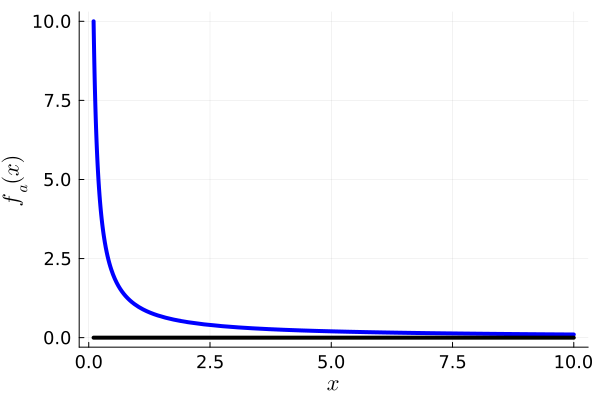
\includegraphics[width=0.45\columnwidth]{graphics/Chap02/ConvergFiniteLimitA.png}}%
\centering
\subfloat[]{%
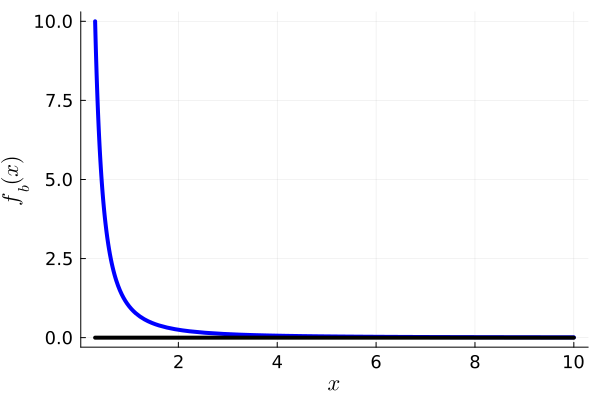
\includegraphics[width=0.45\columnwidth]{graphics/Chap02/ConvergFiniteLimitB.png}}%
\bigskip
\newline
\centering
\subfloat[]{%
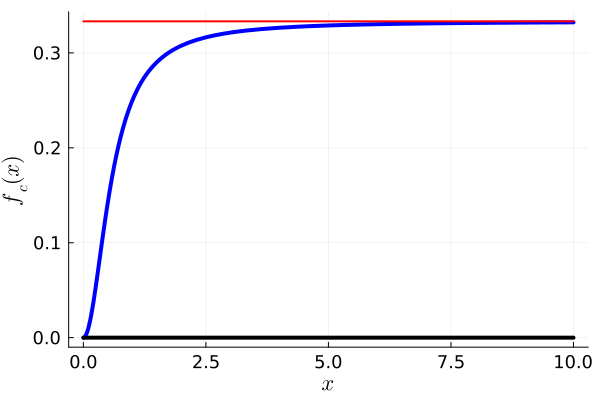
\includegraphics[width=0.45\columnwidth]{graphics/Chap02/ConvergFiniteLimitC.png}}%
\centering
\subfloat[]{%
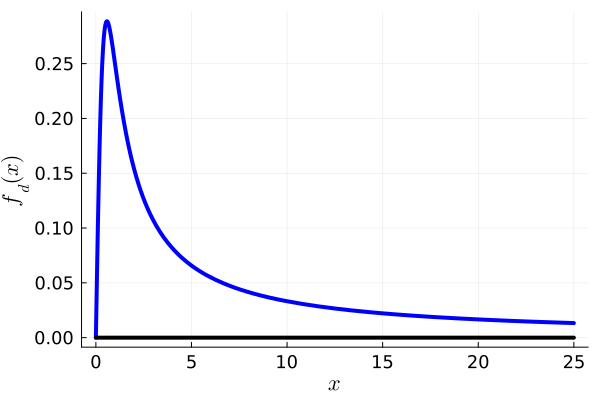
\includegraphics[width=0.45\columnwidth]{graphics/Chap02/ConvergFiniteLimitD.png}}%
% \centering
% \subfloat[]{%
%     %
% 	\centering
% 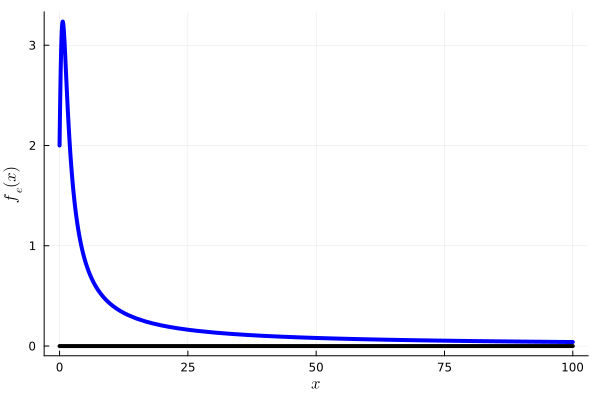
\includegraphics[width=0.45\columnwidth]{graphics/Chap02/ConvergFiniteLimitE.png}}%
    \caption[]{Graphs of the four functions in Example~\ref{ex:LimitAtPlusInfinity}. The red line in (c) shows the non-zero value to which the function is converging.}
    \label{fig:ConvergingToFiniteLimitspart01}
\end{figure}

\textbf{Solutions:}

\begin{enumerate}
\renewcommand{\labelenumi}{(\alph{enumi})}
\setlength{\itemsep}{.3cm}
    \item $f(x) = \frac{1}{x}$ for $x > 0$. \Ans $\displaystyle\lim_{x \to \infty} f(x) =0.0$\\
    
 To show this, set $L=0.0$ and choose $\epsilon >0$ but otherwise arbitrary. Then for all $x > \frac{1}{\epsilon}$, we have 
$$ |f(x) -L| = | \frac{1}{x} - 0.0|  = \frac{1}{x} < \frac{1}{\frac{1}{\epsilon}} = \epsilon,  $$
where we used $\frac{1}{x} =\frac{1}{\text{a bigger number}} < \frac{1}{\text{a smaller number}} = \frac{1}{\frac{1}{\epsilon}}$, when $\boxed{x > \frac{1}{\epsilon}}$.


\textbf{Note:} Because $N(\epsilon) := \frac{1}{\epsilon}$, when $\epsilon$ becomes small to bound $|f(x) -L|$, we have at the same time $N(\epsilon)=\frac{1}{\epsilon}$ becoming large, imposing that $x > N$ is large. 


      \item $f(x) = \frac{1}{x^k}$ for $x > 0$.   \Ans $\displaystyle\lim_{x \to \infty} f(x) =0.0$.\\

       To show this, set $L=0.0$ and choose $\epsilon >0$ but otherwise arbitrary. Then for all $x > \frac{1}{\sqrt[k]{\epsilon}}$, we have 
$$ |f(x) -L| = | \frac{1}{x^k} - 0.0|  = \frac{1}{x^k} < \frac{1}{\left(\frac{1}{\sqrt[k]{\epsilon}}\right)^k} = \frac{1}{\frac{1}{\epsilon}} = \epsilon .  $$

\textbf{Notes:} The remarks from the previous problem apply here, with the exception that $N(\epsilon):= \frac{1}{\sqrt[k]{\epsilon}}$. It is still true that $\epsilon$ small forces $N(\epsilon)$ to be large.

    
    \item $f:\real \to \real$ by $f(x) = \frac{x^2}{1 + 3 x^2}$. \Ans $\displaystyle\lim_{x \to \infty} f(x) =\frac{1}{3}$.\\

    To show this, set $L=1/3$ and choose $\epsilon >0$ but otherwise arbitrary. We rewrite the function as, for all $x \neq 0$,
    $$f(x) = \frac{x^2}{1 + 3 x^2} \cdot \frac{\frac{1}{x^2}}{\frac{1}{x^2}} =  \frac{1}{\frac{1}{x^2} + 3 }.$$
     Then, 
   $$ |f(x) -L| = |\frac{1}{\frac{1}{x^2} + 3 } - \frac{1}{3}|  =  \frac{1}{3} - \frac{1}{\frac{1}{x^2} + 3 }.$$ 
   Now, let's set $\delta =  \frac{1}{x^2}$ and solve for $\delta>0$ such that $\frac{1}{3} - \frac{1}{\delta + 3 } < \epsilon.$ Hence, after some algebra (nothing to do with Calculus), we work out
   $$\frac{1}{3} - \frac{1}{\delta + 3 } = \frac{\delta}{3 (\delta + 3)} < \epsilon \iff \delta < 3 \epsilon (\delta + 3) \iff (1-3 \epsilon) \delta < 9 \epsilon .$$
   Because $(1-3 \epsilon) < 1$ for all $\epsilon>0$, we have that  $(1-3 \epsilon) \delta < \delta$, and 
   $$\delta < 9 \epsilon \implies   |\frac{1}{\delta + 3 } - \frac{1}{3}| < \epsilon. $$ 
   Hence, replacing $\delta$ by $\frac{1}{x^2}$, we have that  $\frac{1}{x^2} < 9 \epsilon  \implies |\frac{1}{\frac{1}{x^2} + 3 } - \frac{1}{3}|  < \epsilon$, from which we deduce that
   $$ x> \frac{1}{3 \sqrt{\epsilon}} \implies |\frac{1}{\frac{1}{x^2} + 3 } - \frac{1}{3}| < \epsilon,$$ 
   and hence we have shown that $\displaystyle\lim_{x \to \infty} f(x) =\frac{1}{3}$. 

\emstat{
   \textbf{Notes:}
\begin{itemize}
\item The above is what computing limits by hand typically looks like: \textcolor{red}{\bf a blaze of symbols, multiple lines of computations, each of which is a likely opportunity for making errors}. 
    \item While in this example, the messy algebra and bounding of terms was actually done back in Example~\ref{ex:ManipulatingInequalities02}, there is no way you would have remembered that!
    \item \textbf{Bottom line:} Finding situations where we could write down the limits by inspection, while avoiding the messy algebra, would be nice. We will do that shortly.
\end{itemize}
}


     \item $f(x) = \frac{x}{1 + 3 x^2}$ \Ans $\displaystyle\lim_{x \to \infty} f(x) =0.0$.\\


     To show this, set $L=0.0$ and choose $\epsilon >0$ but otherwise arbitrary. We rewrite the function as, for all $x \neq 0$,
    $$f(x) = \frac{x}{1 + 3 x^2} \cdot \frac{\frac{1}{x}}{\frac{1}{x}} =  \frac{1}{\frac{1}{x} + 3x }.$$
    Then, for all $x>0$,
   $$ |f(x) -L| = | \frac{1}{\frac{1}{x} + 3x } - 0.0|  < \frac{1}{0 + 3x }.$$ 
   We observe that 
   $$\frac{1}{3x } < \epsilon \iff 3x > \frac{1}{\epsilon} \iff x > \frac{1}{3\epsilon}.$$ 
   Hence, here, $N(\epsilon) =\frac{1}{3\epsilon}.$\\

  There is more than one way to make these estimates. For example, if we had instead written, for all $x > 0$,
    $$f(x) = \frac{x}{1 + 3 x^2} \cdot \frac{\frac{1}{x^2}}{\frac{1}{x^2}} =  \frac{\frac{1}{x}}{\frac{1}{x^2} + 3 },$$
    then, for all $x>1$,
   $$ |f(x) -L| = | \frac{\frac{1}{x}}{\frac{1}{x^2} + 3 } - 0.0|  < \frac{\frac{1}{x}}{0 + 3 }= \frac{1}{3x},$$ 
   yielding the same result we had before.

   % \item $f(x) = \frac{4 x +2}{1 + x^2}$. \Ans $\displaystyle\lim_{x \to \infty} f(x) =0.0$.\\

   % To show this, set $L=0.0$ and choose $\epsilon >0$ but otherwise arbitrary. We rewrite the function as, for all $x \neq 0$,
   %  $$f(x) = \frac{4 x +2}{1 + x^2}\cdot \frac{ \frac{1}{x^2} }{ \frac{1}{x^2} } =  \frac{ \frac{4}{x} + \frac{2}{x^2} }{ \frac{1}{x^2} + 1 }.$$
   %  Then, for all $x>0$,
   % $$ |f(x) -L| = |  \frac{ \frac{4}{x} + \frac{2}{x^2} }{ \frac{1}{x^2} + 1 } - 0.0|  < \frac{\frac{6}{x}}{0 + 1 } = 6 \cdot \frac{1}{x}.$$ 
   % We observe that 
   % $$\frac{6 }{x } < \epsilon \iff x > \frac{6}{\epsilon}.$$ 
   % Hence, here, $N(\epsilon) =\frac{6}{\epsilon}.$\\
   

\end{enumerate} 

\Qed

\bigskip

\emstat{\textbf{Strategy for Bounding Ratios of Functions:} To find an upper bound for a fraction, $\frac{n(x)}{d(x)}$, you replace the numerator with an upper bound and the denominator with a lower bound for the inequality to hold. In symbols, suppose that $0 \le n(x) \le N(x)$. Then, 
$$\frac{n(x)}{d(x)} \le \frac{N(x)}{d(x)},$$ \\
because having a larger number in the numerator gives a larger fraction. 
Next, suppose that $0 < D(x) \le d(x)$. Then, 
$$\frac{n(x)}{d(x)} \le \frac{N(x)}{d(x)} \le \frac{N(x)}{D(x)} ,$$ 
because having a smaller number in the denominator yields a larger fraction. \textbf{While these are ``obvious'' facts, applying them successfully when you are first learning limits can be hard to master!}\\

\textbf{Conversely, to find a lower bound for a fraction}, $\frac{n(x)}{d(x)}$, you replace the numerator with a lower bound and the denominator with an upper bound for the inequality to hold. \\

In other words, if $n(x) \ge N(x)$ and $0 < d(x) \le D(x) $, then $\frac{n(x)}{d(x)} \ge \frac{N(x)}{D(x)}$. This is useful for showing a limit is equal to infinity.}


\bigskip


\begin{tcolorbox}[colback=mylightblue, title = {\bf Infinite Limit at $\infty$}, breakable]

\textbf{Conceptual Idea:} A function $f:(0, \infty) \to \real$ converges to infinity as $x$ tends to $\infty$ if for all finite values of $L$, ``$f(x)$ eventually equals or exceeds $L$ and does not drop below $L$''. 

\bigskip

The formal definition makes precise what we mean by `` eventually equals or exceeds $L$ and does not drop below it.''

\begin{definition}
\label{def:LimitAtInfinity02}
(Unbounded Limits at Infinity) The function $f:(0,\infty) \to \real$ has an \textbf{unbounded positive limit at infinity} if, for every finite $L>0$, there exists $N< \infty$ such that,  
$$x\ge N \implies f(x) \ge L, $$
that is, for all $x \in [N, \infty)$, $f(x)\ge L$. We emphasize that there cannot be any $x \in [N, \infty)$ such that $f(x)< L$; the function has to exceed or equal $L$ and not drop below it. \\

The function $f:(0,\infty) \to \real$ has an \textbf{unbounded negative limit at infinity} if, for every finite $L<0$, there exists $N< \infty$ such that,  
$$x \ge N \implies f(x) \le L, $$
that is, for all $x \in [N, \infty)$, $f(x)\le L$. We emphasize that there cannot be any $x \in [N, \infty)$ such that $f(x)> L$; the function has to be less than or equal to $L$ and not rise above it. \\

We denote these limits by  $\displaystyle\lim_{x \to \infty} f(x) = \infty$ and $\displaystyle\lim_{x \to \infty} f(x) = -\infty$, respectively. 
\end{definition}

\textbf{Note:} For the definition of $\displaystyle\lim_{x \to \infty} f(x) = -\infty$, you may be worried that $L<0$ does not ``look big and negative''. However, $L=-10^9$ is big and negative. We allow $L$ to be any negative real number.

\end{tcolorbox}

\bigskip

\begin{example} 
\label{ex:UnboundedLimitAtPlusInfinity}
Compute $\displaystyle \lim_{x \to \infty} f(x)$, if it exists, for the following functions. 

\begin{enumerate}
\renewcommand{\labelenumi}{(\alph{enumi})}
\setlength{\itemsep}{.2cm}
     \item  $f:\real \to \real$ by $f(x) = \frac{20 x^3 + 11 x^2 + 14}{1 + x^2}$.
        \item   $f:\real \to \real$ by $f(x) = -x^3$.
    \item  $f:\real \to \real$ by $f(x) = x \cdot \sin(x)$.
    \item  $f:\real \to \real$ by $f(x) = \frac{-4x^3 + 11 x + 14}{1 + x^4}$.
\end{enumerate} 
    
\end{example}


    \begin{figure}[htb]%
\centering
\subfloat[]{%
    %
	\centering
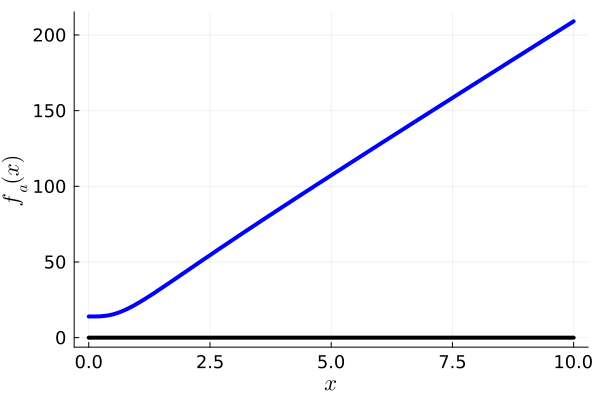
\includegraphics[width=0.45\columnwidth]{graphics/Chap02/ConvergingToInfinityA.png}}%
\hspace{5pt}%
\subfloat[]{%
    %\label{fig:MonotonicB}%
	\centering
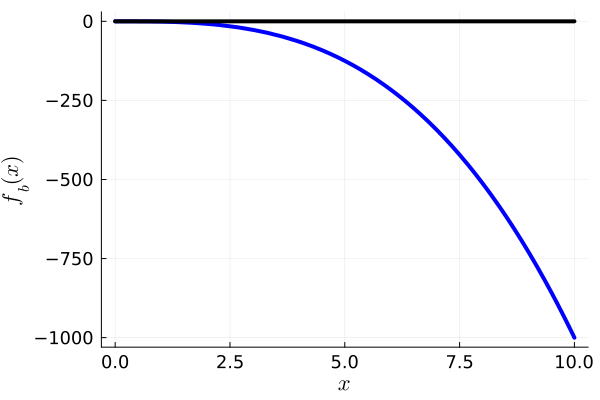
\includegraphics[width=0.45\columnwidth]{graphics/Chap02/ConvergingToInfinityB.png}}%
\hspace{5pt}%
\subfloat[]{%
    %\label{fig:MonotonicB}%
	\centering
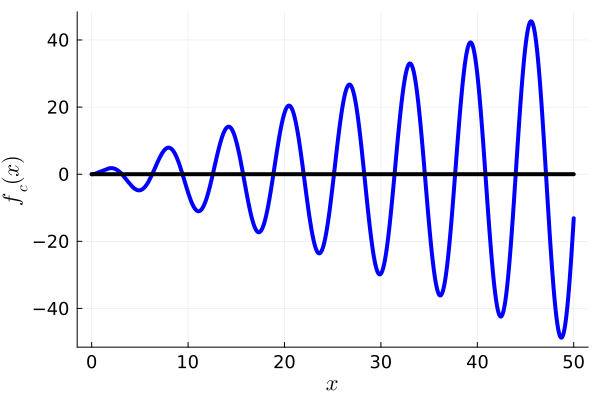
\includegraphics[width=0.45\columnwidth]{graphics/Chap02/ConvergingToInfinityC.png}}%
\hspace{5pt}%
\subfloat[]{%
    %\label{fig:MonotonicB}%
	\centering
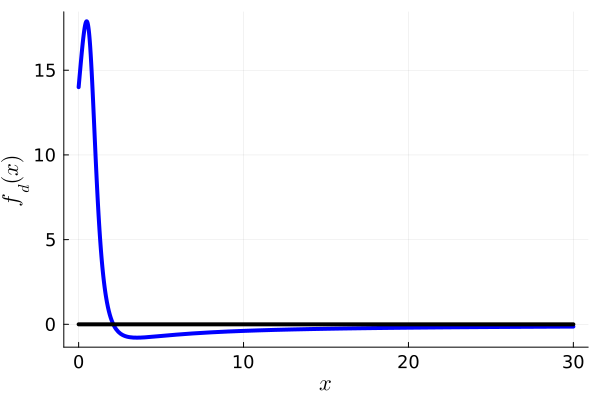
\includegraphics[width=0.45\columnwidth]{graphics/Chap02/ConvergingToInfinityD.png}}%
    \caption[]{Graphs of the four functions in Example~\ref{ex:UnboundedLimitAtPlusInfinity} The plot of $x \cdot \sin(x)$ given in (c) shows that the function becomes unbounded without converging to anything, not even infinity.}
    \label{fig:LimitsAtInfinity}
\end{figure}

\textbf{Solutions:}

\begin{enumerate}
\renewcommand{\labelenumi}{(\alph{enumi})}
\setlength{\itemsep}{.3cm}
    
\item $f(x) = \frac{20 x^3 + 11 x^2 + 14}{1 + x^2}$. \Ans $\displaystyle\lim_{x \to \infty} f(x) =  \infty$.\\

To show this, we first rewrite the function as we have done several times before, for $x>1$,
$$f(x) = \frac{20 x^3 + 11 x^2 + 14}{1 + x^2} =  \frac{20 x^3 + 11 x^2 + 14}{1 + x^2} \cdot  \frac{\frac{1}{x^2}}{\frac{1}{x^2}} = \frac{20 x + 11 + \frac{14}{x^2}}{\frac{1}{x^2} + 1}\ge \frac{20 x + 11}{1 + 1}\ge 10 x.$$
Next, let $L>0$ be otherwise arbitrary and let $ N \ge L/10$. Then, for all $x \ge N$, $f(x) \ge L. $

 \item  $f(x) = -x^3$. \Ans $\displaystyle\lim_{x \to \infty} f(x) = - \infty$.\\

 To show this, let $ L < -1$ be otherwise arbitrary and set $N=|L|$. Then $x > N \implies f(x) = -x^3 < - N^3 <-|L|^3 < L$. You could also have taken $N=\sqrt[3]{|L|}$ and made similar estimates. All that matters is that you show that you find a region of $[N, \infty) \subset \real$ such that $f(x) \le L$ for $x\in [N, \infty)$.

\item $f(x) = x \cdot \sin(x)$. \Ans $\displaystyle\lim_{x \to \infty} f(x)$ does not exist.\\

The issue is that $x\cdot \sin(x)$ becomes arbitrarily large in both the positive direction and the negative direction as $x \to \infty$. To show this, we first note that
$$ \sin(x) = \begin{cases} +1 & x = \frac{\pi}{2} + 2k \pi, k \in \nat \\   -1 & x = -\frac{\pi}{2} + 2k \pi, k \in \nat,\end{cases}$$
where we used the $+1$ to emphasize the positive value. Hence, for arbitrary $L$ and $N>0$, taking $k=\max\{|L|, N\}$ results in $f(\frac{\pi}{2} + 2k \pi) = \frac{\pi}{2} + 2k \pi > L$ and  $f(-\frac{\pi}{2} + 2k \pi) = \frac{\pi}{2} - 2k \pi < L$. We cannot make the function stay above $L$ or below $L$ for all $x > N$.

\item $f(x) = \frac{-4x^3 + 11 x + 14}{1 + x^4}$. \Ans $\displaystyle\lim_{x \to \infty} f(x) =  0$.\\

To show this, we first rewrite the function as we have done several times before, for $x>1$,
$$f(x) = \frac{-4x^3 + 11 x + 14}{1 + x^4} =  \frac{-4x^3 + 11 x + 14}{1 + x^4} \cdot  \frac{\frac{1}{x^4}}{\frac{1}{x^4}} = \frac{-4\frac{1}{x} + 11 \frac{1}{x^3}  + 14 \frac{1}{x^4} }{\frac{1}{x^4} + 1}.$$
Next, let $L=0$ and for all $x>1$, 
$$ |f(x) - L| = |f(x)-0| =  \frac{|-4\frac{1}{x} + 11 \frac{1}{x^3}  + 14 \frac{1}{x^4} |}{|\frac{1}{x^4} + 1|}\le \frac{1}{x} \frac{|4 + 11  + 14  |}{0 + 1} \le  29 \frac{1}{x} . $$
Hence, for all $x > \frac{29}{\epsilon}>1$, $|f(x) -0| \le \epsilon$, which shows that the limit is zero.
\end{enumerate}

\Qed



\bigskip


\begin{tcolorbox}[colback=mylightblue, title = {\bf Neither Finite nor Infinite Limit at $\infty$ Exists}, breakable]

We need to work out what it means to fail a definition. If you are super good at logic, all you have to do is negate the definition! At this stage of your mathematics education, that is easier said than done, so we'll take it step by step. The main mental hurdle is that a definition typically requires several conditions to hold, and hence it fails if any ONE OF THEM does not hold. Logically, this arises from the negation of ``and'' being ``or''. For example, if we have \textbf{MyDef is True} if \textbf{P1} and \textbf{P2} (both) hold, then  \textbf{MyDef is False} if either of \textbf{P1} or \textbf{P2} does not hold. \\

\textbf{Conceptual Ideas:} We say that $f:(0, \infty) \to \real$ \textbf{does not have a finite limit} as $x$ tends to infinity if, for all candidate finite limits $L$, it is impossible to ensure that $f(x)$ remains near $L$ by taking $x$ sufficiently large. Similarly, $f(x)$ does not converge to infinity if for some finite $L>0$, the function keeps ``dipping'' below $L$. 



\bigskip

The formal anti-definitions clarify what ``impossible to keep $f(x)$ near $L$'' or ``dipping below $L$'' really mean!

\begin{definition}
\label{def:NoFiniteLimitAtInfinity}
(No Finite Limit at Infinity) Suppose $f:(0, \infty) \to \real$ is a function. Then $f(x)$ does not have a finite limit at infinity if for every choice of $L \in \real$, there exists some $\epsilon>0$ such that one of the following hold:
    \begin{itemize}
        \item  there does not exist $N < \infty$ so that $x > N \implies |f(x)-L| < \epsilon$.
     \item  for all $N < \infty$ no matter how large, it is not true that $x > N \implies |f(x)-L| < \epsilon$.
    \item  for all $N < \infty$ no matter how large, there (always) exists some $x > N$ such that $|f(x)-L| \ge \epsilon$.
    \end{itemize}
\end{definition}

The last three statements are all equivalent. We have simply ``unwrapped'' the negations one by one. They all capture the idea that ``for every choice of $L \in \real$, we are unable to keep the function's values near $L$ by taking $x$ sufficiently large''. The notion of ``$f(x)$ is not near $L$'' is codified by the existence of some positive value $\epsilon$ being used to bound the ``distance of $f(x)$ from $L$,'' via $|f(x)-L| \ge \epsilon$. \\

\begin{definition}
\label{def:InfiniteLimitAtInfinity}
(No Infinite Limit at Infinity) Suppose $f:(0, \infty) \to \real$ is a function. Then $f(x)$ does not have an unbounded limit at infinity in the positive direction if for some choice of $L >0 $ and every choice of $0< N_L < \infty$ (no matter how large), there exists $x \ge N_L$ such that $f(x) \le L$. Similarly, $f(x)$ does not have an unbounded limit at infinity in the negative direction if for some choice of $L < 0 $ and every choice of $0< N_L < \infty$ (no matter how large), there exists $x \ge N_L$ such that $f(x) \ge L$.\\

\textbf{Classic Example} is shown in Fig.~\ref{fig:LimitsAtInfinity}-(c). Yes, the function grows without bound, but it fails to stay large in the positive direction (or alternatively, the negative direction), as do the curves in Fig.~\ref{fig:LimitsAtInfinity}-(a) and -(b). 
    

\end{definition}
    
 
\end{tcolorbox}

\begin{figure}[htb]%
\centering
\subfloat[]{%
    %
	\centering
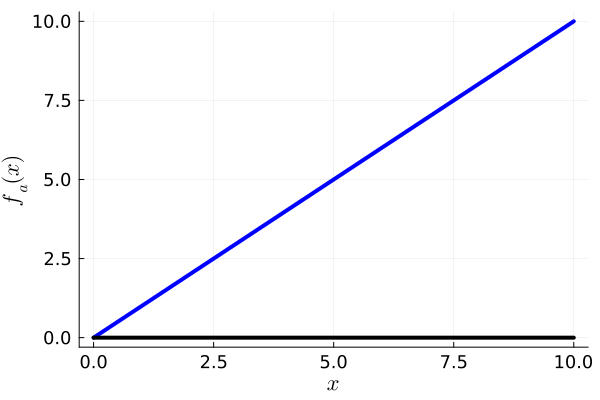
\includegraphics[width=0.3\columnwidth]{graphics/Chap02/ConvergingToFiniteLimit2A.png}}%
\hspace{5pt}%
\centering
\subfloat[]{%
    %
	\centering
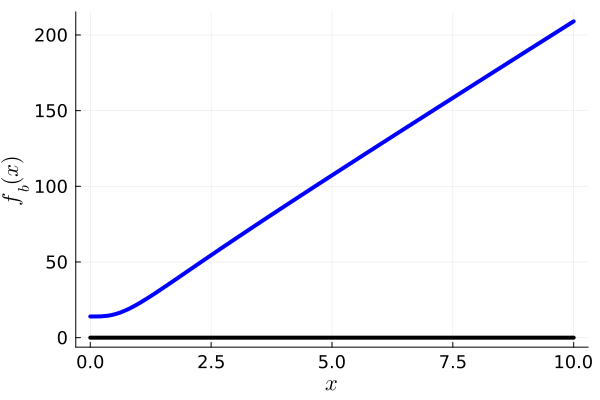
\includegraphics[width=0.3\columnwidth]{graphics/Chap02/ConvergingToFiniteLimit2B.png}}%
\centering
\subfloat[]{%
    %
	\centering
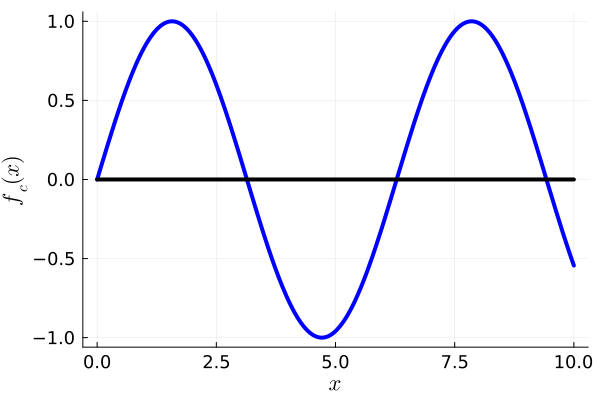
\includegraphics[width=0.3\columnwidth]{graphics/Chap02/ConvergingToFiniteLimit2C.png}}%
    \caption[]{Graphs of the three functions in Example~\ref{ex:LimitAtPlusInfinity02}.}
    \label{fig:ConvergingToFiniteLimitspart2}
\end{figure}

\bigskip


\begin{example} 
\label{ex:LimitAtPlusInfinity02}
Compute $\displaystyle \lim_{x \to \infty} f(x)$, if a finite limit exists for the following functions. 

\begin{enumerate}
\renewcommand{\labelenumi}{(\alph{enumi})}
\setlength{\itemsep}{.2cm}
    \item   $f:\real \to \real$ by $f(x) = x$.
     \item  $f:\real \to \real$ by $f(x) = \frac{20 x^3 + 11 x + 14}{1 + x^2}$.
    \item  $f:\real \to \real$ by $f(x) = \sin(x)$.
\end{enumerate} 
    
\end{example}

\textbf{Solutions:}

\begin{enumerate}
\renewcommand{\labelenumi}{(\alph{enumi})}
\setlength{\itemsep}{.3cm}
    \item $f(x) = x$ does not have a finite limit as $x$ becomes arbitrarily large. While this seems patently obvious, how would one actually show it? 
    
    \begin{itemize} 
    
    \item Solution 1: We use Condition 1 of our ``anti-definition'', namely, for every choice of $L \in \real$, and for every choice of $N < \infty$, there is always an $ x>N$ such that $f(x) > L$. This is easy to show because we can let $L\in \real$ and $0< N < \infty$ be arbitrary. Then for $x > \max\{L, N\}$, $f(x) = x >L$. 
    
    \item Solution 2: We use Condition 4 of our  ``anti-definition'', namely,  for every choice of $L \in \real$, there exists some $\epsilon>0$ such that, for all $N < \infty$ no matter how large, there (always) exists some $x > N$ such that $|f(x)-L| \ge \epsilon$. To show this, let $L$ be arbitrary and choose $\epsilon = 1$. Then, for all $x > L + \epsilon $,
    $$  |x - L| = x - L > L + \epsilon - L =  \epsilon. $$
   Hence, no matter what $L$ we choose, and for all $N$ finite, we have $x > \max\{N, L+ \epsilon\} \implies |f(x) - L| \ge \epsilon$. \\

    \end{itemize}

    
    \textbf{Note:} Yes, it seems clear that $\lim_{x \to \infty} x = \infty$ and we will formalize that shortly. 


    \item  $f(x) = \frac{20 x^3 + 11 x + 14}{1 + x^2}$ does not have a finite limit as $x$ becomes arbitrarily large. We observe that the numerator is growing at ``rate'' $x^3$, while the denominator is growing at rate $x^2$. Hence, the numerator should ``win''. How do we formalize this? Let's rewrite, for all $x \ne 0$, 
    $$\frac{20 x^3 + 11 x + 14}{1 + x^2} = \frac{20 x^3 + 11 x + 14}{1 + x^2} \cdot \frac{\frac{1}{x^2}}{\frac{1}{x^2}} =\frac{20 x + \frac{11}{x} + \frac{14}{x^2}}{\frac{1}{x^2} + 1} .$$
    Then, for all $x> 1$,
    $$f(x) = \frac{20 x + \frac{11}{x} + \frac{14}{x^2}}{\frac{1}{x^2} + 1} > \frac{20 x }{1 + 1} \ge 10 x ,$$
    which grows unbounded as $x$ tends to infinity, meaning, there is no finite limit.

    \item $f(x) = \sin(x)$ has no limit as $x \to \infty$ because no matter how large $N$ becomes,  $\sin:[N, \infty) \to \real$ still oscillates between $-1$ and $1$. While that really is ``enough said'', let's be stubborn and spell out all the details. 
    \begin{enumerate}
        \item Case 1: The candidate limit $L \notin [-1, 1]$ and hence $|L| > 1$. Let $\delta =|L|-1>0$. For all $y\in [-1, 1]$, it follows that $|y|\le1$ and hence $|~|L|-|y|~| \ge \delta$. By the reverse triangle inequality in Prop.~\ref{thm:triangleAndReverseTriangleInequality}, we have $|L-y| \ge \delta$. Hence, for all $\epsilon \le \delta$ and $x \in \real$, $|L - \sin(x)|=|\sin(x)-L| > \delta \ge \epsilon$, and thus $L$ cannot be a limit.

        \item Case 2: The candidate limit $L=0$. Then for $\epsilon = 0.5$ and for all $N< \infty$,  it follows that $x = N \frac{\pi}{2}$ satisfies $x > N$ and $|\sin(x)-L|=|1 - 0| = 1 > 0.5 = \epsilon$, and hence $L$ is not a limit. 
        
        \item Case 3: The candidate limit $L\in [-1, 1]$ and $L \neq 0$. Then there exists $x\in[-\pi, \pi]$ such that $f(x)=L$ and $f(-x)=-L$. Moreover, because $\sin(-x + 2 k \pi) = \sin(-x) = -\sin(x)$, we have that $f(-x + 2 k \pi)=-L$. Hence, we can take $\epsilon = |L|>0$ and note that for all $1<N < \infty$, $-x + 2N \pi > N$ and $|f(-x + 2N \pi) - L| = |\sin(-x + 2N \pi)-L| =  |\sin(-x)-L| = 2|L|>\epsilon$.
    \end{enumerate}

\end{enumerate}

\Qed

\bigskip



\begin{funColor}{Why Do We Care About Limits Anyway?}{CaringAboutLimits}
Limits seem hard. Can't Calculus exist without them? 

\begin{enumerate}
\item \textbf{Limits are the Building Blocks of Calculus:}  Calculus without limits is like a castle floating in the air. Limits are the bedrock of this mathematical fortress.
\item \textbf{Infinity Demystified:} Limits turn the concept of infinity from a perplexing puzzle into a manageable marvel, allowing us to reason about the infinitely small and large.
\item \textbf{Solving the Unsolvable:} Limits provide a method to solve problems that might otherwise be unsolvable. For example, they can be used to determine the value of a function at a point where it's undefined. To see what this might mean, what values should we assign at ...
\begin{itemize}
\item $x=1$ for $\frac{x^3 - 6x^2 + 11x - 6}{x-1}$ (were we not taught to NEVER divide by zero)?
\item $t=0$ for $\frac{\sin(t)}{t}$ (shows up in Signal Processing when building low-pass filters)?
\item $h=0$ for $\frac{e^h-1}{h}$ (rate of change of the natural exponential at the origin)?
\item $n \to \infty$ for $\frac{n^2 + n}{2n^2}$ (area under a unit parabola between zero and one)?
\item $t \to \infty$ for $t \cdot e^{-t} \cdot \sin(3t)$ (infinity times zero times an oscillation)? Shows up in feedback control!
\end{itemize}

\end{enumerate}
    
\end{funColor}

\section{Limits at Infinity: The Easy Way}
\label{sec:LimitInfinityEasy}

Now that we've computed limits by the book, we can make a few observations and profit from them. 

\subsection{Rational Functions}
\label{sec:EasyLimitsRationalFunctions}
In Examples~\ref{ex:LimitAtPlusInfinity}, \ref{ex:LimitAtPlusInfinity02}, and 
\ref{ex:UnboundedLimitAtPlusInfinity}, we had many \textbf{rational functions}, that is, functions consisting of the ratio of two polynomials. Recall that the 
\textbf{degree of a polynomial (aka, ``order'' of the polynomial)} is the highest power of the variable in the polynomial expression. The coefficient multiplying the term of the highest degree is called the \textbf{leading coefficient}; by definition, it cannot be zero. In all of our examples, the nature of the limit of a rational function could be determined by degrees of the numerator and denominator polynomials, and their corresponding leading coefficients. \textbf{Goodbye, tedious calculations!} \\

\emstat{
\textbf{Intuition for the limit of a rational function of $x$:} With a little algebra, we can rewrite a general rational function of $x$ as:

$$\frac{b_m x^m + b_{m-1} x^{m-1} +  \cdots + b_0}{a_n x^n + a_{n-1} x^{n-1} +  \cdots + a_0} = \boxed{\frac{x^m }{x^n}} \cdot \frac{b_m + b_{m-1} \frac{1}{x} +  \cdots + b_0 \frac{1}{x^m}}{a_n  + a_{n-1} \frac{1}{x} +  \cdots + a_0 \frac{1}{x^n}}.$$

 % \boxed{ \frac{x^m }{x^n} \cdot \frac{b_m }{a_n} } \cdot \frac{1 + \frac{b_{m-1}}{b_m} \cdot \frac{1}{x} +  \cdots + \frac{b_0}{b_m} \cdot \frac{1}{x^m} }{1  + \frac{a_{n-1}}{a_n} \frac{1}{x} +  \cdots + \frac{a_0}{a_n} \frac{1}{x^n} }

Because all terms of the form $\frac{1}{x^k}$ go to zero as $|x|$ tends to infinity, the ``messy fraction'' on the right has a simple limit, namely,
$$
\lim_{x \to \pm \infty} ~~  \frac{\bm{b_m} + b_{m-1} \frac{1}{x} +  \cdots + b_0 \frac{1}{x^m}}{\bm{a_n}  + a_{n-1} \frac{1}{x} +  \cdots + a_0 \frac{1}{x^n}} = \boxed{ \frac{b_m }{a_n}}. 
$$
Hopefully, you see it. If not, play with the limit in Julia. Once we have replaced the messy term, $$ \frac{b_m + b_{m-1} \frac{1}{x} +  \cdots + b_0 \frac{1}{x^m}}{a_n  + a_{n-1} \frac{1}{x} +  \cdots + a_0 \frac{1}{x^n}}, $$
with the constant $ \frac{b_m }{a_n}$, all we need to do is understand 
$$\lim_{x \to \pm \infty}  ~~ \frac{b_m }{a_n}  \cdot \frac{x^m }{x^n} = \frac{b_m }{a_n}  \cdot \lim_{x \to \pm \infty}  ~~  \frac{x^m }{x^n},$$
which seems ``infinitely easier''!  
\textbf{This is Prop.~\ref{thm:EasyLimitRationalFunctions} in a nutshell.}
}

\bigskip

\begin{propColor}{Limit of a Rational Function as $x$ tends to Plus or Minus Infinity}{EasyLimitRationalFunctions}
Consider a rational function 
$$\frac{b_m x^m + b_{m-1} x^{m-1} +  \cdots + b_0}{a_n x^n + a_{n-1} x^{n-1} +  \cdots + a_0},$$
where $b_m$ and $a_n$ are non-zero. Then the limit as $x$ tends to plus or minus infinity is equal to
\begin{equation}
\label{eq:EasyLimitsRationalFunctionPlusMinusInfinity}
 \lim_{x \to \pm \infty}  \frac{b_m x^m + b_{m-1} x^{m-1} +  \cdots + b_0}{a_n x^n + a_{n-1} x^{n-1} +  \cdots + a_0} =  \frac{b_m }{a_n} \cdot  \lim_{x \to \pm \infty}   x^{m-n}.
\end{equation}
In particular, 
\begin{equation}
\label{eq:EasyLimitsRationalFunctionPlusInfinity}
    \lim_{x \to \infty}  \frac{b_m x^m + b_{m-1} x^{m-1} +  \cdots + b_0}{a_n x^n + a_{n-1} x^{n-1} +  \cdots + a_0} = \begin{cases}
        \sign\left( \frac{b_m }{a_n}  \right) \cdot \infty & m > n \hspace*{1.5cm}\\
        \frac{b_m }{a_n} & m = n\\
        0 & m < n.
    \end{cases}
\end{equation}
and
\begin{equation}
\label{eq:EasyLimitsRationalFunctionMinusInfinity}
    \lim_{x \to -\infty}  \frac{b_m x^m + b_{m-1} x^{m-1} +  \cdots + b_0}{a_n x^n + a_{n-1} x^{n-1} +  \cdots + a_0} = \begin{cases}
        \sign\left( \frac{b_m }{a_n} \right) \cdot (-1)^{m-n} \cdot \infty & m > n\\
        \frac{b_m }{a_n} & m = n\\
        0 & m < n.
    \end{cases}
\end{equation}

\textbf{Note:} If one of $m$ and $n$ is odd and the other even, then $(-1)^{m-n}=-1$; otherwise, it equals $+1$. The easiest thing to remember is \eqref{eq:EasyLimitsRationalFunctionPlusMinusInfinity}. It states that the \textbf{ratio of the highest degree terms in the numerator and denominator determines the limit}. 

$$\boxed{ \lim_{x \to \pm \infty}  \frac{b_m x^m + b_{m-1} x^{m-1} +  \cdots+ b_1 x + b_0}{a_n x^n + a_{n-1} x^{n-1} +  \cdots+ a_1 x + a_0} = 
\lim_{x \to \pm \infty}  \frac{ x^m \cdot (b_m + b_{m-1} \frac{1}{x} +  \cdots +  b_1 \frac{1}{x^{m-1}} + b_0 \frac{1}{x^m})}{ x^n \cdot (a_n + a_{n-1} \frac{1}{x} +  \cdots+  a_1 \frac{1}{x^{n-1}} + a_0 \frac{1}{x^n} )} = \lim_{x \to \pm \infty}  \frac{b_m x^m }{a_n x^n}.} $$
    
\end{propColor}

\bigskip

You may enjoy the video by \href{https://youtu.be/nViVR1rImUE}{Nancy Pi, MIT graduate}, ``How to Find the Limit at Infinity.'' She earns great comments, such as ``I usually never comment on YouTube videos but I just had to say how much this has helped me. THANK YOU SO MUCH, and never stop making math videos!! :)'' If you want even more practice problems, please check out the video by \href{https://youtu.be/Tq0yImXNhc4}{Jennifer McCracken}.

\bigskip

\begin{example} 
\label{ex:EasyLimitsRationalFunction}
Where applicable, use Prop.~\ref{thm:EasyLimitRationalFunctions} to compute $\displaystyle \lim_{x \to \pm \infty} f(x)$ for the following functions. 

\begin{enumerate}
\renewcommand{\labelenumi}{(\alph{enumi})}
\setlength{\itemsep}{.2cm}
     \item  $f:\real \to \real$ by $f(x) = \frac{20 x^2 + 11 x + 14}{1 + 4x^2}$.
        \item   $f:\real \to \real$ by $f(x) = -x^3$.
    \item  $f:\real \to \real$ by $f(x) = x \cdot \sin(x)$.
    \item  $f:\real \to \real$ by $f(x) = \frac{-4x^3 + 11 x + 14}{1 + x^4}$.

        \item  $f:\real \to \real$ by $f(x) = \frac{4x^4 + 11 x + 14}{1 + 2x^3}$.
\end{enumerate} 
    
\end{example}

\textbf{Solutions:}

\begin{enumerate}
\renewcommand{\labelenumi}{(\alph{enumi})}
\setlength{\itemsep}{.3cm}
    
\item $f(x) = \frac{20 x^2 + 11 x^2 + 14}{1 + 4 x^2}$. \Ans $\displaystyle\lim_{x \to \infty} f(x) = 5$ and $\displaystyle\lim_{x \to -\infty} f(x) = 5$.

\begin{itemize}
    \item $\lim_{x \to \infty} f(x) = \frac{20}{4} \cdot\displaystyle\lim_{x \to \infty} x^{2-2} = 5.$
    \item $\lim_{x \to -\infty} f(x) = \frac{20}{4} \cdot\displaystyle\lim_{x \to -\infty} x^{2-2} = 5.$
\end{itemize}




\item  $f(x) = -x^3$.  \Ans $\displaystyle\lim_{x \to \infty} f(x) = -\infty$ and $\displaystyle\lim_{x \to -\infty} f(x) = +\infty$.


\begin{itemize}
    \item $\lim_{x \to \infty} f(x) = \frac{-1}{1} \cdot\displaystyle\lim_{x \to \infty} x^{3-0} = -\infty.$
    \item $\lim_{x \to -\infty} f(x) =  \frac{-1}{1} \cdot \displaystyle\lim_{x \to -\infty} x^{3-0} = + \infty.$
\end{itemize}

\item  $f(x) = x \cdot \sin(x)$. \Ans Prop.~\ref{thm:EasyLimitRationalFunctions} is not applicable because $f(x)$ is not a rational function.

\item  $f(x) = \frac{-4x^3 + 11 x + 14}{1 + x^4}$. \Ans $\displaystyle\lim_{x \to \infty} f(x) = 0$ and $\displaystyle\lim_{x \to -\infty} f(x) = 0$.
\begin{itemize}
    \item $\lim_{x \to \infty} f(x) = \frac{-4}{1} \cdot\displaystyle\lim_{x \to \infty} x^{3-4} = \frac{-4}{1} \cdot\displaystyle\lim_{x \to \infty} \frac{1}{x}= 0.$
    \item $\lim_{x \to -\infty} f(x) = \frac{-4}{1} \cdot\displaystyle\lim_{x \to -\infty} x^{3-4} = \frac{-4}{1} \cdot\displaystyle\lim_{x \to -\infty} \frac{1}{x} =0.$
\end{itemize}


\item $f(x) = \frac{4x^4 + 11 x + 14}{1 + 2x^3}$. \Ans $\displaystyle\lim_{x \to \infty} f(x) = +\infty$ and $\displaystyle\lim_{x \to -\infty} f(x) = -\infty$.
\begin{itemize}
    \item $\displaystyle\lim_{x \to \infty} f(x) = \frac{4}{2} \cdot \displaystyle\lim_{x \to \infty} x^{4-3} = \frac{4}{2} \cdot \displaystyle\lim_{x \to \infty}x = +\infty.$
    \item $\displaystyle\lim_{x \to -\infty} f(x) = \frac{4}{2} \cdot \displaystyle\lim_{x \to -\infty} x^{4-3} = \frac{4}{2} \cdot \displaystyle\lim_{x \to -\infty}x = -\infty.$
\end{itemize}

\end{enumerate}
\Qed

\bigskip 


\begin{center}
\setlength{\fboxrule}{2pt} % Setting the thickness of the border line
\setlength{\fboxsep}{10pt} % Padding between the text and the border
\fbox{%
  \begin{minipage}{0.95\textwidth}
  \centering 
    \textcolor{blue}{\bfseries \large Sometimes, a change of variable can turn a hard problem into an easy one. We illustrate this next.}
  \end{minipage}
}
\end{center}

\bigskip

\begin{example} Evaluate\footnote{The problem is motivated by \href{https://youtu.be/c9lqprmHtzU}{All Things Mathematics}. Here, we take the limit as $x$ tends to infinity. The YouTube video is looking at finite limits, which we treat in Chapter~\ref{chap:FunctionProperties}.} $\displaystyle \lim_{x \to \infty} \frac{ 2 + x}{x^{1/3} - 4}$.  
    
\end{example}

\textbf{Solution:} We introduce a change of variable $y := x^{1/3}$. We do this because then
$$\frac{ 2 + x}{x^{1/3} - 4} = \frac{ 2 + y^3}{y - 4},$$
a simple rational function of $y$. We note that $x \to \infty \iff y \to \infty$, and hence,
$$\lim_{x \to \infty} \frac{ 2 + x}{x^{1/3} - 4} = \lim_{y \to \infty} \frac{ 2 + y^3}{y - 4} = \infty.$$
Transformations/substitutions/changes of variables are used a lot in Calculus to simplify problems. 
\Qed


\subsection{Limit as an Integer Tends to Infinity}

Our original motivation for studying limits in the first place, our area computations in Chapter~\ref{sec:ApproximatingAreaFiniteSumRectangles}, resulted in functions that depended on a counting number, $n \in \nat$. All of the definitions and results of Chapter~\ref{sec:LimitInfinityHard} and \ref{sec:EasyLimitsRationalFunctions}, on limits for a real variable $x$, apply equally well to limits as an integer $n\in \whole$ tends to plus or minus infinity. We summarize them briefly here. 

\begin{center}
\setlength{\fboxrule}{2pt} % Setting the thickness of the border line
\setlength{\fboxsep}{10pt} % Padding between the text and the border
\fbox{%
  \begin{minipage}{0.95\textwidth}
    \textcolor{blue}{\bfseries \large Taking limits as $\bm{n \to \pm \infty}$ is no different than taking limits as $\bm{x \to \pm \infty}$. While we formalize this next, all we are doing is changing variable names to protect the guilty. If you are good with limits as $\bm{x \to \pm \infty}$, you can skim a few of the examples and then move on.}
  \end{minipage}
}
\end{center}

\begin{factColor}{Limits of Functions of Integers}{LimitsIntegerVariable} %%%{LimitsRationalIntegerVariable}

\begin{definition}
\label{def:LimitAtInfinityRationalFunctionOfInteger}
(Limits at Infinity) Suppose $f:\whole\to \real$ is a function and $L\in \real$ is a (finite) real number. Then 
\begin{enumerate}
\renewcommand{\labelenumi}{(\alph{enumi})}
\setlength{\itemsep}{.2cm}
    \item $\displaystyle{\lim_{n \to \infty}} f(n) = L$ if, for all $\epsilon >0$ (no matter how small), there exists $N < \infty$, such that, for all $n \ge N$, it holds that $|f(n) - L| \le \epsilon$. 
    \item $\displaystyle{\lim_{n \to -\infty}} f(n) = L$ if, for all $\epsilon >0$ (no matter how small), there exists $N > -\infty$, such that, for all $n \le N$, it holds that $|f(n) - L| \le \epsilon$. 
    \item $\displaystyle{\lim_{n \to \infty}} f(n) = \infty$ if, for all $M>0$ (no matter how large), there exists $N < \infty$, such that, for all $n \ge N$, it holds that $f(n) > M$. 
    \item $\displaystyle{\lim_{n \to -\infty}} f(n) = \infty$ if, for all $M>0$ (no matter how large), there exists $N > -\infty$, such that, for all $n \le N$, it holds that $f(n) >M$. 
    \item $\displaystyle{\lim_{n \to \infty}} f(n) = -\infty$ if, for all $M< 0$ (no matter how large in the negative direction), there exists $N < \infty$, such that, for all $n \ge N$, it holds that $f(n) < M$. 
    \item $\displaystyle{\lim_{n \to -\infty}} f(n) = -\infty$ if, for all $M< 0$ (no matter how large in the negative direction), there exists $N > -\infty$, such that, for all $n \le N$, it holds that $f(n) < M$. 
\end{enumerate}

\textbf{Note:} Just as with limits of a real variable $x$ tending to infinity, we look at the behavior of the function on sets of the form $\{ n \in \nat~|~ n \ge N\}$ or $\{ n \in \whole~|~ n \le N\}$. We want to know whether the function becomes essentially constant as $N$ becomes arbitrarily large in the positive (or, negative) direction, giving us a finite limit, or can we make the function always stay above (or, below) an arbitrarily large positive (or, negative) number, giving us an infinite limit. Of course, sometimes neither of these conditions hold, in which case a limit as $n$ tends to infinity does not exist. \textbf{Rational functions will always have either a finite limit or an infinite limit}. You can play with $\sin(n)$ as $n \to \infty$ to see that \textbf{not all functions have limits}.  
\end{definition}
    
\end{factColor}

\bigskip

\begin{example} 
\label{ex:IntegerLimits}
Where applicable, use Fact~\ref{thm:LimitsIntegerVariable} and Prop.~\ref{thm:EasyLimitRationalFunctions} to compute $\displaystyle \lim_{n \to \infty} f(n)$ for the following functions. 


\begin{enumerate}
\renewcommand{\labelenumi}{(\alph{enumi})}
\setlength{\itemsep}{.2cm}
     \item  $f:\whole \to \real$ by $f(n) = \frac{1}{3} + \frac{1}{6n^2} $.
        \item   $f:\whole \to \real$ by $f(n) = \frac{1}{n^2} \cdot \frac{n(n+1)}{2} $.
    \item  $f:\whole \to \real$ by $f(n) =  \frac{x^3}{n^3} \cdot \frac{2n^3 - 3n^2 + n}{6}$, where $x$ is a constant not depending upon $n$.
    \item  $f:\whole \to \real$ by $f(n) =  \frac{1}{n^{k+1}} \cdot \sum_{i=1}^{n}i^k$, for $k \ge 1$.
\end{enumerate} 
    
\end{example}

\textbf{Solutions:}  
\begin{enumerate}
\renewcommand{\labelenumi}{(\alph{enumi})}
\setlength{\itemsep}{.2cm}
     \item  $f(n) = \frac{1}{3} + \frac{1}{6n^2} $ ~~\Ans $\displaystyle\lim_{n \to \infty} f(n) = \frac{1}{3} $. \\

In principle, to apply Prop.~\ref{thm:EasyLimitRationalFunctions}, we should rewrite  $f(n) =  \frac{2 n^2 + 1}{6n^2}$ and then compute  $\displaystyle\lim_{n \to \infty} f(n) = \frac{2}{6}  = \frac{1}{3} $. However, you probably already have guessed that the finite limit of a sum is the sum of the finite limits, and hence we can also compute the result as  $\displaystyle\lim_{n \to \infty} f(x) =  \frac{1}{3} + \displaystyle\lim_{n \to \infty}  \frac{1}{6n^2} =  \frac{1}{3} + 0$.
     
        \item   $f(n) = \frac{1}{n^2} \cdot \frac{n(n+1)}{2} $.  ~~\Ans $\displaystyle\lim_{n \to \infty} f(n) = \frac{1}{2} $. \\

$f(n) =  \frac{n^2 + n}{2n^2}$ and hence  $\displaystyle\lim_{n \to \infty} f(n) = \frac{1}{2}$. 

    \item   $f(n) =  \frac{x^3}{n^3} \cdot \frac{2n^3 - 3n^2 + n}{6}$.  ~~\Ans $\displaystyle\lim_{n \to \infty} f(n) = \frac{1}{k+1} $. \\

$f(n) =  \frac{x^3}{n^3} \cdot \frac{2n^3 - 3n^2 + n}{6} = \frac{2x^3 n^3 - 3 x^3n^2 + x^3n}{6n^3}$ and hence  $\displaystyle\lim_{n \to \infty} f(x) = \frac{2x^3}{6} = \frac{x^3}{3}$. 
    
    \item $f(n) =  \frac{1}{n^{k+1}} \cdot \sum_{i=1}^{n}i^k$, for $k \ge 1$.  ~~\Ans $\displaystyle\lim_{n \to \infty} f(x) = \frac{1}{k+1} $. \\

$f(n) =  \frac{1}{n^{k+1}} \cdot \sum_{i=1}^{n}i^k =  \frac{1}{n^{k+1}} \cdot \left(\frac{n^{k+1}}{k+1} + \frac{n^k}{2} + \bigO(n,k-1) \right)$ by Prop.~\ref{thm:GeneralPowerSums}.  Given what we know so far, we should work the problem as follows: $\bigO(n,k-1)$ is some polynomial of degree $(k-1)$ and hence,  $\bigO(n,k-1) = a_{k-1} n^{k-1} +  a_{k-2} n^{k-2} + \cdots + a_1 n + a_0$. Hence, we have that
$$f(n) =\frac{\frac{n^{k+1}}{k+1} + \frac{n^k}{2} + a_{k-1} n^{k-1} +  a_{k-2} n^{k-2} + \cdots + a_1 n + a_0 }{ n^{k+1} }, $$ 
and thus, $\displaystyle\lim_{n \to \infty} f(x) = \frac{ \frac{1}{k+1}}{1} = \frac{1}{k+1}$. \\

\textbf{Note:} Once again, you are probably thinking that we should be able to take limits term-by-term and not have to rewrite everything as one giant rational function before taking the limit. \textbf{You are mostly correct}, as we will clarify in Chapter~\ref{sec:LimitAlgebra}.
\end{enumerate} 

\Qed

\begin{example}
    Compute the following limits.

    \begin{enumerate}
\renewcommand{\labelenumi}{(\alph{enumi})}
\setlength{\itemsep}{.2cm}
     \item  $\displaystyle\lim_{N \to \infty} \frac{(x + \frac{1}{N})^2 - x^2}{\frac{1}{N}}$.

      \item  $\displaystyle\lim_{N \to \infty} \frac{(x + \frac{1}{N})^3 - x^3}{\frac{1}{N}}$.

      \item  $\displaystyle\lim_{N \to \infty} \frac{(x + \frac{1}{N})^n - x^n}{\frac{1}{N}}$, for $n\in \nat, n\ge3$.

    \item $\displaystyle\lim_{N \to \infty} A^{\rm Low}_N$ for the strictly increasing function $f(y) = y^4$ over the interval $[0, x]$, where $x>0$; see Chapter~\ref{sec:ApproximatingAreaFiniteSumRectangles}.

      \item $\displaystyle\lim_{N \to \infty} A^{\rm Up}_N$ for the strictly increasing function $f(y) = y^4$ over the interval $[0, x]$, where $x>0$; see Chapter~\ref{sec:ApproximatingAreaFiniteSumRectangles}.
     \end{enumerate}
   
\end{example}

\textbf{Solution:}

    \begin{enumerate}
\renewcommand{\labelenumi}{(\alph{enumi})}
\setlength{\itemsep}{.2cm}
     \item  \Ans $\displaystyle\lim_{N \to \infty} \frac{(x + \frac{1}{N})^2 - x^2}{\frac{1}{N}} = 2x$. \\

     \begin{align*}
         \frac{(x + \frac{1}{N})^2 - x^2}{\frac{1}{N}} & = \frac{(x^2 + \frac{2x}{N} + \frac{1}{N^2} ) - x^2}{\frac{1}{N}} \\
         & = N \cdot \left( \frac{2x}{N} + \frac{1}{N^2} \right) \\
         & = \frac{2xN + 1}{N}.
     \end{align*}
     Hence, 
    \begin{align*}
        \displaystyle\lim_{N \to \infty}  \frac{(x + \frac{1}{N})^2 - x^2}{\frac{1}{N}} & = \displaystyle\lim_{N \to \infty} \frac{2xN + 1}{N} \\
        &= 2x.
    \end{align*}

\textbf{Note:} $2x N$ is the leading term of the numerator if, and only if, $x \neq 0$. Hence, to be 100\% totally correct, we really have two cases to consider here: (i) $x \neq 0$ and (ii) $x=0$. In Case (i), we have already computed the answer to be $2x$. In Case (ii), the leading coefficient of the numerator is $1$, and we have $\displaystyle\lim_{N \to \infty} \frac{1}{N} = 0$. Because $2x = 0$ when $x=0$, being ``super careful'' versus ``not so careful'' has not changed the answer. In the following, if you care to do so, you can check that being super careful does not change the answers we give below.

      \item  \Ans $\displaystyle\lim_{N \to \infty} \frac{(x + \frac{1}{N})^3 - x^3}{\frac{1}{N}} = 3 x^2$.\\

From Table~\ref{tab:BinomialExpansion}, we have
           \begin{align*}
         \frac{(x + \frac{1}{N})^3 - x^3}{\frac{1}{N}} & = \frac{(x^3 + 3\frac{x^2}{N} + 3\frac{x}{N^2} + \frac{1}{N^3} ) - x^3}{\frac{1}{N}} \\
         & = N \cdot  \left( 3\frac{x^2}{N} + 3\frac{x}{N^2} + \frac{1}{N^3} \right) \\
         & = \frac{3x^2N^2 + 3 x N + 1}{N^2}.
     \end{align*}
     Hence, 
    \begin{align*}
        \displaystyle\lim_{N \to \infty} \frac{(x + \frac{1}{N})^3 - x^3}{\frac{1}{N}} & = \displaystyle\lim_{N \to \infty} \frac{3x^2N^2 + 3 x N + 1}{N^2}\\
        &= 3 x^2.
    \end{align*}

      \item  \Ans $\displaystyle\lim_{N \to \infty} \frac{(x + \frac{1}{N})^n - x^n}{\frac{1}{N}} = n x^{n-1}$.\\

      For this problem, we need the full-blown Binomial Theorem~\ref{thm:binomialTheoremGeneralN}. So that we do not lose track of the term, $-x^n$, we move it to the front and compute
                 \begin{align*}
         -x^n + (x + \frac{1}{N})^n  & = -x^n + \binom{n}{0} x^n \cdot \left( \frac{1}{N}\right)^0 +  \binom{n}{1} x^{n-1} \cdot \left(\frac{1}{N} \right)^1 + \sum_{k=2}^{n}  \binom{n}{k} x^{n-k} \cdot \left(\frac{1}{N} \right)^k \\
         &= -x^n +  x^n  +  n x^{n-1} \cdot \left(\frac{1}{N} \right)^1 + \sum_{k=2}^{n}  \binom{n}{k} x^{n-k} \cdot \left(\frac{1}{N} \right)^k \\
         & =  n x^{n-1} \cdot N^{-1} + \sum_{k=2}^{n}  \binom{n}{k} x^{n-k} \cdot N^{-k} \\
         & = n x^{n-1} \cdot N^{-1} + \sum_{k=2}^{n-1}  \binom{n}{k} x^{n-k} \cdot N^{-k} + x^0 \cdot N^{-n}\text{ multiply by } \frac{N^n}{N^n}\\
         & = \frac{ n x^{n-1} N^{n-1} + \sum_{k=2}^{n-1}  \binom{n}{k} x^{n-k} \cdot N^{n-k}  +  1}{N^n}.
     \end{align*}

 Hence, 
         \begin{align*}
        \displaystyle\lim_{N \to \infty} \frac{(x + \frac{1}{N})^n - x^n}{\frac{1}{N}} & =  \displaystyle\lim_{N \to \infty} N \cdot \frac{ n x^{n-1} N^{n-1} + \sum_{k=2}^{n-1}  \binom{n}{k} x^{n-k} \cdot N^{n-k}  +  1}{N^n} \\
        &= \displaystyle\lim_{N \to \infty}\frac{ n x^{n-1} N^{n-1} + \sum_{k=2}^{n-1}  \binom{n}{k} x^{n-k} \cdot N^{n-k}  +  1}{N^{n-1} } \\
        & = n x^{n-1}.
    \end{align*}
     

      \item \Ans $\displaystyle\lim_{N \to \infty} A^{\rm Low}_N = \displaystyle\lim_{N \to \infty} \frac{x^5(6(N-1)^5+15(N-1)^4+10(N-1)^3-(N-1)) }{30 N^5} = \frac{x^5}{5}$.\\ \\

     

For $N \ge 2$, define $\Delta x =\frac{x}{N}$, $x_i = (i-1) \Delta x$, $f(x_i)= \left((i-1) \Delta x \right)^4$,

\begin{align*}
    {\rm Area}^{\rm Low}_N :&=   \sum_{i=1}^N f(x_i)\cdot \Delta x \\
    &=   \sum_{i=1}^N \left((i-1) \Delta x \right)^4 \cdot \Delta x  \\
    &=  \sum_{i=1}^N \left((i-1) \frac{x}{N}\right)^4 \cdot \frac{x}{N} \\
    &= \frac{x^5}{N^5} \cdot  \sum_{i=1}^N (i-1)^4 ~~~~(\text{because both } n, x \text{ are independent of } i,\text{ we take them out of the sum}) \\
     &= \frac{x^5}{N^5} \cdot  \sum_{i=1}^{N-1} i^4 ~~~~(\text{change of index}) \\
    &= \frac{x^5}{N^5} \cdot \frac{6(N-1)^5+15(N-1)^4+10(N-1)^3-(N-1)}{30} ~~~~(\text{by Remark }\ref{rem:SamplePowerSums})\\
    & = \frac{x^5(6(N-1)^5+15(N-1)^4+10(N-1)^3-(N-1)) }{30 N^5}.
\end{align*}

Taking the limit as $N \to \infty$ completes the result, or does it? Do we need to expand $(N-1)^5$, $(N-1)^4$, and $(N-1)^3$ using the Binomial Theorem so as to identify the leading coefficient carefully? The answer is that with a bit of experience, NO, we do not need to do that. Why? The leading coefficient will come from $(N-1)^5$, so we can ignore the other two. Morever, from the Binomial Theorem,
\begin{align*}
(N-1)^5 &= \binom{5}{0}N^5 + \text{terms of degree 4 and lower in } N \\
&= N^5 + \bigO(N,4). 
\end{align*}
Hence, the limit is equal to $\displaystyle\lim_{N \to \infty} \frac{6 x^5 N^5}{30 N^5} =  \frac{x^5}{5}$.

 \item \Ans $\displaystyle\lim_{N \to \infty} A^{\rm Up}_N = \displaystyle\lim_{N \to \infty} \frac{x^5(6N^5+15N^4+10N^3-N) }{30 N^5} = \frac{x^5}{5}$.\\ \\

     

For $N \ge 2$, define $\Delta x =\frac{x}{N}$, $x_i = (i-1) \Delta x$, $f(x_{i+1})= \left(i \Delta x \right)^4$,

\begin{align*}
    {\rm Area}^{\rm Up}_N :&=   \sum_{i=1}^N f(x_{i+1})\cdot \Delta x \\
    &=   \sum_{i=1}^N \left(i \Delta x \right)^4 \cdot \Delta x  \\
    &=  \sum_{i=1}^N \left(i \frac{x}{N}\right)^4 \cdot \frac{x}{N} \\
    &= \frac{x^5}{N^5} \cdot  \sum_{i=1}^N i^4 ~~~~(\text{because both } N, x \text{ are independent of } i,\text{ we take them out of the sum}) \\
    &= \frac{x^5}{N^5} \cdot \frac{6N^5+15N^4+10N^3-N}{30} ~~~~(\text{by Remark }\ref{rem:SamplePowerSums})\\
    & = \frac{x^5(6N^5+15N^4+10N^3-N) }{30 N^5}.
\end{align*}

Taking the limit as $N \to \infty$ completes the result.

    
     \end{enumerate}


\Qed
    


\subsection{Products and Ratios of Exponential and Monomial Terms}
\label{sec:ExponentialGrowth}

It is also easy to determine the limits of products and ratios of exponentials ($a^x$) and monomials ($x^k)$, where $k$ can be positive or negative.

\emstat{
\textbf{Intuition for the limits of $x^{k} \cdot a^{x} $ and $\frac{a^{x}}{x^k}$:} The picture to have in mind is that exponentials $a^{x}$ (for $a>1$, $x>0$) \textbf{grow infinitely faster} than any monomial, and hence, the exponential term dominates the monomial even while the monomial in the denominator is exploding to infinity. (It's pretty clear that the product of an exploding exponential and an exploding monomial is going to infinity).\\

Similarly, exponentials $a^{-x} = \left( \frac{1}{a} \right)^x$ (for $a>1$, $x>0$) \textbf{decay infinitely faster} than any monomial, and hence, the exponential term dominates the monomial even when the monomial in the numerator is exploding to infinity. (It's pretty clear that the product of a decaying exponential and a decaying monomial will be zero). \\

While the exponential always dominates the tug of war, \textbf{there is a subtlety with negative limits}, that is, when you look at limits as $x \to -\infty$: then the monomial can change the sign. That's the only catch. Otherwise, the same story holds: the exponential wins, but the monomial determines the sign.\\

The above is Prop.~\ref{thm:ExponentialsAreFast}, Corollary~\ref{thm:ExponentialsDecayFast}, and Prop.~\ref{thm:ExponentialsLimitMinusInfinity} in a nutshell.
}

\bigskip


\begin{propColor}{Exponentials Grow Faster than any Monomial Function}{ExponentialsAreFast}
The following limits hold for real variables $x$ and for integers $n$ replacing $x$: 
\begin{enumerate}
\renewcommand{\labelenumi}{(\alph{enumi})}
\setlength{\itemsep}{.2cm}
    \item For all $a>1$ and integers $0 \le m < \infty$, $\displaystyle{\lim_{x \to \infty}} \frac{a^x}{x^m} = \infty$.
     \item For all $a > 1$ and integers $0 \le m < \infty$, $\displaystyle{\lim_{x \to \infty}}  \frac{x^m}{a^x} = 0$.
    \item For all $a > 1$ and integers $0 \le m < \infty$, $\displaystyle{\lim_{x \to \infty}}  {x^m} \cdot {a^x} = \infty$.
\end{enumerate}

\textbf{Note:} For the interested learner, the proof is given in Chapter~\ref{sec:ProofsChap02}. When using this result, don't forget that $x^{-m}:= \frac{1}{x^m}$ and $a^{-x}:= \frac{1}{a^x}$, which allow you to rewrite a function with negative exponents (powers) into one with positive exponents (powers).
\end{propColor}

\bigskip

By noting that $0 < b < 1$ implies that $a:=\frac{1}{b} > 1$, and that $a^x = \frac{1}{b^x}$, the limits in Prop.~\ref{thm:ExponentialsAreFast} can also be applied to exponentials with bases between zero and one. For consistency and ease of use, we restate them for $0 < a < 1$.  

\bigskip

\begin{corColor}{Exponentials Also Decay Faster than any Monomial Function}{ExponentialsDecayFast}  
The following limits hold for real variables $x$ and for integers $n$ replacing $x$: 
\begin{enumerate}
\renewcommand{\labelenumi}{(\alph{enumi})}
\setlength{\itemsep}{.2cm}
    \item For all $0< a<1$ and integers $0 \le m < \infty$, $\displaystyle{\lim_{x \to \infty}} {x^m} \cdot {a^x} = 0$.
      \item For all $0 < a <1 $ and integers $0 \le m < \infty$, $\displaystyle{\lim_{x \to \infty}}  \frac{x^m}{a^x} = \infty$.
        \item For all $0 < a <1 $ and integers $0 \le m < \infty$, $\displaystyle{\lim_{x \to \infty}}  \frac{1}{x^m \cdot a^x} = \infty$.
    \end{enumerate}
\end{corColor}

\bigskip

\begin{propColor}{Relating Limits at Negative Infinity to Limits at (Positive) Infinity}{ExponentialsLimitMinusInfinity}
The following relations hold for real variables $x$ and for integers $n$ replacing $x$: 
\begin{enumerate}
\renewcommand{\labelenumi}{(\alph{enumi})}
\setlength{\itemsep}{.2cm}
        \item For all $a > 0$, $a \neq 1$ and integers $0 \le m < \infty$, $\displaystyle{\lim_{x \to -\infty}} {x^m} \cdot {a^x} = (-1)^m  \cdot \displaystyle{\lim_{x \to +\infty}} \frac{x^m} {a^x}$.
      \item  For all $a > 0$, $a \neq 1$ and integers $0 \le m < \infty$, $\displaystyle{\lim_{x \to -\infty}} \frac{x^m} {a^x} = (-1)^m \cdot \displaystyle{\lim_{x \to +\infty}}  {x^m} \cdot {a^x}$.
      \item  For all $a > 0$, $a \neq 1$ and integers $0 \le m < \infty$, $\displaystyle{\lim_{x \to -\infty}} \frac{a^x}{x^m}  = (-1)^m \cdot \displaystyle{\lim_{x \to +\infty}}  \frac{1}{ {x^m} \cdot {a^x} }$.
\end{enumerate}

\bigskip

\textbf{Note:} Because $1^x = 1$ and $1^n=1$ for all $x\in \real$ and $n \in \whole$, it is not strictly necessary to make an exception for $a=1$ in the above limits. It is still true that
$$\displaystyle{\lim_{x \to -\infty}} {x^m} = (-1)^m  \cdot \displaystyle{\lim_{x \to +\infty}} {x^m} \text{ and } \displaystyle{\lim_{x \to -\infty}} \frac{1}{x^m}  = (-1)^m \cdot \displaystyle{\lim_{x \to +\infty}}  \frac{1}{ {x^m}  }.$$
However, because $a=1$ is excluded from  Prop.~\ref{thm:ExponentialsAreFast} and Corollary~\ref{thm:ExponentialsDecayFast}, we wanted to avoid misapplication of those results. 
\end{propColor}

\bigskip

\begin{example} 
\label{ex:EasyLimitsMixedExponentialRationalFunction}
Where applicable, use Prop.~\ref{thm:ExponentialsAreFast}, Corollary~\ref{thm:ExponentialsDecayFast}, and Prop.~\ref{thm:ExponentialsLimitMinusInfinity} to compute $\displaystyle \lim_{x \to \pm \infty} f(x)$ for the following functions. 

\begin{enumerate}
\renewcommand{\labelenumi}{(\alph{enumi})}
\setlength{\itemsep}{.2cm}
     \item  $f:\real \to \real$ by $f(x) = x^3 \cdot (0.5)^x$. 
        \item   $f:\real \to \real$ by $f(x) = \frac{2^x}{ x^{27} }$.
    \item  $f:\real \to \real$ by $f(x) = e^x \cdot \sin(x)$.
    \item  $f:\real \to \real$ by $f(x) = (1.01)^x \cdot \frac{-4x^3 + 11 x + 14}{1 + x^4}$.

        \item  $f:\real \to \real$ by $f(x) = \frac{x^4}{5^\frac{x}{2}}$.
\end{enumerate} 
    
\end{example}

\textbf{Solutions:}

\begin{enumerate}
\renewcommand{\labelenumi}{(\alph{enumi})}
\setlength{\itemsep}{.3cm}
    
\item  $f(x) = x^3 \cdot (0.5)^x$. \Ans $\displaystyle\lim_{x \to \infty} f(x) = 0$ and $\displaystyle\lim_{x \to -\infty} f(x) = -\infty$.

\begin{itemize}
    \item $a=0.5 \implies 0 < a < 1$. Hence, by Corollary~\ref{thm:ExponentialsDecayFast}-(a), $\displaystyle\lim_{x \to \infty} f(x) = 0$.
    \item  $a=0.5 \implies 0 < a < 1$ and $m$ is odd. Hence, by Corollary~\ref{thm:ExponentialsLimitMinusInfinity}-(a), $\displaystyle\lim_{x \to -\infty} f(x) = (-1)^3 \displaystyle{\lim_{x \to +\infty}} \frac{x^3}{(0.5)^x} = -\infty $.
\end{itemize}

\item  $f(x) =  \frac{2^x}{ x^{27} }$. \Ans $\displaystyle\lim_{x \to \infty} f(x) = \infty$ and $\displaystyle\lim_{x \to -\infty} f(x) = 0$.

\begin{itemize}
    \item $a=2 \implies a>1$. Hence, by Prop.~\ref{thm:ExponentialsAreFast}-(a), $\displaystyle\lim_{x \to \infty} f(x) = \infty$.
    \item  $a=2 \implies a>1$ and $m$ is odd. Hence, by Corollary~\ref{thm:ExponentialsLimitMinusInfinity}-(c), $\displaystyle{\lim_{x \to -\infty}} f(x) = (-1)^{27} \displaystyle{ \lim_{x \to + \infty} } ~ \frac{1}{x^{27} \cdot 2^x} = 0 $.
\end{itemize}

\item   $f(x) = e^x \cdot \sin(x)$. \Ans Due to the $\sin(x)$ term, Prop.~\ref{thm:ExponentialsAreFast}, Corollary~\ref{thm:ExponentialsDecayFast}, and Prop.~\ref{thm:ExponentialsLimitMinusInfinity} are not applicable. Later, we will learn that  $\displaystyle\lim_{x \to -\infty} e^x \cdot \sin(x) =0$, while  $\displaystyle\lim_{x \to +\infty} e^x \cdot \sin(x)$ does not exist.

\item  $f(x) = (1.01)^x \cdot \frac{-4x^3 + 11 x + 14}{1 + x^4}$. \Ans Because the exponential term $ (1.01)^x$ is multiplying a rational function instead of a monomial, Prop.~\ref{thm:ExponentialsAreFast}, Corollary~\ref{thm:ExponentialsDecayFast}, and Prop.~\ref{thm:ExponentialsLimitMinusInfinity} are not (directly) applicable. This is a fine answer. If you want to dig a bit deeper, as $|x| \to \infty$, Prop.~\ref{thm:EasyLimitRationalFunctions} encourages us to approximate a rational function by 
$$ \frac{b_m x^m + b_{m-1} x^{m-1} +  \cdots + b_0}{a_n x^n + a_{n-1} x^{n-1} +  \cdots + a_0} \approx \frac{b_m }{a_n} \cdot  x^{m-n} \text{ for } |x| \text{ sufficiently large}.$$
Doing so for $\frac{-4x^3 + 11 x + 14}{1 + x^4}$ results in, for $|x|$ large,  $f(x)$ behaves like $g(x) := -4 \frac{(1.01)^x}{x}$. For this function, we can apply Prop.~\ref{thm:ExponentialsAreFast}, Corollary~\ref{thm:ExponentialsDecayFast}, and Prop.~\ref{thm:ExponentialsLimitMinusInfinity} to obtain
\begin{itemize}
    \item $ \displaystyle\lim_{x \to \infty} (1.01)^x \cdot \frac{-4x^3 + 11 x + 14}{1 + x^4} = \displaystyle\lim_{x \to \infty} g(x) = \displaystyle\lim_{x \to \infty} -4 \frac{(1.01)^x}{x} = -\infty.$
     \item $\displaystyle\lim_{x \to -\infty} (1.01)^x \cdot \frac{-4x^3 + 11 x + 14}{1 + x^4} = \displaystyle\lim_{x \to -\infty} g(x) =\displaystyle\lim_{x \to -\infty} -4 \frac{(1.01)^x}{x} = 0.$
\end{itemize}

\item  $f(x) = \frac{x^4}{5^\frac{x}{2}}$  \Ans $\displaystyle\lim_{x \to \infty} f(x) = 0$ and $\displaystyle\lim_{x \to -\infty} f(x) = \infty$.\\

We rewrite $f(x) = \frac{x^4}{5^\frac{x}{2}} = \frac{x^4}{\left( \sqrt{5} \right)^x}$

\begin{itemize}
    \item $a= \sqrt{5} \implies a>1$. Hence, by Prop.~\ref{thm:ExponentialsAreFast}-(b), $\displaystyle\lim_{x \to \infty} f(x) = 0$.
    \item  $a=\sqrt{5} \implies a>1$ and $m$ is even. Hence, by Prop.~\ref{thm:ExponentialsLimitMinusInfinity}-(b), $\displaystyle{ \lim_{x \to -\infty} }f(x) = (-1)^{4} \displaystyle{ \lim_{x \to + \infty} } {x^4} \cdot \left( \frac{ \sqrt{5} }{5} \right)^x = 0$, because $\frac{ \sqrt{5} }{5}<1$.
\end{itemize}

\end{enumerate}
\Qed

\bigskip

\begin{example} From \href{https://youtu.be/dsr9ACtssHU}{Math Curiosity}, solve for $a\in \nat$, if one exists, such that 
$$\lim_{n \to \infty} \frac{n^{2022}}{n^a-(n-1)^a} = \frac{1}{2023}.$$ 
\textbf{Hint:} Think about the Binomial Theorem.
    
\end{example}
\textbf{Solution}
By the Binomial Theorem, 
\begin{align*} 
   n^a-(n-1)^a & = n^a - \left( n^a +  \binom{a}{1} n^{a-1} (-1)^1 +\bigO(n,{a-2})\right) \\
   &= a n^{a-1} -\bigO(n,{a-2}).
\end{align*}
Hence, 
$$ \frac{n^{2022}}{n^a-(n-1)^a} =  \frac{n^{2022}}{a n^{a-1} -\bigO(n,{a-2})}.$$
Applying Prop.~\ref{thm:EasyLimitRationalFunctions} and Fact~\ref{thm:LimitsIntegerVariable}, we have a finite limit if, and only if, $a\ge 2023$, and we have a non-zero limit if, and only if, $a \le 2023$. Hence, our only hope is $a=2023$. Indeed, we then have 
$$\lim_{n \to \infty} \frac{n^{2022}}{n^a-(n-1)^a} =  \lim_{n \to \infty} \frac{n^{2022}}{n^{2023}-(n-1)^{2023}} = \lim_{n \to \infty} \frac{n^{2022}}{2023 n^{2022} -\bigO(n,{2021})} = \frac{1}{2023}.$$
\Qed

\subsection{Algebraic Operations with Infinity: Determinate and Indeterminate Forms}

In Definition~\ref{def:SymbolsAndSets}, we emphasized that the symbol ``$\infty$'' is a concept and not a number. In particular, 
\begin{itemize}
    \item $\infty$ represents that which is larger than any real number, meaning for all $\alpha \in \real$, $\infty > \alpha$ (aka, $\alpha  < \infty$), while
    \item $-\infty$ represents that which is smaller than any real number, meaning for all $\alpha  \in \real$, $-\infty < \alpha $ (aka, $\alpha > -\infty)$. 
\end{itemize}
Nevertheless, as with numbers, some \textcolor{blue}{\bf algebraic operations} make sense\footnote{Determinate is the opposite of indeterminate. Legitimate algebraic operations with infinity are sometimes called \textbf{determinate} forms.}. For example, 
\begin{itemize}
    \item for all $\alpha \in \real$, $\alpha + \infty = \infty$ (a finite quantity plus an infinite quantity is still infinite). Its negative is,
    \item for all $\alpha \in \real$, $\alpha - \infty = -\infty$, which can also be written as $ -\infty + \alpha = -\infty$.
    \item The above can be extended by $\infty + \infty = \infty$ (the sum of two infinitely ``positive'' quantities is infinitely positive, and the negative of this,
    \item  $-\infty - \infty = -\infty + (- \infty) = -\infty$ (the sum of two infinitely negative quantities). 
\end{itemize}

What about multiplication and division? Similar rules can be defined:
\begin{itemize}
    \item For all $\alpha >0$, $\alpha \cdot \infty = \infty$ (an infinite quantity scaled by a positive number is still infinite). 
     \item For all $\alpha <0$, $\alpha \cdot \infty = -\infty$ (an infinite quantity scaled by a negative number yields minus infinity). This has to hold if we accept that $(-1) \cdot \infty:= -\infty$. Moreover,
     \item For all $\alpha \in \real$, $\frac{\alpha}{\pm \infty} = 0$.    
\end{itemize}

In the above, we have carefully excluded the following cases, called \textcolor{red}{\bf indeterminate forms}, because assigning a fixed value to the operations will lead to logical fallacies. 

\begin{tcolorbox}[colback=mylightblue, title = {\bf Indeterminate Forms}, breakable]


\begin{definition} The following are \textbf{indeterminate forms} (aka, \textcolor{red}{\bf operations that are undefined and must remain undefined}):

\begin{enumerate}
\renewcommand{\labelenumi}{(\alph{enumi})}
\setlength{\itemsep}{.2cm}
\item $\infty - \infty$
\item $\frac{\infty}{\infty}$
\item $0 \cdot \infty$
\item $\frac{0}{0}$
\end{enumerate}

Though less important to us in this course, for completeness, we mention three additional indeterminate forms

\begin{enumerate}
\renewcommand{\labelenumi}{(\alph{enumi})}
\setcounter{enumi}{4}  % Start at 'e' (a=1, b=2, ..., e=5)
\item $1^\infty$
\item $0^0$
\item $\infty^0$
\end{enumerate}
\end{definition}


\end{tcolorbox}
\bigskip

In the following, we illustrate why the above are ``indeterminate''.
\begin{itemize}
    \item $\infty - \infty$ can arrive through $\displaystyle \lim_{x \to \infty} (x - x^3) = -\infty$, $\displaystyle \lim_{x \to \infty} (x^3 - x) = \infty$, and $\displaystyle \lim_{x \to \infty} (x - x) = 0$. Without knowing ``the rate at which each infinity'' arises, it is impossible to know which value to assign!
    \item $\frac{\infty}{\infty}$ can arrive through $\displaystyle \lim_{x \to \infty} \frac{x^3}{x+1} = \infty$, $\displaystyle \lim_{x \to \infty} \frac{x}{x^3 + 1} = 0$, and $\displaystyle \lim_{x \to \infty} \frac{x}{x+1}= 1$. Without knowing ``the rate at which each infinity'' arises, it is impossible to know which value to assign!
    \item $0 \cdot \infty$ can arrive from $\displaystyle \lim_{x \to \infty} e^{-x} \cdot x = 0$, $\displaystyle \lim_{x \to \infty} 2^{-x} \cdot 3^{x} = \infty$, and $\displaystyle \lim_{x \to \infty} \frac{1}{1+x^2} \cdot x^2 =1$. Without knowing ``the rate at which zero and infinity'' arise, it is impossible to know which value to assign! 
    \item $\frac{0}{0}$ can arrive from $\displaystyle \lim_{x \to \infty} \frac{e^{-x^2}}{e^{-x}}  = 0$, $\displaystyle \lim_{x \to \infty} \frac{2^{-x}} {3^{-x}} = \infty$, and $\displaystyle \lim_{x \to \infty} \frac{1 - e^{-\frac{1}{x}}}{\frac{1}{x}}  = 1$. Without knowing ``the rate at which each zero'' arises, it is impossible to know which value to assign!
\end{itemize}


\bigskip

\textbf{Associated Video:} \href{https://youtu.be/oc0M1o8tuPo}{Indeterminate: the hidden power of 0 divided by 0} by Mathologer. Be aware that his videos are meant for those who are deeply curious about the why and how of Calculus. He has almost 1~M subscribers, which is pretty outrageous for a math channel.



\subsection{Limit Algebra}
\label{sec:LimitAlgebra}

It would seem much more efficient to take limits term by term instead of what we did in the solutions to Example~\ref{ex:IntegerLimits}. In fact, what you would hope to be true is true: \textbf{as long as you avoid the indeterminate forms listed above}.\textcolor{blue}{\bf Calculus is not evil :-)}.\\

\begin{propColor}{Limits of Linear Combinations}{LimitLinearCombo}

Suppose that for all $1 \le i \le n$, $f_i:(0, \infty) \to \real$ has a finite limit at infinity, that is, $\displaystyle \lim_{x \to \infty} f_i(x)$ exists and is finite. Then, for all coefficients $\alpha_i \in \real$,
\begin{equation}
\label{eq:LimitLinearCombo}
        \lim_{x \to \infty}\left(\sum_{i=1}^{n} \alpha_i f_i(x) \right)= \sum_{i=1}^{n}   \left( \alpha_i \lim_{x \to \infty}  f_i(x) \right);
\end{equation}
the limit of the linear combination exists and equals the linear combination of the limits. \\


\textbf{Note:} The assumption of the individual limits existing and being finite allows us to avoid the dreaded ``$\infty - \infty$''. 
\end{propColor}

\bigskip
\textbf{Once again, the above shows that Calculus is not an intuition-defying monster.} Finite limits of products and ratios can be also computed sequentially. It is even straightforward to allow one of the limits to be unbounded and still draw a conclusion. Below, we avoid the dreaded $\frac{\infty}{\infty}$, $0 \cdot \infty$, and $\frac{0}{0}$ by forcing $g(x)$ to have a finite non-zero limit.

\bigskip

\begin{propColor}{Limits of Products and Ratios}{LimitProdRatio}

Suppose that $g:(0, \infty) \to \real$ has a limit at infinity of one, i.e.,  $\displaystyle \lim_{x \to \infty} g(x) = 1.0$. Then for any function $f:(0, \infty) \to \real$,
\begin{equation}
\label{eq:LimitProdRatio}
    \begin{aligned}
        \lim_{x \to \infty} f(x) \cdot g(x) &= \lim_{x \to \infty} f(x), \text{ and} \\
         \lim_{x \to \infty} \frac{f(x)}{g(x)}& = \lim_{x \to \infty} f(x).
    \end{aligned}    
\end{equation}
\textbf{Useful special cases:} in particular, 
\begin{enumerate}
\renewcommand{\labelenumi}{(\alph{enumi})}
\setlength{\itemsep}{.2cm}
     \item if $\displaystyle \lim_{x \to \infty} f(x)= L$, for $L \in \real$, then $\displaystyle \lim_{x \to \infty} f(x) \cdot g(x) = L$ and $ \displaystyle \lim_{x \to \infty} \frac{f(x)}{g(x)}=L$; 
     \item if $\displaystyle \lim_{x \to \infty} f(x)=  \pm \infty$, then $\displaystyle \lim_{x \to \infty} f(x) \cdot g(x) = \pm \infty$ and $\displaystyle \lim_{x \to \infty} \frac{f(x)}{g(x)}= \pm \infty$; and
      \item if $\displaystyle \lim_{x \to \infty} f(x)$ does not exist, then $\displaystyle \lim_{x \to \infty} f(x) \cdot g(x)~~ \text{and}~~ \displaystyle \lim_{x \to \infty} \frac{f(x)}{g(x)}$ do not exist.   
\end{enumerate} 

\textbf{Note:} If $\displaystyle \lim_{x \to \infty} g(x) = M  \neq 1$, and $M \ne 0$, then $\frac{g(x)}{M}$ has limit one. Hence, using $f(x) \cdot g(x) = (M f(x)) \cdot\frac{g(x)}{M}$,and $\frac{f(x)}{g(x)} = \frac{\frac{1}{M}f(x)}{\frac{1}{M} g(x)}$ reduces the general case of the problem to the given (special) conditions.\\

\textbf{If you remember \eqref{eq:LimitProdRatio}, then the special cases follow immediately.} 
\end{propColor}

\bigskip

\begin{example} Compute the indicated limits using Propositions~\ref{thm:LimitLinearCombo} and~\ref{thm:LimitProdRatio}:

\begin{enumerate}
\renewcommand{\labelenumi}{(\alph{enumi})}
\setlength{\itemsep}{.2cm}

\item  $\displaystyle \lim_{x \to \infty} \frac{x^2}{3 - x^3} + \frac{4 + x + 3x^2}{x^2 -6x + 11}$.

\item  $\displaystyle \lim_{x \to \infty} \frac{x^3}{3 - x^3} \cdot \frac{4 + x + 3x^2}{x^2 -6x + 11}$.

\item  $\displaystyle \lim_{x \to \infty} \frac{\frac{x^2}{3 - x^3}}{\frac{4 + x + 3x^2}{x^2 -6x + 11}}$.
    
\item   $\displaystyle \lim_{x \to \infty} \frac{x \cdot \sin(x)}{1 + e^{-x} + e^{-2x}}$.
\end{enumerate}  
\end{example}

\solution 

\begin{enumerate}
\renewcommand{\labelenumi}{(\alph{enumi})}
\setlength{\itemsep}{.2cm}

\item  \Ans~~ $\displaystyle \lim_{x \to \infty} \frac{x^2}{3 - x^3} + \frac{4 + x + 3x^2}{x^2 -6x + 11} = 3.0$\\

\textbf{Why:} By Prop.~\ref{thm:EasyLimitRationalFunctions},  $\displaystyle \lim_{x \to \infty} \frac{x^2}{3 - x^3} = 0$ and  $\displaystyle \lim_{x \to \infty} \frac{4 + x + 3x^2}{x^2 -6x + 11} = 3.0$. Hence, by Prop.~\ref{thm:LimitLinearCombo}, the limits add, and we obtain the given answer.

%%~\ref{thm:LimitLinearCombo} and~\ref{thm:LimitProdRatio}:

\item  \Ans~~ $\displaystyle \lim_{x \to \infty} \frac{x^2}{3 - x^3} \cdot \frac{4 + x + 3x^2}{x^2 -6x + 11} = 0.0$\\


\textbf{Why:}  By Prop.~\ref{thm:EasyLimitRationalFunctions}, $\displaystyle \lim_{x \to \infty} \frac{x^2}{3 - x^3} = 0$ and $\displaystyle \lim_{x \to \infty} \frac{4 + x + 3x^2}{x^2 -6x + 11} = 3.0$ Hence, by Prop.~\ref{thm:LimitProdRatio}, the limits multiply, and we obtain the given answer.

\item  \Ans~~ $\displaystyle \lim_{x \to \infty} \frac{\frac{x^3}{3 - x^3}}{\frac{4 + x + 3x^2}{x^2 -6x + 11}} = -\frac{1}{3}$.\\

\textbf{Why:} By Prop.~\ref{thm:EasyLimitRationalFunctions}, $\displaystyle \lim_{x \to \infty} \frac{x^3}{3 - x^3} = -1.0$ and $\displaystyle \lim_{x \to \infty} \frac{4 + x + 3x^2}{x^2 -6x + 11} = 3.0$ Hence, by Prop.~\ref{thm:LimitProdRatio}, the limits divide, and we obtain the given answer.
    
\item  \Ans~~ $\displaystyle \lim_{x \to \infty} \frac{x \cdot \sin(x)}{1 + e^{-x} + e^{-2x}}$ does not exist. \\

\textbf{Why:} By Corollary~\ref{thm:ExponentialsDecayFast} and Prop.~\ref{thm:LimitLinearCombo}, the denominator limit, $\displaystyle \lim_{x \to \infty} 1 + e^{-x} + e^{-2x} = 1.0$, while the numerator limit, $\displaystyle \lim_{x \to \infty} x \cdot \sin(x)$, does not exist due to the oscillating sinusoid. Hence, by Prop.~\ref{thm:LimitProdRatio}, the limit of the ratio does not exist.

\end{enumerate} 

\Qed

\section{Geometric Sums}



A geometric sequence is a sequence of numbers where each term after the first is found by multiplying the previous term by a fixed, non-zero number $r$ called the \textbf{common ratio}. The general form of a \textbf{geometric sequence} is:
$$ a_0=a, a_1=a\cdot r, a_2 = a\cdot r^2, a_3= a\cdot r^3, \dots , a_i = a \cdot r^i,$$
where $a$ is the first term, and $r$ is the \textbf{common ratio}. We are more interested in a \href{https://en.wikipedia.org/wiki/Geometric_series?wprov=srpw1_0}{\bf geometric sum}, which is the finite sum of the form
\begin{equation}
\label{eq:RecurionForGeometricSum}
    S_n:= \sum_{i=0}^n a \cdot r^i = a + a\cdot r + a \cdot r^2 + \cdots + a \cdot r^n.
\end{equation}


\emstat{
\textbf{Intuition for Geometric Sums (aka, geometric series) is uncommonly visual:} 
\begin{itemize}
    \item \href{https://youtu.be/L-pxcCk3Xi4}{Three Geometric Series in an Equilateral Triangle (visual proof without words)} by @MathVisualProofs.
    \item \href{https://www.youtube.com/playlist?list=PLZh9gzIvXQUsgw8W5TUVDtF0q4jEJ3iaw}{Playlist for Geometric Sums} by @MathVisualProofs.
\end{itemize}
}

\bigskip

For later use, we note that $S_{n+1} = a + r \cdot S_n$. 

\begin{propColor}{Geometric Sums}{GeometricSums}
    For $r\neq 1$, 
    \begin{equation}
        S_n = \frac{a(1 - r^{n+1})}{1 - r},
    \end{equation}
and if $|r|<1$,
    \begin{equation}
\lim_{n\to \infty}  S_n = \frac{a}{1 - r}.
    \end{equation}

\textbf{Note:} (i) If $r=1$, then $S_n = a(n+1)$ and if $a \neq 0$, its limit is unbounded as $n\to \infty$. (ii) $\sum_{i=0}^\infty a r^i := \displaystyle \lim_{n \to \infty} \sum_{i=0}^n a r^i$   is called a \textbf{geometric series}. 
\end{propColor}

\textbf{Proof:} The proof can be given by induction. We'll take $k=1$ as the base case, though we could have taken $k=0$. \\

\ul{Base Case: $k=1$}: $S_1 = a + a\cdot r = a \cdot (1 + r) = \frac{a\cdot (1 + r) \cdot(1 - r)}{1 - r}=  \frac{a\cdot(1 - r^2)}{1 - r}$. As is commonly the case, it is quite straightforward.\\

\ul{Induction Step: } We define $L_k := S_k$ and $R_k := \frac{a(1 - r^{k+1})}{1 - r}$ and seek to show that $L_k = R_k$ being true for some $k\ge 1$ implies it is also true for $k+1$.

\begin{align*}
    L_{k+1} &= S_{k+1} \\
    & = a + r \cdot S_k ~~(\text{by the note just below \eqref{eq:RecurionForGeometricSum}})\\
    & = a + r \cdot \frac{a(1 - r^{k+1})}{1 - r} ~~(\text{by the induction hypothesis})\\
    & = a  + \frac{a(r - r^{k+2})}{1 - r} ~~(\text{algebra, multiply by } r)\\
    & = a \cdot\left( 1  + \frac{r - r^{k+2}}{1 - r}\right)~~(\text{algebra, factor out}~~a)\\
    & = a \cdot \left( \frac{1-r}{1-r}  + \frac{r - r^{k+2}}{1 - r} \right)~~(\text{rewrite the number 1 as a ratio})\\
    & = a \cdot \left( \frac{1 - r^{k+2}}{1 - r} \right) ~~(\text{algebra}).    
\end{align*}
By its definition, 
$$R_{k+1} = \frac{a(1 - r^{k+2})}{1 - r},$$
which equals $L_{k+1}$, so the proof by induction is complete. \\

Now, we look at using Prop.~\ref{thm:ExponentialsDecayFast} to evaluate the limit. We first note that if $r<0$, then $r = (-1) \cdot|r|$ and therefore, $r^n = (-1)^n \cdot|r|^n$. Hence, by Prop.~\ref{thm:ExponentialsDecayFast}, if $|r|<1$, then $\displaystyle \lim_{n\to \infty} r^{n+1} = r \cdot \lim_{n\to \infty} r^{n} =0$, independent of the sign of $r$. Therefore, 
$$\lim_{n\to \infty} S_n = \lim_{n\to \infty}  \frac{a(1 - r^{n+1})}{1 - r} = \frac{a}{1 - r}.$$
\Qed

\bigskip

\begin{example} 
\label{ex:GeometrixSums} Determine which of the following sums have the form of \eqref{eq:RecurionForGeometricSum}, and hence are a \textbf{geometric sum}. For those cases that are geometric sums, use Prop.~\ref{thm:GeometricSums} to compute $S_n$, and if it exists, $s_\infty := \displaystyle \lim_{n\to \infty} S_n$.

\begin{enumerate}
\renewcommand{\labelenumi}{(\alph{enumi})}
\setlength{\itemsep}{.2cm}

\item  $S_n = \sum_{i=0}^n \frac{1}{2^i}$.

\item  $S_n = 1 +  \frac{1}{2} + \frac{1}{2^2} + \cdots +\frac{1}{2^n}$.

\item $S_n = \sum_{i=0}^n (-1)^i$.

\item  $S_n =  1 + \frac{1}{2} + \frac{1}{3} + \cdots +  \frac{1}{n}.$

\item  $S_n =  3+ 3e^{x} + 3e^{2x} + \cdots +  3e^{nx}.$

\item $S_n = 2 + \frac{1}{3^2} + \frac{1}{3^3} + \frac{1}{3^4} + \cdots +\frac{1}{3^n}$.
\end{enumerate}
\end{example}

\textbf{Solutions:}

\begin{enumerate}
\renewcommand{\labelenumi}{(\alph{enumi})}
\setlength{\itemsep}{.2cm}

\item  {\bf Ans. :} $ \sum_{i=0}^n \frac{1}{2^i} =  \sum_{i=0}^n \left(\frac{1}{2} \right)^i $ is a geometric sum, with common ratio $r=\frac{1}{2}$ and $a=1$. Hence, 
$$S_n =  \frac{a \cdot (1 - r^{n+1})}{1 - r} =  \frac{1 \cdot (1 - (\frac{1}{2})^{n+1})}{1 - \frac{1}{2}} =2 \cdot \left( 1 - 2^{-(n+1)}  \right) = 2 - 2^{-n},$$ 
and therefore, $S_\infty := \displaystyle \lim_{n \to \infty} S_n = 2$.


\item  {\bf Ans. :} $S_n = 1 +  \frac{1}{2} + \frac{1}{2^2} + \cdots +\frac{1}{2^n} = \sum_{i=0}^n \frac{1}{2^i}$, the sum given in (a). Hence, the answer is the same.

\item {\bf Ans. :} $S_n = \sum_{i=0} (-1)^n$ is a geometric series, with common ratio $r=-1$ and $a=1$. Hence, 
$$S_n =  \frac{a \cdot (1 - r^{n+1})}{1 - r} =  \frac{1 \cdot (1 - (-1)^{n+1})}{1 - (-1)} = \frac{1 - (-1)^{n+1}}{2} = \begin{cases} 0 & n~\text{odd} \\ 1 & n~\text{even}.\end{cases}$$ 
Because $|r|=1$, $\displaystyle \lim_{n \to \infty} S_n$ does not exist; that is hopefully clear because $S_n$ alternates between $0$ and $1$, which does not converge. 

\item   {\bf Ans. :} $S_n =  1 + \frac{1}{2} + \frac{1}{3} + \cdots +  \frac{1}{n}$ is NOT a geometric sum. If it were to be a geometric series, from the first term, we would have that $a=1$, and from the second term, we would deduce that $r=\frac{1}{2}$. The problem comes with the third term because 
$$\frac{1}{3} \neq r^2 = \left(\frac{1}{2}\right)^2 = \frac{1}{4}.$$

\item  {\bf Ans. :} $S_n =  3 + 3e^{x} + 3e^{2x} + \cdots +  3e^{nx} = \sum_{i=0}^n 3 \cdot \left(e^x \right)^i $ is a geometric sum, with common ratio $r=e^x$ and $a=3$. Hence, 
$$S_n =  \frac{a \cdot (1 - r^{n+1})}{1 - r} =  \frac{3 \cdot (1 - \left(e^{x} \right)^{n+1})}{1 -e^{x}} =3  \frac{1 - e^{(n+1)x}}{1 -e^{x}}.$$ 
For $x < 0$, $|r| = |e^x| = e^x < 1 $, while for $x\ge 0$, $|r|>1$. Therefore,
 $$S_\infty := \displaystyle \lim_{n \to \infty} S_n = \begin{cases}
     \frac{1}{1-e^x} & x < 0\\ \textbf{undefined} & x\ge 0.
 \end{cases} $$

\item $S_n = 2 + \frac{1}{3^2} + \frac{1}{3^3} + \frac{1}{3^4} + \cdots +\frac{1}{3^n} $ is NOT a geometric sum. If it were to be a geometric sum, from the first term, we would have that $a=2$, and from the second term, we would deduce that $r=\frac{\frac{1}{3^2}}{2} = \frac{1}{18}$. The problem comes with the third term because 
$$\frac{1}{3^3} = \frac{1}{27} \neq a \cdot r^2 = 2 \left(\frac{1}{18}\right)^2 = \frac{2}{2^2 \cdot 9^2} =  \frac{1}{2} \cdot  \frac{1}{81}.$$

\textcolor{blue}{\bf However, the given sum can be rewritten as a constant plus a geometric sum, and hence we can still compute it with relative ease.} Indeed, let's define 
$$ \overline{S}_n : =  1 + \frac{1}{3} + \frac{1}{3^2} + \frac{1}{3^3} + \frac{1}{3^4} + \cdots +\frac{1}{3^n} = -1 + \frac{1}{3} + S_n.$$

$\overline{S}_n$ is a geometric sum with with common ratio $r= \frac{1}{3}$ and $a=1$. Hence, 
$$\overline{S}_n =  \frac{a \cdot (1 - r^{n+1})}{1 - r} =  \frac{1 \cdot (1 - (\frac{1}{3})^{n+1})}{1 - \frac{1}{3}} =\frac{3}{2} \cdot \left( 1 - 3^{-(n+1)}  \right),$$ 
and therefore, $\overline{S}_\infty := \displaystyle \lim_{n \to \infty} \overline{S}_n = \frac{3}{2}$.

It follows that, 
$$S_n = \overline{S}_n - \frac{4}{3} = \frac{3}{2} \cdot \left( 1 - 3^{-(n+1)}  \right) + \frac{2}{3},$$
and $S_\infty = \frac{3}{2} + \frac{2}{3} = \frac{9 + 4}{6} = \frac{13}{6} = 2 + \frac{1}{6}$.

\end{enumerate}

\begin{center}
\setlength{\fboxrule}{3pt} 
\fcolorbox{darkblue}{white}{  % Set border color to dark blue and background color to white
 % Adjust border thickness
\begin{minipage}{0.95\textwidth}
\color{black}  % Set text color to black
\bf Example~\ref{ex:GeometrixSums}-(f) illustrates that sometimes a sum can be modified slightly so that it becomes a geometric sum. That should be considered a standard 
\textcolor{black}{\bf \large ``trick of the trade''}. Real problems do not come pre-packaged for directly applying schoolwork in a rote manner. Some creativity is required!
\end{minipage}
}
\end{center}

\Qed


\section{Countable Sets}

Our goal here is to illustrate why proofs are important. Moreover, we wish to do that in a setting where the logic of the proof (its roadmap, if you will) may be hard to invent on your own, yet, once it is spelled out to you, it is quite beautiful and can be understood without a lot of experience with proofs. Even more, after reading through the material, there is a chance, albeit a small one, that you might even find it edifying (i.e, enlightening, educational, informative, or illuminating). 

To accomplish all of these goals, we'll present a non-intuitive, \textit{even shocking}, result that \href{https://en.wikipedia.org/wiki/Georg_Cantor}{Georg Cantor} proved in 1874. The following is a loosely paraphrased excerpt from Wikipedia.

\begin{funColor}{Renegade Mathematician and Corrupter of Youth ? You be the judge.}{YouthCorrupter}

In the heat of the mathematical revolution, Georg Cantor stirred up controversy with his mind-bending theory of transfinite numbers. This audacious idea was met with the equivalent of academic side-eye, even triggering the ire of mathematical heavyweights such as Leopold Kronecker and Henri Poincaré, not to mention the philosophical doubts raised by Ludwig Wittgenstein. The vitriol Cantor faced was far from mild. Kronecker went so far as to lambaste Cantor publicly, \textbf{branding him a ``scientific charlatan'', a ``renegade'', and a ``corrupter of youth.''} The ridicule and condemnation of the mathematical community eventually led Cantor to depression and admission to a mental healthcare facility. \\

While Cantor's treatment by his peers was unjust, he had his issues as well. ``Cantor was paradoxically opposed to theories of infinitesimals of his contemporaries Otto Stolz and Paul du Bois-Reymond, describing [Stolz and du Bois-Reymond] as \textbf{``an abomination'' and ``a cholera bacillus of mathematics.''} When was the last time you called someone ``a cholera bacillus,'' a cholera bacterium?
\end{funColor}

In a certain sense, the concept we will study is quite simple: how many elements are contained in a set? For example, if we can list the elements of a set, such as
$$S = \{s_1, s_2, s_3, s_4, s_5\},$$
where $s_i \neq s_j$ for $i \neq j$, then we'd naturally say the set has five elements. In mathematics, the number of elements in a set is called its \href{https://simple.wikipedia.org/wiki/Cardinality}{\textbf{cardinality}}. If you can index the elements of the set using a finite number of counting numbers, then it has \text{finite cardinality}. The listing does not have to use consecutive integers for us to conclude that the set's cardinality is finite; for example, we can consider
$$ T:=\{ 2, 4, 11, 10^9\}$$
as already being listed by the numbers 2, 3, 11, and $10^9$; because the largest element, $10^9$, is finite, there is no need to assign $t_1:= 2, t_2:=4, t_3:=11, t_4:=10^9$.
However, sets such as the natural numbers $\nat$ and the real numbers $\real$ have an infinite number of elements, and hence their cardinality must be infinity. \textcolor{red}{\bf Cantor asked the question: are the infinities associated with the natural numbers and the real numbers the same, or are they \href{https://youtu.be/elvOZm0d4H0}{different} in some fundamental way?} Huh? And that led him to be branded a ``corrupter of youth?'' To dig a little deeper, we must carefully define what we mean by ``counting the number of elements in a set.''


\begin{tcolorbox}[colback=mylightblue,title = {What does it mean for a set to be countable?}, breakable]

\begin{definition} A set $S$ is \textbf{countable} if there exists an \textit{injective (i.e, 1:1)} function $f:S \to \nat$. This means that each element of the set is assigned a counting number. Moreover, distinct elements of the set are assigned distinct numbers so that we are not undercounting the number of elements. \\

 $S$ is \textbf{finitely countable} if the range of $f$ is contained in a bounded subset of the natural numbers. Otherwise, $S$ is called \textbf{countably infinite}.  Said in a different way: in a finitely countable set, the process of counting comes to an end, whereas in a countably infinite set, it does not, just as with the counting numbers themselves.
 \\

\textbf{Notes:}
\begin{enumerate}
\renewcommand{\labelenumi}{(\alph{enumi})}
\setlength{\itemsep}{.2cm}

\item The \textbf{empty set} has no elements and hence, by tradition, is considered finitely countable. 

\item If there is no injective function from $S$ to the counting numbers, the set is called \textbf{uncountable}. 

\item If an injective function $f:S \to \nat$ exists and its range is contained in a bounded subset of the natural numbers, then $S$ is called \textbf{countably finite or finitely countable} (both are used). Otherwise, $S$ is called \textbf{countably infinite}. To be extra clear, this means that the range of $f:S \to \nat$ contains an unbounded number of natural numbers (equivalently, the range does not have a largest element).

\end{enumerate}
\end{definition}

\end{tcolorbox}

\bigskip

\begin{rem} Some people prefer the terminology \textbf{listable} over countable. The term ``listable'' is less formal and not universally used in mathematics. However, when it is used, it typically implies the same concept as countable. In other words, if you can devise a method to list all the elements of a set -- with no element being missed and each being listed only once-- then the set is ``listable'' or countable.
   
\end{rem}

\begin{example} 
\label{ex:CountableSets}
Determine which of the following sets are countably finite and which are countably infinite. In each case, exhibit a function from the set to a \textbf{finite} subset of the counting numbers or the full set of natural numbers.

    \begin{enumerate}
\renewcommand{\labelenumi}{(\alph{enumi})}
\setlength{\itemsep}{.2cm}

\item $S_1:=\{\text{bus}, \text{submarine},  \text{carrot}\}$

\item $S_2:=$ the set of even prime numbers.

\item $S_3 := \{ 2k~|~ k \in \nat\}$, the set of even numbers.

\item $S_4:=$ the set of all $3 \times 3$ matrices with entries from the set $\{0, 1, 2, \ldots, 9\}$.

\item $S_5:=$ the set of all \textbf{invertible} $2 \times 2$ matrices with entries from the set $\{1, 2, 3, 4, 5\}$.

\item $S_6:=\{ x \in \real~|~ x>0, \log_{10}(x) \in \nat, \text{ and }  \log_{10}(x)>\pi~\}$ (deliberately made to appear absurdly complicated).

\end{enumerate}
    
\end{example}

\textbf{Solution:}

    \begin{enumerate}
\renewcommand{\labelenumi}{(\alph{enumi})}
\setlength{\itemsep}{.2cm}

\item $S_1$ is finitely countable. We define $f:S_1\to \{1, 2, 3\}$ by $f(\text{bus}) =1$,  $f(\text{submarine}) = 2$, and $f(\text{carrot}) =3$. $f$ is clearly injective (1:1). \\

\textbf{Note:} Our mapping does not have to be surjective (onto). Hence, another solution is  $f: S_1 \to \{1, 2, 3, 4, 11, 17\}$ by $f(\text{bus}) =1$,  $f(\text{submarine}) = 2$, and $f(\text{carrot}) =3$, and yet another solution is $f: S_1 \to \{1, 2, 3, 4, 11, 17\}$ by $f(\text{bus}) =11$,  $f(\text{submarine}) = 3$, and $f(\text{carrot}) =17$. We can even define  $f: S_1 \to \nat$ by $f(\text{bus}) =10$,  $f(\text{submarine}) = 200$, and $f(\text{carrot}) =300$, and then note that the range of $f$ is contained in the finite set $\{1, 2, \ldots, 500 \}$.\\

In the same vein, a non-solution is $f:S_1\to \{1, 2, 3\}$ by $f(\text{bus}) = 3$,  $f(\text{submarine}) = 2$, and $f(\text{carrot}) =2$ because $f$ is not injective (1:1) with both ``carrot'' and ``submarine'' being mapped onto the number two. In this case, the undercounting is not a big deal, but I guess you would agree that the map $f:\nat \to \nat$ by $f(k)=1$ for all $k$ would result in severe undercounting of the natural numbers! That is why injectivity is important.

\item $S_2$ is finitely countable because there is only one even prime number, $2$. 

\item $S_3$ is countably infinite. We can define $f:S_3 \to \nat$ by $f(2k) = k$. The function is one-to-one because $f(s)=k \iff s = 2k$. Hence, there is only one element of $S_3$ assigned to any element of $\nat$. We could also have defined $f:S_3 \to \nat$ by $f(s) = 10^s$. There is no restriction that the numbers be consecutive, i.e., the function can ``skip over'' numbers in $\nat$. You can check that the second function is also injective.

\item $S_4$ is finitely countable. A $3 \times 3$ matrix has nine entries, and $3 \times 3$ matrices in $S_4$ have entries drawn from the set $\{0, 1, 2, \ldots, 9\}$. Hence, there are $10^9$ distinct matrices in $S_4$. Building a map from $f:S_4 \to \{1, 2, 3, \ldots, 10^9\}$ can be done using basic arithmetic. Let $a_1, a_2, \ldots, a_9$ denote the entries of the $3 \times 3$ matrix, enumerated in any order you like. We define $f:S_4 \to \{1, 2, 3, \ldots, 10^9\}$ by $f(A) = 1 + a_1 + a_2 \cdot 10 + \cdots + a_8 \cdot 10^8 + a_9 \cdot 10^9$, which associates a unique base-10 counting number to each element of the set. (The ``1'' is added so that when $f$ is applied to the matrix with all zero entries, it evaluates to a counting number, namely 1, instead of zero.) 

\textbf{Note:} Suppose the matrices in $S_4$ had $n$-entries and their values were drawn from the set $\{0, 1, \ldots, M-1 \}$, where $n$ and $M$ are counting numbers, $M\ge 2$. Then there are $M^n$ distinct matrices, and you can define $f(A) = 1 + \sum_{i=1}^n a_i M^{i-1}$, which associates a unique counting number to each element of the set, and injectivity (one-to-one-ness) is easy to prove if you think of the number as being in base $M$. 

\item $S_5$ is finitely countable, but why? For all of the other solutions, we constructed an explicit injective mapping from the set to the natural numbers or a subset of the natural numbers. To do that here, it appears that we'd have to identify those matrices that result in a zero determinant and eliminate them, and then start assigning numbers to the remaining matrices. Right? 

\textbf{Well, no, we do not have to do that.} We see easily that the set of all $2 \times 2$ matrices with entries from the set $\{1, 2, 3, 4, 5\}$ has $5^4 = 625$ distinct elements, which is finite. The set $S_5$ has fewer elements than that because the matrices with a zero determinant are excluded (e.g., the matrix with ones in all four entries is not invertible). A subset of a finite set is finite because it has at most the same number of elements as the ``larger, or parent'' set. We formalize this observation below in Prop.~\ref{thm:SubsetOfCountableIsCountable}. Hence, $S_5$ \textbf{has at most 625 elements} and is therefore finitely countable.

\item $S_6$ is countably infinite. The first natural number greater than $\pi$ is four. Hence, $x \in S_6 \iff x = 10^k$, with $k \in \{4, 5, 6, \ldots \}$. We can define $f:S_6 \to \nat$ by
$$f(x)=k,$$
where $x=10^k$; in other words, $f(x) = \log_{10}(x)$. You could also define $f(10^k)=k-3$, for all $k \ge 4$, so that $f$ would also be onto (surjective), but as we discussed above, that is not a requirement. 

\end{enumerate}

\Qed

\begin{propColor}{Subsets of Countable Sets}{SubsetOfCountableIsCountable}
A subset of a countable set is countable. In particular, a subset of a finitely countable set is finitely countable, while a subset of a countably infinite set can be \textbf{either} finitely countable \textbf{or} countably infinite.
    
\end{propColor}

\textbf{Proof:} Suppose that $f:S \to \nat$ is injective and that $A \subset S$. Then because $a \in A \implies a \in S$, we have that $f(a) \in \nat$. Moreover, if $a_1, a_2 \in A$ then $a_1, a_2 \in S$. Hence, if $a_1 \neq a_2$, the injectivity of $f:S \to \nat$ yields $f(a_1) \neq f(a_2)$, so $f:A \to \nat$ is injective whenever $f:S \to \nat$ in injective. The rest of the proof is left to the learner.
\Qed

\begin{rem} When we \textbf{restrict} a function to a subset of its original domain, we are technically creating a new function. Why? Because a function is defined by its domain, codomain, and values. All three are important. In High School mathematics, we mostly think of a function as being defined by its values, whereas in College, we have to keep the fuller picture in mind. When the distinction is not all that important, we often do not change the function's name, just as we used the notation $f$ above when its domain was $S$ and when its domain was $A\subset S$. When we want to call attention to the ``new function's (new) domain'', we use the notation $\left.f\right|_A$, which is read ``$f$ restricted to $A$'' or the ``restriction of $f$ to $A$''. We can also write out the full function, $f:A \to \nat$.    
\end{rem}

\emstat{
All of this has seemed rather tame, so, again, what got Cantor into so much trouble with the math community? Thank you for asking! The notion of countability led Cantor to the idea that there is more than one kind of infinity, and the mathematicians of his day found that heretical. To consider some easy cases first, ask yourself, 
\begin{itemize}
    \item How many counting numbers are there? (Hint, it is not a number.)
    \item How many even numbers are there? Let's denote the even numbers by $\mathbb{E}$.
    \item How many odd numbers are there? Let's denote the odd numbers by $\mathbb{O}$.
    \item Then wait, is the infinity of the even numbers half that of the counting numbers? And the same for the odd numbers? 
\end{itemize}

No, they are all the same. We have
\begin{itemize}
    \item $f:\nat \to \nat$ by $f(k)=k$,
    \item $f:\mathbb{E} \to \nat$ by $f(2k)=k$, for all $k \ge 1$,  
    \item $f:\mathbb{O} \to \nat$ by $f(2k-1)=k$, for all $k \ge 1$, and 
    \item $\mathbb{E} \cup \mathbb{O} = \nat$ and $\mathbb{E} \cap \mathbb{O} = \emptyset$.
\end{itemize}
Each set is actually in one-to-one correspondence with the natural numbers. The same is true for all multiples of three or five, for example. Okay, so $\infty + \infty = \infty$ and $\frac{\infty}{2} = \infty$? Yes, that's an acceptable interpretation of the above, so long as you recall that you are doing arithmetic on a concept and not a number. Now, what about a matrix with an infinite number of rows and columns? Would that have $\infty^2$ elements? And is $\infty^2$, assuming we can make sense out of it, different than $\infty$? Cantor really did stir up a hornet's nest!
}

\subsection{The Rational Numbers are Countable}

Because all counting numbers are rational numbers with denominators equal to one, there are at least as many rational numbers as there are counting numbers. But, it seems like there should be many more. Maybe infinitely more? 
Recall that we defined the rational numbers by,
\begin{empheq}[box=\bluebox]{equation}
\rat:= \left\{\frac{p}{q}~ |~ p\in \whole, q \in \nat, \textnormal{no common factors other than one)}\right\}.
\end{empheq}
Having to check that the ${\rm gcd}$ (greatest common divisor) of two integers equals one would complicate the counting process, so Cantor employed Prop.~\ref{thm:SubsetOfCountableIsCountable}, just as we did in Example~\ref{ex:CountableSets} (dealing with invertible matrices with integer coefficients): he said, if he could prove that the set of all ratios of counting numbers is countable, with $1/2$, $2/4$, $\ldots$, $\frac{k}{2k}$, $\ldots$ \textbf{all counted as distinct elements}\footnote{Mathematically, it is better to think of the ``non-reduced'' ratios $p/q$ as pairs of numbers, $(p,q)$. This avoids you even thinking about $120/240$ as being distinct from $1/2$ because the pair of integers $(120, 240)$ is clearly distinct from the pair $(2, 4)$ and the pair $(1, 2)$, while any pair of integers $(p,q)$ generates a rational number through division, $p/q$.}, then the rational numbers must be countable as well. So that is what he did, and we will too. Well, almost, we'll focus on the positive rational numbers, because if we can show that they are countable, then all rational numbers are countable following the same reasoning applied to the even and odd numbers.

Consider $S:= \left\{\dfrac{i}{j}~ |~ i\in \nat, j \in \nat \right\}$, which we can envision as an infinite version of Table~\ref{tab:AllPositiveRatios}. We switched from $p$ and $q$ to $i$ and $j$ because you are used to using $ij$ as indices in a matrix, something we do in Table~\ref{tab:AllPositiveRatios} and you will also do in Lab.

\begin{table}[ht]
\centering
\renewcommand{\arraystretch}{1.5}
\begin{tabular}{c | *{11}{@{\hspace{5mm}}c}}
$\mathlarger{i \mathbf{\backslash} j}$  & 1 & 2 & 3 & 4 & 5 & 6 & 7 & 8 & 9 & 10 & $\cdots$\\
\hline 
1 & 1/1 & 1/2 & 1/3 & 1/4 & 1/5 & 1/6 & 1/7 & 1/8 & 1/9 & 1/10 & $\cdots$\\ 
2 & 2/1 & 2/2 & 2/3 & 2/4 & 2/5 & 2/6 & 2/7 & 2/8 & 2/9 & 2/10 & $\cdots$\\ 
3 & 3/1 & 3/2 & 3/3 & 3/4 & 3/5 & 3/6 & 3/7 & 3/8 & 3/9 & 3/10 & $\cdots$\\ 
4 & 4/1 & 4/2 & 4/3 & 4/4 & 4/5 & 4/6 & 4/7 & 4/8 & 4/9 & 4/10 & $\cdots$\\ 
5 & 5/1 & 5/2 & 5/3 & 5/4 & 5/5 & 5/6 & 5/7 & 5/8 & 5/9 & 5/10 & $\cdots$\\ 
6 & 6/1 & 6/2 & 6/3 & 6/4 & 6/5 & 6/6 & 6/7 & 6/8 & 6/9 & 6/10 & $\cdots$\\ 
7 & 7/1 & 7/2 & 7/3 & 7/4 & 7/5 & 7/6 & 7/7 & 7/8 & 7/9 & 7/10 & $\cdots$\\ 
8 & 8/1 & 8/2 & 8/3 & 8/4 & 8/5 & 8/6 & 8/7 & 8/8 & 8/9 & 8/10 & $\cdots$\\ 
9 & 9/1 & 9/2 & 9/3 & 9/4 & 9/5 & 9/6 & 9/7 & 9/8 & 9/9 & 9/10 & $\cdots$\\ 
10 & 10/1 & 10/2 & 10/3 & 10/4 & 10/5 & 10/6 & 10/7 & 10/8 & 10/9 & 10/10 & $\cdots$ \\ 
$\vdots$ & $\vdots$ & $\vdots$ & $\vdots$ & $\vdots$ & $\vdots$ & $\vdots$ & $\vdots$ & $\vdots$ & $\vdots$ & $\vdots$ & $\ddots$ \\
\end{tabular}
\caption{The set of all positive ratios of natural numbers, now with each row having a constant numerator and the denominator increasing. You can think of it as a matrix with infinite rows and columns.}
\label{tab:AllPositiveRatios}
\end{table}


\vspace{1cm}

The first problem faced by Cantor was, how to count these numbers. If you try to count row by row, you hit an immediate snag; the first row never terminates, so you cannot come back and start counting the elements in the second row. The same issue arises if you try to count by columns. So what is a young Cantor to do? He counts the elements using the reverse diagonals, as shown in this \href{https://youtu.be/pyctG41q9os}{YouTube 
 video}. We do something similar in Table~\ref{tab:CantorSnake}. You can even write down an explicit function, called the Cantor Pairing Function
\begin{equation}
\label{eqn:CantorPairingFunction}
    f:S \to \nat, \text{ by } f(i,j):= \frac{ (i+j) (i+j-1) }{2} +j.
\end{equation} 

In Julia, you can easily verify that this formula allows you to associate a unique counting number to each pair $(i,j)$ of counting numbers! Moreover, you can even play with the inverse of the Cantor Pairing Function. Here is a ChatGPT prompt that will produce the Julia code for you.

\emstat{
Write two functions in Julia that handle Cantor's pairing function and its inverse, using 1-based indexing for counting numbers:
\begin{enumerate}
\item \textbf{Cantor Pairing Function:} Implement a function ``cantor\_pair(i, j)'' that takes two positive integers $i \geq 1$ and $j \geq 1$ and returns the unique Cantor pairing number associated with the pair $(i, j)$. Ensure that the function works with 1-based indexing, which means that \(i\) and \(j\) are both positive integers starting from 1.

\item \textbf{Inverse\ Cantor\ Function:} Implement a function ``inverse\_cantor(z)'' that takes a Cantor pairing number \(z \geq 1\) and returns the original pair \((i, j)\) of positive integers. The function should correctly handle the inverse calculation using 1-based indexing.
    
\end{enumerate}
}


% Excellent! Now, Cantor's pairing function is a bijection as you said. Can you give me its inverse?
% ChatGPT
% Yes, the inverse of the Cantor pairing function allows you to retrieve the original pair of numbers (i, j) from the assigned unique number. Here's the formula for the inverse:

% Given a number z, calculate the following:

% w = floor((sqrt(8*z+1)-1)/2)
% t = (w^2 + w)/2
% y = z - t
% x = w - y
% The pair (x, y) is the original pair of numbers (i, j). Note that these formulas use 0-based indices. To adjust for 1-based indices, you need to add 1 to both x and y.

% Please note that "sqrt" stands for the square root operation and "floor" is a function that rounds a number down to the nearest whole number.

% Here's the inverse function in a more mathematical form:

% Let w = floor((sqrt(8*z+1)-1)/2)
% Let t = (w^2 + w)/2
% Let y = z - t
% Let x = w - y
% Then (x+1, y+1) is the original pair (i, j) for 1-based indices.


% User
% Thank you for pointing out the 1-based indexing. 
% ChatGPT
% You're welcome! The difference between 0-based indexing (common in many programming languages like Python, C, etc.) and 1-based indexing (used in languages like MATLAB, R, and in mathematical notation) can sometimes lead to confusion. It's always important to clarify which one is being used, especially when dealing with sequences, matrices, and related formulas. If you have any other questions or if there's anything else you'd like to know, please feel free to ask!

% User
% This is not correct for 1-based indexing "a_{ij} = 0.5 * ((i-1) + (j-1)) * ((i-1) + (j-1) + 1) + (j-1)" because it assigns zero when i=1 and j=1 instead of 1
% ChatGPT
% You're absolutely right, and I apologize for the confusion. For the 1-based indexing, the Cantor pairing function should be:

% a_{ij} = 0.5 * (i + j) * (i + j - 1) + j

% This adjustment ensures that for i = 1 and j = 1, the result will be 1, which aligns with the 1-based indexing system.

% Thank you for your patience and for pointing out the mistake.


\begin{table}
\centering
\renewcommand{\arraystretch}{1.5}
\begin{tabular}{c | *{10}{@{\hspace{4mm}}c}}
$\mathlarger{i \mathbf{\backslash} j}$   & 1 & 2 & 3 & 4 & 5 & 6 & 7 & 8 & 9 & 10 \\
\hline \hline
1 & 1 & 3 & 6 & 10 & 15 & 21 & 28 & 36 & 45 & 55 \\
2 & 2 & 5 & 9 & 14 & 20 & 27 & 35 & 44 & 54 & 65 \\
3 & 4 & 8 & 13 & 19 & 26 & 34 & 43 & 53 & 64 & 76 \\
4 & 7 & 12 & 18 & 25 & 33 & 42 & 52 & 63 & 75 & 88 \\
5 & 11 & 17 & 24 & 32 & 41 & 51 & 62 & 74 & 87 & 101 \\
6 & 16 & 23 & 31 & 40 & 50 & 61 & 73 & 86 & 100 & 115 \\
7 & 22 & 30 & 39 & 49 & 60 & 72 & 85 & 99 & 114 & 130 \\
8 & 29 & 38 & 48 & 59 & 71 & 84 & 98 & 113 & 129 & 146 \\
9 & 37 & 47 & 58 & 70 & 83 & 97 & 112 & 128 & 145 & 163 \\
10 & 46 & 57 & 69 & 82 & 96 & 111 & 127 & 144 & 162 & 181 \\
\end{tabular}
\caption{Counting ratios via a ``broken'' Cantor Snake! We assign one to the first element of the first row. Then we move to the second row and assign two to the first element of the second row, and then, we work our way up the reverse diagonal, assigning three to the second element of the first row. We then go to the third row and repeat the process for the next reverse diagonal. This allows the entries of every row and column to be visited exactly once. \textcolor{red}{\bf This blew the minds of Cantor's colleagues}. What about yours? \textbf{Note: we are not showing numbers outside of the $10 \times 10$ ``footprint''.} You can do more with Julia. For example, using the Cantor Pairing Function in \eqref{eqn:CantorPairingFunction}, you can compute that $(i,j)=(11,1) \to 56.$}
\label{tab:CantorSnake}
\end{table}


Hence, the rational numbers are countable because they are a subset of the countable set consisting of all ratios of natural numbers, where every fraction occurs an infinite number of times! Indeed, if $p/q$ is a fraction in reduced form, then $\frac{k p}{k q}$ shows up in the list of all ratios for all $k\ge 1$ (equivalently, the pair of numbers $(kp, kq)$ shows up in Table~\ref{tab:AllPositiveRatios}). 

\begin{rem}
    Tables~\ref{tab:AllPositiveRatios} and \ref{tab:CantorSnake} were generated by ChatGPT4 under prompts created by the author.
\end{rem}

% \clearpage

\subsection{The Real Numbers are Uncountable}

Cantor employed a proof by contradiction to show that the real numbers are not countable. If you read how Euclid proved that $\sqrt{2}$ is not rational, then, yes, Cantor employed a similar method. But of course, there is a super cool twist, and it earned the moniker, \textbf{Cantor's Diagonal Argument}. 

Because every real number $y\in \real$ can be expressed as $y = k + x$, for $k \in \whole$ and $x \in [0, 1)$, it is enough to show that 
the interval $[0, 1)$ is uncountable. We recall that 
\begin{empheq}[box=\bluebox]{equation}
x \in [0, 1) \iff x = 0.d_1 d_2 d_3 \ldots, 
\end{empheq}
and the decimal expansion does not terminate in an infinite string of nines. 

Armed with these facts, \textbf{we assume that the real numbers in $[0, 1)$ ARE COUNTABLE (i.e., listable)}. Hence, we can enumerate them as in Table~\ref{tab:InterestingNumbers}, that is, 
$$ [0, 1) = \{ x_1, x_2, x_3, \ldots \}.$$
We emphasize that if the real numbers between zero and one are indeed countable, then we can \textit{completely list} (i.e., without missing a single one of them) all the real numbers in the interval $[0, 1)$. Cantor next shows that this list must be incomplete by producing a new real number in the interval $[0, 1)$ that is not in the list, contradicting the countability of $[0, 1)$, and hence, of $\real$. 

Let $d_i[n]$ denote the $i$-th digit of the decimal expansion of the $n$-th real number, $x_n$. The digits $ \RED d_n[n]$ are on the diagonal of Table~\ref{tab:InterestingNumbers}. Cantor uses these diagonal elements to construct a new real number that is nowhere to be found in the original list! The new number has the decimal expansion,
$$ \sigma:=\sum_{n=1}^\infty \sigma_n 10^{-n}, \text{ where, }
\sigma_n := \begin{cases}
    0 & \text{if } {\RED d_n[n]} \in \{1, 2, \ldots, 8 \} \\
    1 & \text{otherwise, i.e., } {\RED d_n[n]} \text{ equals 0 or 9}\\
\end{cases};$$
in other words, he takes all the digits on the diagonal of his infinite matrix and constructs a new number that differs from the $n$-th number in its $n$-th digit. By construction, this new number\footnote{Based on Table~\ref{tab:InterestingNumbers}, the first ten digits of Cantor's new number are $\sigma = 0.000100000 \ldots$} is nowhere in the original list, because it is different from the first number in the first digit, it is different from the second number in the second digit, etc. The existence of a number that is not in the list contradicts the list containing all real numbers in $[0, 1)$. Because the new number is built from the diagonal elements of the table, the method is called ``\textbf{Cantor's Diagonal Argument}''. It's pretty clever!

\begin{funColor}{Infinity Comes in Multiple Sizes!}{TwoInfinity}
    By Cantor showing that real numbers are not countable, the world was informed that the ``infinity'' of the real numbers is \textbf{Strictly Greater Than} the ``infinity'' of the counting numbers. While we'll stop here, Cantor went on to show that there is an infinite chain\footnote{In case you are wondering, the collection of all ``infinities'' (technically, the collection of all infinite cardinal numbers), does not form a set. ChatGPT can tell you more about that!} of ``infinities'', each one strictly more ``numerous'' than the previous one. That is mind-bending stuff, and yeah, perhaps capable of corrupting young minds!
\end{funColor}

\begin{table}[ht]
\centering
\renewcommand{\arraystretch}{1.5}
\begin{tabular}{c| *{11}{c}}
$d_i[n]\mathbf{\backslash} x_n$ & $x_1$ & $x_2$ & $x_3$ & $x_4$ & $x_5$ & $x_6$ & $x_7$ & $x_8$ & $x_9$ & $x_{10}$\\ 
\hline
 & $\pi/10$ & $\phi/10$ & $\sqrt{2}/10$ & $e/10$ & $\sqrt{3}/10$ & $\ln(2)/10$ & $\sqrt{5}/10$ & $\log_{10}(2)/10$ & $\delta/10$ & $\gamma/10$\\
\hline 
$d_1$ & \RED 3 & 1 & 1 & 2 & 1 & 0 & 2 & 3 & 4 & 5 & $\cdots$\\ 
$d_2$ & 1 & \RED 6 & 4 & 7 & 7 & 6 & 2 & 0 & 6 & 7 & $\cdots$\\ 
$d_3$ & 4 & 1 & \RED 1 & 1 & 3 & 9 & 3 & 4 & 9 & 6 & $\cdots$\\ 
$d_4$ & 1 & 8 & 2 & \RED 8 & 2 & 3 & 6 & 3 & 1 & 1 & $\cdots$\\ 
$d_5$ & 5 & 0 & 1 & 2 & \RED 0 & 1 & 0 & 0 & 2 & 2 & $\cdots$\\ 
$d_6$ & 9 & 3 & 3 & 8 & 5 & \RED 4 & 4 & 1 & 3 & 0 & $\cdots$\\ 
$d_7$ & 2 & 3 & 5 & 1 & 0 & 7 & \RED 7 & 4 & 1 & 7 & $\cdots$\\ 
$d_8$ & 6 & 9 & 6 & 8 & 7 & 8 & 9 & \RED 6 & 4 & 8 & $\cdots$\\ 
$d_9$ & 5 & 8 & 2 & 1 & 2 & 5 & 8 & 9 & \RED 2 & 5 & $\cdots$\\ 
$d_{10}$ & 3 & 8 & 3 & 8 & 0 & 5 & 2 & 4 & 8 & \RED 6 & $\cdots$\\ 
$\vdots$ & $\vdots$ & $\vdots$ & $\vdots$ & $\vdots$ & $\vdots$ & $\vdots$ & $\vdots$ & $\vdots$ & $\vdots$ & $\vdots$ & $\RED \ddots$ \\
\end{tabular}
\caption{A hypothesized listing of the real numbers between zero and one. Shown are the first ten digits of some interesting real numbers in the interval $[0, 1)$, with the digits on the diagonal, $\RED d_n[n]$, highlighted in red.  You may have heard about the \href{https://en.wikipedia.org/wiki/Golden_ratio}{golden ratio}, $\phi:= (1 + \sqrt{5}) / 2 \approx 1.618033988749895...$   You can learn about $\delta$ and $\gamma$, the \href{https://en.wikipedia.org/wiki/Feigenbaum_constants}{Feigenbaum constant} and the \href{https://shorturl.at/abcxK}{Euler–Mascheroni constant}, respectively, if you wish. They will not appear later in the course.}
\label{tab:InterestingNumbers}
\end{table}

While the notion of countable sets is not crucial for the remainder of the course, the idea that mathematics needs to be done carefully is paramount. You got a taste of this in Chapter~\ref{chap:Intro}, where we tried to express concepts you learned in High School in a careful manner.  

% \clearpage 


\section{(Optional Read:) How to Really Define Euler's Number}

We want to define
\begin{empheq}[box=\bluebox]{equation}
e:= \lim_{n \to \infty} \underbrace{\left(1 + \frac{1}{n}  \right)^n}_{a_n},
\label{eqn:EulerNumberForReal}
\end{empheq}
but we don't have enough tools to make sense of the limit. Yet, the numbers $a_n:=\left(1 + \frac{1}{n}  \right)^n$ that Bernoulli discovered through his study of compound interest have some very nice properties: for each integer $n \ge 0$,
\begin{enumerate}
    \item  $a_n$ is rational,
    
   \item $a_{n} \le a_{n+1}$ (the terms are monotonically increasing), 
      
      \item $a_n < 3$  (the terms are bounded from above).
\end{enumerate}
The first property is true because $1 + \frac{1}{n} = \frac{n+1}{n}$ is rational and $\left(1 + \frac{1}{n}  \right)^n$ is therefore the product of $n$ rational numbers. The second and third properties were given in Prop.~\ref{thm:boundingEulerNumber} and proved at the end of the Chapter. \\

Because the terms are monotonically increasing and bounded from above, they have to ``bunch up.'' Formally, one can show that for all $\epsilon>0$, there exists $N_\epsilon<\infty$ such that $|a_n -a_m| < \epsilon$ for all $n, m \ge N_\epsilon$. If they are ``bunching up,'' are they, in turn, ``clustering around something'' that has all the properties we want numbers to have (we can add and subtract them, multiply them, and even divide by them when they are non-zero)? The answer is YES. We've mentioned a few times that the real numbers, $\real$, are sufficiently complicated that they are typically treated in 400-level math courses, such as Michigan's Math 451 Advanced Calculus I. The complication arises because one wants to construct the real numbers from the rational numbers in as convincing a fashion as the rational numbers are constructed from the integers. One of the constructions can be paraphrased as follows: \\

\begin{funColor}{What is a Real Number Anyway?}{ConstructRealNumber}

Every real number $x\in \real$ can be written as $x = \displaystyle \lim_{n \to \infty} a_n$, where for all $n\ge 1$,
\begin{enumerate}
    \item  $a_n$ is rational (we are building new numbers from existing numbers),
    
   \item $a_{n} \le a_{n+1}$ (the terms are monotonically increasing), 
      
      \item there is a finite integer $K$ (independent of $n$) such that  $a_n \le K$  (the terms are bounded from above).
\end{enumerate}  

\bigskip
\textbf{Note:} Hence, \eqref{eqn:EulerNumberForReal} is how Euler's number is constructed! It is literally built from the ground up from the rational numbers. As long as we start the bisection algorithm with rational lower and upper bounds (bracketing points), all updates will have rational lower and upper bounds; hence, the construction of $\sqrt{2}$ can be achieved through two monotonic sequences of rational numbers, one that is monotonically increasing and the other decreasing. Archimedes' construction of $\pi$ cannot be executed using rational numbers. However, it can be done using ``algebraic numbers'', such as $\frac{\sqrt{2}}{2}$, which are built up from the rational numbers. \textcolor{blue}{\bf Being able to understand constructions like these is a huge benefit of an undergraduate course on real analysis.} 
\end{funColor}

\section{(Optional Read:) Where to Learn Proofs at Michigan}
\label{sec:ProofsMichiganChap02}

\bigskip

\begin{itemize}
    \item \href{https://dept.math.lsa.umich.edu/~smdbackr/MATH/Mathematical_Writing_A_Primer.pdf}{Demonstration: Proof Beyond the Possibility of Doubt} are the notes for the 1-credit Pass-Fail course, \href{https://dept.math.lsa.umich.edu/~lagarias/m201-21fa.html}{Math 201 Introduction to Mathematical Writing}, a laboratory course in writing mathematics, and in writing down proofs. The laboratory focuses on learning the fundamentals of mathematical writing, rather than on the mathematics itself. It uses worksheets, which are given in the course text. All work is done during the class time. This course was designed in major part by Prof. Stephen DeBacker, developed since 2009.
    \item \href{https://ece.engin.umich.edu/academics/course-information/course-descriptions/eecs-203/}{EECS 203 Discrete Mathematics}: Introduction to the mathematical foundations of computer science. Topics covered include: \textbf{propositional and predicate logic, proof methods, set theory, functions, sequences and summations}, introduction to algorithms, growth of functions and asymptotic notation, \textbf{mathematical induction}, counting, pigeonhole principle, permutations and combinations, relations and their properties, closure of relations, partial orderings, and introduction to graph theory.
    \item \href{https://lsa.umich.edu/math/undergraduates/undergraduate-math-courses/200-level-math-courses.html}{Math 217 - Linear Algebra (with proofs)}: The topics covered include: systems of linear equations; matrix algebra; vectors, vector spaces, and subspaces; geometry of Rn; linear dependence, bases, and dimension; linear transformations; Eigenvalues and Eigenvectors; diagonalization; inner products. \textbf{Throughout there will be an emphasis on the concepts, logic, and methods of theoretical mathematics.}
\end{itemize}




\section{(Optional Read:) Proofs Associated with the Chapter}
\label{sec:ProofsChap02}

\bigskip



\begin{tcolorbox}[title=\textcolor{black}{Proof of Prop.~\ref{thm:ExponentialsAreFast} (Exponentials Grow Faster than any Monomial Function)}, sharp corners, colback=green!30, colframe=green!80!blue, %breakable, 
fonttitle=\bfseries]

The following limits hold for real variables $x$ and for integers $n$ replacing $x$: 
\begin{enumerate}
\renewcommand{\labelenumi}{(\alph{enumi})}
\setlength{\itemsep}{.2cm}
    \item For all $a>1$ and integers $0 \le m < \infty$, $\displaystyle{\lim_{x \to \infty}} \frac{a^x}{x^m} = \infty$.
     \item For all $a > 1$ and integers $0 \le m < \infty$, $\displaystyle{\lim_{x \to \infty}}  \frac{x^m}{a^x} = 0$.
    \item For all $a > 1$ and integers $0 \le m < \infty$, $\displaystyle{\lim_{x \to \infty}}  {x^m} \cdot {a^x} = \infty$.
\end{enumerate}
\end{tcolorbox}

\bigskip

We only prove the second statement because the first one is the reciprocal of the second, and the third one is clear because, for $x>1$, $ {x^m} \cdot {a^x} \ge a^x$, and hence, $\displaystyle{\lim_{x \to \infty}}  {x^m} \cdot {a^x} \ge  \displaystyle{\lim_{x \to \infty}} {a^x} = \infty$. \\

% Because $a>1$, we can write $a = 1 + b$ for some $b>0$. Then, for all $k >m$, and all $(n+1) > x > n > 2k$, the Binomial Theorem~\ref{thm:binomialTheoremGeneralN} and Prop.~\ref{thm:BinomialCoeffBoundLower} give 
% \begin{align*}
% 0 &\le \frac{x^m}{a^x} \\
%  &=  \frac{x^m} {(1 + b)^x}\\
% & \le  \frac{(n+ 1)^m} { (1 + b)^{n} } ~~(\text{applying bound on }x)\\
% & \le  \frac{(n+1)^m}{ \sum_{k=0}^{n}\binom{n}{k} b^{k} } ~~(\text{applying the Binomial Theorem}~\ref{thm:binomialTheoremGeneralN}) \\
% & < \frac{(n+1)^m}{ \binom{n}{k} b^k } ~~(\text{keeping only one term, and everything dropped is strictly } > 0)\\
% & \le  \frac{ (n+1)^m }{\frac{n^k}{2^k k!} \cdot   b^k  } ~~(\text{applying } \eqref{eq:BinomialCoeffBoundLower} \text{ from Prop.}~\ref{thm:BinomialCoeffBoundLower})\\
%  &  \le \frac{2^k k!}{ b^k }  \cdot \frac{(n+1)^m}{n^k} (\text{grouping terms independent of } n \text{ and those dependent on } n).\\ 
% \end{align*}
% Because $k > m$, by Prop.~\ref{thm:EasyLimitRationalFunctions},  $$\displaystyle{\lim_{n \to \infty} } \frac{(n+1)^m}{n^k} = 0,$$
% which completes the proof. \Qed

Because $a>1$, we can write $a = 1 + b$ for some $b>0$. Then, for all $k >m$, and all $(n+1) > x > n > 2k$, the Binomial Theorem~\ref{thm:binomialTheoremGeneralN} and Prop.~\ref{thm:BinomialCoeffBoundLower} gives 
\begin{equation}
    \begin{aligned}
0 &\le \frac{x^m}{a^x} \\[1em]
 &=  \frac{x^m} {(1 + b)^x}\\[1em]
& \le  \frac{x^m} { (1 + b)^{n} } ~~(\text{because } n< x \text{ and } 1 + b \ge 1)\\
& \le  \frac{x^m}{ \sum_{k=0}^{n}\binom{n}{k} b^{k} } ~~(\text{applying the Binomial Theorem}~\ref{thm:binomialTheoremGeneralN}) \\[1em]
& < \frac{(n+1)^m}{ \binom{n}{k} b^k } ~~(\text{keeping only one term, and everything dropped is strictly } > 0)\\[1em]
& \le  \frac{ x^m }{\frac{n^k}{2^k k!} \cdot   b^k  } ~~(\text{applying } \eqref{eq:BinomialCoeffBoundLower} \text{ from Prop.}~\ref{thm:BinomialCoeffBoundLower})\\[1em]
 &  \le \frac{2^k k!}{ b^k }  \cdot \frac{x^m}{n^k} ~~(\text{grouping terms independent of } n \text{ and those dependent on } n)  \\[1em]
 &\le \frac{2^k k!}{ b^k }  \cdot \frac{(n+1)^m}{n^k} ~~(\text{because } (n+1) > x). 
    \end{aligned}
\end{equation}
Because $k > m$, by Prop.~\ref{thm:EasyLimitRationalFunctions},  $$\displaystyle{\lim_{n \to \infty} } \frac{(n+1)^m}{n^k} = 0,$$
which completes the proof. \Qed

% Now done   
%% \jwg{I need to pull a more general bound out here for use with integration: Write $a = 1 + b$ for $b >0$. Then, $\frac{x^m}{a^x} \le \frac{2^k k!}{ b^k }  \cdot \frac{(x+1)^m}{x^k} $ for all $x \ge 2k$.}

\bigskip

\begin{tcolorbox}[title=\textcolor{black}{Sketch of the Proof of Prop.~\ref{thm:GeneralPowerSums} (Power Sums)}, sharp corners, colback=green!30, colframe=green!80!blue, breakable, fonttitle=\bfseries]
For all $n\ge 1$ and $k\ge 1$, the following holds,
% $$ 1^k + 2^k + 3^k + \cdots + n^k =: \sum_{i=1}^{n}i^k =  \frac{n^{k+1}}{k+1} + \frac{n^k}{2} + \bigO(n,k-1),$$
\begin{equation}
    \begin{aligned}
      \sum_{i=1}^{n}i^k :=& 1^k + 2^k + 3^k + \cdots + n^k \\
      =& \frac{n^{k+1}}{k+1} + \frac{n^k}{2} + \bigO(n,k-1),
    \end{aligned}
\end{equation}
where $\bigO(n,k-1)$ stands for a polynomial in the variable $n$ with degree less than or equal to $k-1$ (i.e., all of the lower-order terms).    
\end{tcolorbox}


\bigskip

The proof is by induction on $n$ with $k\ge 1$ a fixed counting number. We define 
  \begin{equation}
      \label{eqn:PowerSumFormulaTerms}
      \begin{aligned}
          L(n):= &  \sum_{i=1}^{n}i^k ~~\text{and}\\
          R(n):= & \frac{n^{k+1}}{k+1} + \frac{n^k}{2}. 
      \end{aligned}
  \end{equation}
  Our goal is to show that if for some $n\ge 1$, $L(n) = R(n) + \bigO(n,k-1)$, then it holds that 
  \begin{equation}
      \label{eqn:SumerpowerkModuloPlusOne}
      L(n+1) = R(n+1) + \bigO(n+1,k-1). 
  \end{equation}

We first evaluate $L(n+1)$. By its definition and the induction hypothesis,
\begin{align*}
    L(n+1)=& L(n) + (n+1)^k ~~(\text{by the definition of } L(n) )\\
    = & R(n) + \bigO(n,k-1) + (n+1)^k ~~(\text{because, we assume } L(n) = R(n) + \bigO(n,k-1))\\
    = & \frac{n^{k+1}}{k+1} + \frac{n^k}{2} + \bigO(n,k-1) + (n+1)^k ~~(\text{using the definition of } R(n)) \\
 = & \frac{n^{k+1}}{k+1} + \frac{n^k}{2} + \bigO(n,k-1) + n^k + k n^{k-1} + \bigO(n,k-2)  ~~(\text{applying the Binomial Theorem})\\
 = &\frac{n^{k+1}}{k+1} + \frac{3n^k}{2} + \bigO(n,k-1),
\end{align*} 
where we noted that $k n^{k-1} + \bigO(n,k-1) + \bigO(n,k-2) =  \bigO(n,k-1).$\\

Next, we evaluate $R(n+1)$. Using its definition and expanding out terms, 
\begin{align*}
   R(n+1):= & \frac{(n+1)^{k+1}}{k+1} + \frac{(n+1)^k}{2} \\
    = & \frac{n^{k+1} + (k+1)n^k + \bigO(n, k-1)}{k+1} + \frac{n^k + k n^{k-1} + \bigO(n,k-2)}{2} ~~(\text{applying the Binomial Theorem twice})\\
    = &\frac{n^{k+1}}{k+1} + \frac{3n^k}{2} + \bigO(n,k-1),\\
\end{align*}
where we noted that 
$$\frac{\bigO(n, k-1)}{k+1} + \frac{k n^{k-1} + \bigO(n,k-2)}{2} =  \bigO(n,k-1).$$
Because\footnote{The Binomial Theorem implies that $(n+1)^{k-1}$ is a polynomial in the variable $n$ with highest power $k-1$. For the proof to be rock solid, we need to note that the terms from the Binomial Theorem that are being added to $\bigO(n,k-1)$ have coefficients that depend on $k$, which stays fixed, and not $n$, which can get arbitrarily large. In fact, this follows from $\binom{k-1}{j} := \frac{(k-1)!}{j!(k-1-j)!}$, $0 \le j \le k-1$.} $\bigO(n+1,k-1)=\bigO(n,k-1)$, we have shown that \eqref{eqn:SumerpowerkModuloPlusOne} holds and the proof is complete.
\Qed

\bigskip

\begin{tcolorbox}[title=\textcolor{black}{Proof of Prop.~\ref{thm:LimitLinearCombo} (Limits of Linear Combinations)}, sharp corners, colback=green!30, colframe=green!80!blue, breakable, fonttitle=\bfseries]


Suppose that for all $1 \le i \le n$, $f_i:(0, \infty) \to \real$ has a finite limit at infinity, that is, $\displaystyle \lim_{x \to \infty} f_i(x)$ exists and is finite. Then, for all coefficients $\alpha_i \in \real$,
\begin{equation}
        \lim_{x \to \infty}\left(\sum_{i=1}^{n} \alpha_i f_i(x) \right)= \sum_{i=1}^{n}   \left( \alpha_i \lim_{x \to \infty}  f_i(x) \right);
\end{equation}
the limit of the linear combination exists and equals the linear combination of the limits. 
\end{tcolorbox}

\textbf{Proof:} We can assume without loss of generality that for all $1 \le i \le n$,  $|\alpha_i|>0$, because otherwise, the corresponding term(s) can be dropped from the sum. Let $\epsilon>0$ be given and define $\epsilon_i := \frac{\epsilon}{|\alpha_i|\, n}>0$, $L_i:= \displaystyle \lim_{x \to \infty} f_i(x)$. Then, because the individual limits exist, there exists $N_i$ finite such that, for all $x \ge N_i$, $|f_i(x) - L_i| \le \epsilon$.\\

Next, for $N:=\max\{ N_1, \ldots, N_n \}$ and $x \ge N$, it follows that
\begin{align*}
    \big| \sum_{i=1}^{n} \alpha_i f_i(x) - \sum_{i=1}^{n} \alpha_i L_i \big| & = 
    \big| \sum_{i=1}^{n} \alpha_i \left(f_i(x) -  L_i \right) \big| \\[1em]
    &\le  \sum_{i=1}^{n} \big| \alpha_i \big| \, \big|  f_i(x) -  L_i  \big| \\[1em]
    &\le  \sum_{i=1}^{n} \big| \alpha_i \big|\, \epsilon_i \\[1em]
    &\le \sum_{i=1}^{n}  \big| \alpha_i \big|\, \frac{\epsilon}{|\alpha_i|\, n} \\[1em]
    &\le \epsilon,
\end{align*}
which proves the result. 
\Qed


\bigskip

\begin{tcolorbox}[title=\textcolor{black}{Sketch of Proof of Prop.~\ref{thm:LimitProdRatio} (Limits of Products and Ratios)}, sharp corners, colback=green!30, colframe=green!80!blue, breakable, fonttitle=\bfseries]

Suppose that $g:(0, \infty) \to \real$ has a limit at infinity of one, i.e.,  $\displaystyle \lim_{x \to \infty} g(x) = 1.0$. Then for any function $f:(0, \infty) \to \real$,
\begin{align*}
        \lim_{x \to \infty} f(x) \cdot g(x) &= \lim_{x \to \infty} f(x), \text{ and} \\
         \lim_{x \to \infty} \frac{f(x)}{g(x)}& = \lim_{x \to \infty} f(x).   
\end{align*}

\end{tcolorbox}

\textbf{Proof:} We will prove that case when both limits exist and are finite, leaving the other cases to the learner. We define $L:= \lim_{x \to \infty} f(x)$ and  $M:= \lim_{x \to \infty} g(x)$. Then, the key inequality is
\begin{align*}
   \big| f(x) \cdot g(x) - L \cdot M \big| & = \big| \left( f(x) -L \right) \cdot \left(g(x) - L\right) + L \left(g(x) - M \right)) +  M \left( f(x) - L \right)\big| \\[1em]
   &\le \big| \left( f(x) -L \right) \cdot \left(g(x) - L\right) \big| + \big|L \big| \cdot \big|g(x) - M \big| +  \big|M\big| \cdot \big|f(x) - L \big| \\[1em] 
   &\le \big| f(x) -L \big| \cdot \big| g(x) - L \big|  + \big| L \big| \cdot \big| g(x) - M \big| +  \big| M \big| \cdot \big| f(x) - L \big| \\[1em] 
\end{align*}
Let $\epsilon >0$ and choose $N_\epsilon < \infty$ such that, for all $x \ge N_\epsilon$
\begin{align*}
    \big| f(x) -L \big| & \le \sqrt{ \frac{\epsilon}{3} } \\[1em]
   \big| g(x) -M \big| & \le \sqrt{ \frac{\epsilon}{3} } \\[1em]
   \big| f(x) -L \big| & \le \frac{|M|}{3}\\[1em]
    \big| g(x) -M \big| & \le \frac{|L|}{3}.
\end{align*}
This is possible because of the assumptions on the limits of $f$ and $g$ existing and being finite. Then,  by the key inequality, for all  $x \ge N_\epsilon$
\begin{align*}
   \big| f(x) \cdot g(x) - L \cdot M \big| &\le \big| f(x) -L \big| \cdot \big| g(x) - L \big|  + \big| L \big| \cdot \big| g(x) - M \big| +  \big| M \big| \cdot \big| f(x) - L \big| \\[1em] 
   &\le \frac{\epsilon}{3} +  \frac{\epsilon}{3} +  \frac{\epsilon}{3} \\
   & \le \epsilon,
\end{align*}
proving the first result. \\

To prove the second result, we must assume $|M|>0$. The key inequality is then,
\begin{align*}
    \Big|\frac{f(x)}{g(x)} - \frac{L}{M} \Big|& =  \Big|\frac{M\, f(x) - L \, g(x)}{M\, g(x)}  \Big| \\[1em]
    &= \Big|\frac{M\,\left( f(x) -L \right) + ML - L \, \left(g(x) - M \right)  - ML}{M\, g(x)}  \Big| \\[1em]
    &= \Big|\frac{M\,\left( f(x) -L \right) - L \, \left(g(x) - M \right)}{M\, g(x)}  \Big| \\[1em]
    &\le \Big|\frac{f(x) -L}{g(x)}  \Big| + \Big|  \frac{L}{M} \Big| \, \Big|\frac{g(x) - M }{g(x)}  \Big|.
\end{align*}

Let $0< \epsilon < \Big| \frac{M}{2} \Big|$ and choose $N_\epsilon < \infty$ such that, for all $x \ge N_\epsilon$
\begin{align*}
    \big| f(x) -L \big| & \le \frac{\epsilon |M|}{4}  \\[1em]
   \big| g(x) -M \big| & \le  \Big|  \frac{M}{L} \Big| \, \frac{\epsilon |M| }{4} . 
\end{align*}
Then, from the second main inequality, 
\begin{align*}
    \Big|\frac{f(x)}{g(x)} - \frac{L}{M} \Big|& \le \Big|\frac{f(x) -L}{g(x)}  \Big| + \Big|  \frac{L}{M} \Big| \, \Big|\frac{g(x) - M }{g(x)}  \Big| \\[1em]
    & \le \Big|\frac{f(x) -L}{M/2}  \Big| + \Big|  \frac{L}{M} \Big| \, \Big|\frac{g(x) - M }{M/2}  \Big| \\[1em] 
    &\le \frac{\epsilon}{2} + \frac{\epsilon}{2} \\
    & \le \epsilon,
\end{align*}
proving the result.

\bigskip

\begin{tcolorbox}[title=\textcolor{black}{Analytical Background for Secrets of the Arcane~\ref{thm:ConstructRealNumber}: Why Euler's Number Exists}, sharp corners, colback=green!30, colframe=green!80!blue, breakable, fonttitle=\bfseries]

Suppose that $x_k$ is a monotonically increasing sequence of real numbers that is bounded from above. Then, for every $\epsilon>0$, there exists $N_\epsilon < \infty$ such that $m, n \ge N_\epsilon \implies |x_m-x_n| < \epsilon$. \\

In plain language, the terms at the tail of the sequence cluster arbitrarily closely to one another. $m, n \ge N_\epsilon$ defines the terms in the ``tail'' and $ |x_m-x_n| < \epsilon$ defines what it means to cluster together.
\end{tcolorbox}

\textbf{Proof:} We prove by induction the contrapositive\footnote{The logical proposition that $(A \implies B) \iff (\neg B \implies \neg A)$.}: if \( \{x_k\} \) is a sequence of real numbers that is monotonically increasing, and there exists an \( \epsilon > 0 \) such that, for any natural number \( n \), there exists a second natural number \( m > n \) such that \( x_m > x_n + \epsilon \), then the sequence \( \{x_k\} \) is unbounded.\\

\textbf{Assumption 1:)}  \( \{x_k\} \) is a monotonically increasing sequence. This means that for all \( k \in \nat \), \( x_{k+1} \geq x_k \).\\

\textbf{Assumption 2:)}  For some \( \epsilon > 0 \), for all \( n \in \nat \), there exists an \( m \in \nat \) with \( m > n \) such that \( x_m > x_n + \epsilon \).\\

\textbf{Induction Hypothesis:} Fix \( \epsilon > 0 \). For every \( n \in \nat \), there exists an index \( m >n \) such that \( x_m > x_1 + n\epsilon \).\\

\textbf{Base Case:} For \( n = 1 \), Assumption 2 directly gives us an \( m > 1 \) such that \( x_m > x_1 + \epsilon \).\\

\textbf{Inductive Step:} Assume that for some \( n \in \nat \), there exists an index \( k \) such that \( x_k > x_1 + n\epsilon \). By our assumption, there must exist an index \( m > k \) such that \( x_m > x_k + \epsilon \).\\

From the induction hypothesis and the inductive step, we have:
   \[
   x_m > x_k + \epsilon > (x_1 + n\epsilon) + \epsilon = x_1 + (n+1)\epsilon.
   \]
This shows that for \( n+1 \), we have found an index \( m \) such that \( x_m > x_1 + (n+1)\epsilon \), completing the inductive step.\\

Since for every \( n \), we can find an \( m \) such that \( x_m > x_1 + n\epsilon \), the sequence \( \{x_k\} \) must be unbounded. For any proposed bound \( B \), choose \( n \) such that \( x_1 + n\epsilon > B \). The corresponding \( m \) from our inductive step guarantees that \( x_m > B \), thus \( \{x_k\} \) exceeds the bound.

\Qed

Hence, if the sequence is monotoically increasing and bounded from above, the terms must cluster together. The real numbers can be constructed from rational sequences that satisfy these two properties. The existence of Euler's number, $e$, is a result of this construction.




